\documentclass[11pt]{article}

    \usepackage[T2A]{fontenc}
\usepackage[utf8]{inputenc}
\usepackage[english, russian]{babel}

\usepackage[breakable]{tcolorbox}
    \usepackage{parskip} % Stop auto-indenting (to mimic markdown behaviour)
    
    \usepackage{iftex}
    \ifPDFTeX
    	\usepackage[T1]{fontenc}
    	\usepackage{mathpazo}
    \else
    	\usepackage{fontspec}
    \fi

    % Basic figure setup, for now with no caption control since it's done
    % automatically by Pandoc (which extracts ![](path) syntax from Markdown).
    \usepackage{graphicx}
    % Maintain compatibility with old templates. Remove in nbconvert 6.0
    \let\Oldincludegraphics\includegraphics
    % Ensure that by default, figures have no caption (until we provide a
    % proper Figure object with a Caption API and a way to capture that
    % in the conversion process - todo).
    \usepackage{caption}
    \DeclareCaptionFormat{nocaption}{}
    \captionsetup{format=nocaption,aboveskip=0pt,belowskip=0pt}

    \usepackage{float}
    \floatplacement{figure}{H} % forces figures to be placed at the correct location
    \usepackage{xcolor} % Allow colors to be defined
    \usepackage{enumerate} % Needed for markdown enumerations to work
    \usepackage{geometry} % Used to adjust the document margins
    \usepackage{amsmath} % Equations
    \usepackage{amssymb} % Equations
    \usepackage{textcomp} % defines textquotesingle
    % Hack from http://tex.stackexchange.com/a/47451/13684:
    \AtBeginDocument{%
        \def\PYZsq{\textquotesingle}% Upright quotes in Pygmentized code
    }
    \usepackage{upquote} % Upright quotes for verbatim code
    \usepackage{eurosym} % defines \euro
    \usepackage[mathletters]{ucs} % Extended unicode (utf-8) support
    \usepackage{fancyvrb} % verbatim replacement that allows latex
    \usepackage{grffile} % extends the file name processing of package graphics 
                         % to support a larger range
    \makeatletter % fix for old versions of grffile with XeLaTeX
    \@ifpackagelater{grffile}{2019/11/01}
    {
      % Do nothing on new versions
    }
    {
      \def\Gread@@xetex#1{%
        \IfFileExists{"\Gin@base".bb}%
        {\Gread@eps{\Gin@base.bb}}%
        {\Gread@@xetex@aux#1}%
      }
    }
    \makeatother
    \usepackage[Export]{adjustbox} % Used to constrain images to a maximum size
    \adjustboxset{max size={0.9\linewidth}{0.9\paperheight}}

    % The hyperref package gives us a pdf with properly built
    % internal navigation ('pdf bookmarks' for the table of contents,
    % internal cross-reference links, web links for URLs, etc.)
    \usepackage{hyperref}
    % The default LaTeX title has an obnoxious amount of whitespace. By default,
    % titling removes some of it. It also provides customization options.
    \usepackage{titling}
    \usepackage{longtable} % longtable support required by pandoc >1.10
    \usepackage{booktabs}  % table support for pandoc > 1.12.2
    \usepackage[inline]{enumitem} % IRkernel/repr support (it uses the enumerate* environment)
    \usepackage[normalem]{ulem} % ulem is needed to support strikethroughs (\sout)
                                % normalem makes italics be italics, not underlines
    \usepackage{mathrsfs}
    
\usepackage{wrapfig}
\usepackage[rightcaption]{sidecap}
\providecommand{\keywords}[1]{\textbf{\textit{Keywords:}} #1}

\author{A. Yu. Drozdov}

    
    % Colors for the hyperref package
    \definecolor{urlcolor}{rgb}{0,.145,.698}
    \definecolor{linkcolor}{rgb}{.71,0.21,0.01}
    \definecolor{citecolor}{rgb}{.12,.54,.11}

    % ANSI colors
    \definecolor{ansi-black}{HTML}{3E424D}
    \definecolor{ansi-black-intense}{HTML}{282C36}
    \definecolor{ansi-red}{HTML}{E75C58}
    \definecolor{ansi-red-intense}{HTML}{B22B31}
    \definecolor{ansi-green}{HTML}{00A250}
    \definecolor{ansi-green-intense}{HTML}{007427}
    \definecolor{ansi-yellow}{HTML}{DDB62B}
    \definecolor{ansi-yellow-intense}{HTML}{B27D12}
    \definecolor{ansi-blue}{HTML}{208FFB}
    \definecolor{ansi-blue-intense}{HTML}{0065CA}
    \definecolor{ansi-magenta}{HTML}{D160C4}
    \definecolor{ansi-magenta-intense}{HTML}{A03196}
    \definecolor{ansi-cyan}{HTML}{60C6C8}
    \definecolor{ansi-cyan-intense}{HTML}{258F8F}
    \definecolor{ansi-white}{HTML}{C5C1B4}
    \definecolor{ansi-white-intense}{HTML}{A1A6B2}
    \definecolor{ansi-default-inverse-fg}{HTML}{FFFFFF}
    \definecolor{ansi-default-inverse-bg}{HTML}{000000}

    % common color for the border for error outputs.
    \definecolor{outerrorbackground}{HTML}{FFDFDF}

    % commands and environments needed by pandoc snippets
    % extracted from the output of `pandoc -s`
    \providecommand{\tightlist}{%
      \setlength{\itemsep}{0pt}\setlength{\parskip}{0pt}}
    \DefineVerbatimEnvironment{Highlighting}{Verbatim}{commandchars=\\\{\}}
    % Add ',fontsize=\small' for more characters per line
    \newenvironment{Shaded}{}{}
    \newcommand{\KeywordTok}[1]{\textcolor[rgb]{0.00,0.44,0.13}{\textbf{{#1}}}}
    \newcommand{\DataTypeTok}[1]{\textcolor[rgb]{0.56,0.13,0.00}{{#1}}}
    \newcommand{\DecValTok}[1]{\textcolor[rgb]{0.25,0.63,0.44}{{#1}}}
    \newcommand{\BaseNTok}[1]{\textcolor[rgb]{0.25,0.63,0.44}{{#1}}}
    \newcommand{\FloatTok}[1]{\textcolor[rgb]{0.25,0.63,0.44}{{#1}}}
    \newcommand{\CharTok}[1]{\textcolor[rgb]{0.25,0.44,0.63}{{#1}}}
    \newcommand{\StringTok}[1]{\textcolor[rgb]{0.25,0.44,0.63}{{#1}}}
    \newcommand{\CommentTok}[1]{\textcolor[rgb]{0.38,0.63,0.69}{\textit{{#1}}}}
    \newcommand{\OtherTok}[1]{\textcolor[rgb]{0.00,0.44,0.13}{{#1}}}
    \newcommand{\AlertTok}[1]{\textcolor[rgb]{1.00,0.00,0.00}{\textbf{{#1}}}}
    \newcommand{\FunctionTok}[1]{\textcolor[rgb]{0.02,0.16,0.49}{{#1}}}
    \newcommand{\RegionMarkerTok}[1]{{#1}}
    \newcommand{\ErrorTok}[1]{\textcolor[rgb]{1.00,0.00,0.00}{\textbf{{#1}}}}
    \newcommand{\NormalTok}[1]{{#1}}
    
    % Additional commands for more recent versions of Pandoc
    \newcommand{\ConstantTok}[1]{\textcolor[rgb]{0.53,0.00,0.00}{{#1}}}
    \newcommand{\SpecialCharTok}[1]{\textcolor[rgb]{0.25,0.44,0.63}{{#1}}}
    \newcommand{\VerbatimStringTok}[1]{\textcolor[rgb]{0.25,0.44,0.63}{{#1}}}
    \newcommand{\SpecialStringTok}[1]{\textcolor[rgb]{0.73,0.40,0.53}{{#1}}}
    \newcommand{\ImportTok}[1]{{#1}}
    \newcommand{\DocumentationTok}[1]{\textcolor[rgb]{0.73,0.13,0.13}{\textit{{#1}}}}
    \newcommand{\AnnotationTok}[1]{\textcolor[rgb]{0.38,0.63,0.69}{\textbf{\textit{{#1}}}}}
    \newcommand{\CommentVarTok}[1]{\textcolor[rgb]{0.38,0.63,0.69}{\textbf{\textit{{#1}}}}}
    \newcommand{\VariableTok}[1]{\textcolor[rgb]{0.10,0.09,0.49}{{#1}}}
    \newcommand{\ControlFlowTok}[1]{\textcolor[rgb]{0.00,0.44,0.13}{\textbf{{#1}}}}
    \newcommand{\OperatorTok}[1]{\textcolor[rgb]{0.40,0.40,0.40}{{#1}}}
    \newcommand{\BuiltInTok}[1]{{#1}}
    \newcommand{\ExtensionTok}[1]{{#1}}
    \newcommand{\PreprocessorTok}[1]{\textcolor[rgb]{0.74,0.48,0.00}{{#1}}}
    \newcommand{\AttributeTok}[1]{\textcolor[rgb]{0.49,0.56,0.16}{{#1}}}
    \newcommand{\InformationTok}[1]{\textcolor[rgb]{0.38,0.63,0.69}{\textbf{\textit{{#1}}}}}
    \newcommand{\WarningTok}[1]{\textcolor[rgb]{0.38,0.63,0.69}{\textbf{\textit{{#1}}}}}
    
    
    % Define a nice break command that doesn't care if a line doesn't already
    % exist.
    \def\br{\hspace*{\fill} \\* }
    % Math Jax compatibility definitions
    \def\gt{>}
    \def\lt{<}
    \let\Oldtex\TeX
    \let\Oldlatex\LaTeX
    \renewcommand{\TeX}{\textrm{\Oldtex}}
    \renewcommand{\LaTeX}{\textrm{\Oldlatex}}
    % Document parameters
    % Document title
    \title{nickel\_hydrogen\_ring}
    
    
    
    
    
% Pygments definitions
\makeatletter
\def\PY@reset{\let\PY@it=\relax \let\PY@bf=\relax%
    \let\PY@ul=\relax \let\PY@tc=\relax%
    \let\PY@bc=\relax \let\PY@ff=\relax}
\def\PY@tok#1{\csname PY@tok@#1\endcsname}
\def\PY@toks#1+{\ifx\relax#1\empty\else%
    \PY@tok{#1}\expandafter\PY@toks\fi}
\def\PY@do#1{\PY@bc{\PY@tc{\PY@ul{%
    \PY@it{\PY@bf{\PY@ff{#1}}}}}}}
\def\PY#1#2{\PY@reset\PY@toks#1+\relax+\PY@do{#2}}

\@namedef{PY@tok@w}{\def\PY@tc##1{\textcolor[rgb]{0.73,0.73,0.73}{##1}}}
\@namedef{PY@tok@c}{\let\PY@it=\textit\def\PY@tc##1{\textcolor[rgb]{0.25,0.50,0.50}{##1}}}
\@namedef{PY@tok@cp}{\def\PY@tc##1{\textcolor[rgb]{0.74,0.48,0.00}{##1}}}
\@namedef{PY@tok@k}{\let\PY@bf=\textbf\def\PY@tc##1{\textcolor[rgb]{0.00,0.50,0.00}{##1}}}
\@namedef{PY@tok@kp}{\def\PY@tc##1{\textcolor[rgb]{0.00,0.50,0.00}{##1}}}
\@namedef{PY@tok@kt}{\def\PY@tc##1{\textcolor[rgb]{0.69,0.00,0.25}{##1}}}
\@namedef{PY@tok@o}{\def\PY@tc##1{\textcolor[rgb]{0.40,0.40,0.40}{##1}}}
\@namedef{PY@tok@ow}{\let\PY@bf=\textbf\def\PY@tc##1{\textcolor[rgb]{0.67,0.13,1.00}{##1}}}
\@namedef{PY@tok@nb}{\def\PY@tc##1{\textcolor[rgb]{0.00,0.50,0.00}{##1}}}
\@namedef{PY@tok@nf}{\def\PY@tc##1{\textcolor[rgb]{0.00,0.00,1.00}{##1}}}
\@namedef{PY@tok@nc}{\let\PY@bf=\textbf\def\PY@tc##1{\textcolor[rgb]{0.00,0.00,1.00}{##1}}}
\@namedef{PY@tok@nn}{\let\PY@bf=\textbf\def\PY@tc##1{\textcolor[rgb]{0.00,0.00,1.00}{##1}}}
\@namedef{PY@tok@ne}{\let\PY@bf=\textbf\def\PY@tc##1{\textcolor[rgb]{0.82,0.25,0.23}{##1}}}
\@namedef{PY@tok@nv}{\def\PY@tc##1{\textcolor[rgb]{0.10,0.09,0.49}{##1}}}
\@namedef{PY@tok@no}{\def\PY@tc##1{\textcolor[rgb]{0.53,0.00,0.00}{##1}}}
\@namedef{PY@tok@nl}{\def\PY@tc##1{\textcolor[rgb]{0.63,0.63,0.00}{##1}}}
\@namedef{PY@tok@ni}{\let\PY@bf=\textbf\def\PY@tc##1{\textcolor[rgb]{0.60,0.60,0.60}{##1}}}
\@namedef{PY@tok@na}{\def\PY@tc##1{\textcolor[rgb]{0.49,0.56,0.16}{##1}}}
\@namedef{PY@tok@nt}{\let\PY@bf=\textbf\def\PY@tc##1{\textcolor[rgb]{0.00,0.50,0.00}{##1}}}
\@namedef{PY@tok@nd}{\def\PY@tc##1{\textcolor[rgb]{0.67,0.13,1.00}{##1}}}
\@namedef{PY@tok@s}{\def\PY@tc##1{\textcolor[rgb]{0.73,0.13,0.13}{##1}}}
\@namedef{PY@tok@sd}{\let\PY@it=\textit\def\PY@tc##1{\textcolor[rgb]{0.73,0.13,0.13}{##1}}}
\@namedef{PY@tok@si}{\let\PY@bf=\textbf\def\PY@tc##1{\textcolor[rgb]{0.73,0.40,0.53}{##1}}}
\@namedef{PY@tok@se}{\let\PY@bf=\textbf\def\PY@tc##1{\textcolor[rgb]{0.73,0.40,0.13}{##1}}}
\@namedef{PY@tok@sr}{\def\PY@tc##1{\textcolor[rgb]{0.73,0.40,0.53}{##1}}}
\@namedef{PY@tok@ss}{\def\PY@tc##1{\textcolor[rgb]{0.10,0.09,0.49}{##1}}}
\@namedef{PY@tok@sx}{\def\PY@tc##1{\textcolor[rgb]{0.00,0.50,0.00}{##1}}}
\@namedef{PY@tok@m}{\def\PY@tc##1{\textcolor[rgb]{0.40,0.40,0.40}{##1}}}
\@namedef{PY@tok@gh}{\let\PY@bf=\textbf\def\PY@tc##1{\textcolor[rgb]{0.00,0.00,0.50}{##1}}}
\@namedef{PY@tok@gu}{\let\PY@bf=\textbf\def\PY@tc##1{\textcolor[rgb]{0.50,0.00,0.50}{##1}}}
\@namedef{PY@tok@gd}{\def\PY@tc##1{\textcolor[rgb]{0.63,0.00,0.00}{##1}}}
\@namedef{PY@tok@gi}{\def\PY@tc##1{\textcolor[rgb]{0.00,0.63,0.00}{##1}}}
\@namedef{PY@tok@gr}{\def\PY@tc##1{\textcolor[rgb]{1.00,0.00,0.00}{##1}}}
\@namedef{PY@tok@ge}{\let\PY@it=\textit}
\@namedef{PY@tok@gs}{\let\PY@bf=\textbf}
\@namedef{PY@tok@gp}{\let\PY@bf=\textbf\def\PY@tc##1{\textcolor[rgb]{0.00,0.00,0.50}{##1}}}
\@namedef{PY@tok@go}{\def\PY@tc##1{\textcolor[rgb]{0.53,0.53,0.53}{##1}}}
\@namedef{PY@tok@gt}{\def\PY@tc##1{\textcolor[rgb]{0.00,0.27,0.87}{##1}}}
\@namedef{PY@tok@err}{\def\PY@bc##1{{\setlength{\fboxsep}{\string -\fboxrule}\fcolorbox[rgb]{1.00,0.00,0.00}{1,1,1}{\strut ##1}}}}
\@namedef{PY@tok@kc}{\let\PY@bf=\textbf\def\PY@tc##1{\textcolor[rgb]{0.00,0.50,0.00}{##1}}}
\@namedef{PY@tok@kd}{\let\PY@bf=\textbf\def\PY@tc##1{\textcolor[rgb]{0.00,0.50,0.00}{##1}}}
\@namedef{PY@tok@kn}{\let\PY@bf=\textbf\def\PY@tc##1{\textcolor[rgb]{0.00,0.50,0.00}{##1}}}
\@namedef{PY@tok@kr}{\let\PY@bf=\textbf\def\PY@tc##1{\textcolor[rgb]{0.00,0.50,0.00}{##1}}}
\@namedef{PY@tok@bp}{\def\PY@tc##1{\textcolor[rgb]{0.00,0.50,0.00}{##1}}}
\@namedef{PY@tok@fm}{\def\PY@tc##1{\textcolor[rgb]{0.00,0.00,1.00}{##1}}}
\@namedef{PY@tok@vc}{\def\PY@tc##1{\textcolor[rgb]{0.10,0.09,0.49}{##1}}}
\@namedef{PY@tok@vg}{\def\PY@tc##1{\textcolor[rgb]{0.10,0.09,0.49}{##1}}}
\@namedef{PY@tok@vi}{\def\PY@tc##1{\textcolor[rgb]{0.10,0.09,0.49}{##1}}}
\@namedef{PY@tok@vm}{\def\PY@tc##1{\textcolor[rgb]{0.10,0.09,0.49}{##1}}}
\@namedef{PY@tok@sa}{\def\PY@tc##1{\textcolor[rgb]{0.73,0.13,0.13}{##1}}}
\@namedef{PY@tok@sb}{\def\PY@tc##1{\textcolor[rgb]{0.73,0.13,0.13}{##1}}}
\@namedef{PY@tok@sc}{\def\PY@tc##1{\textcolor[rgb]{0.73,0.13,0.13}{##1}}}
\@namedef{PY@tok@dl}{\def\PY@tc##1{\textcolor[rgb]{0.73,0.13,0.13}{##1}}}
\@namedef{PY@tok@s2}{\def\PY@tc##1{\textcolor[rgb]{0.73,0.13,0.13}{##1}}}
\@namedef{PY@tok@sh}{\def\PY@tc##1{\textcolor[rgb]{0.73,0.13,0.13}{##1}}}
\@namedef{PY@tok@s1}{\def\PY@tc##1{\textcolor[rgb]{0.73,0.13,0.13}{##1}}}
\@namedef{PY@tok@mb}{\def\PY@tc##1{\textcolor[rgb]{0.40,0.40,0.40}{##1}}}
\@namedef{PY@tok@mf}{\def\PY@tc##1{\textcolor[rgb]{0.40,0.40,0.40}{##1}}}
\@namedef{PY@tok@mh}{\def\PY@tc##1{\textcolor[rgb]{0.40,0.40,0.40}{##1}}}
\@namedef{PY@tok@mi}{\def\PY@tc##1{\textcolor[rgb]{0.40,0.40,0.40}{##1}}}
\@namedef{PY@tok@il}{\def\PY@tc##1{\textcolor[rgb]{0.40,0.40,0.40}{##1}}}
\@namedef{PY@tok@mo}{\def\PY@tc##1{\textcolor[rgb]{0.40,0.40,0.40}{##1}}}
\@namedef{PY@tok@ch}{\let\PY@it=\textit\def\PY@tc##1{\textcolor[rgb]{0.25,0.50,0.50}{##1}}}
\@namedef{PY@tok@cm}{\let\PY@it=\textit\def\PY@tc##1{\textcolor[rgb]{0.25,0.50,0.50}{##1}}}
\@namedef{PY@tok@cpf}{\let\PY@it=\textit\def\PY@tc##1{\textcolor[rgb]{0.25,0.50,0.50}{##1}}}
\@namedef{PY@tok@c1}{\let\PY@it=\textit\def\PY@tc##1{\textcolor[rgb]{0.25,0.50,0.50}{##1}}}
\@namedef{PY@tok@cs}{\let\PY@it=\textit\def\PY@tc##1{\textcolor[rgb]{0.25,0.50,0.50}{##1}}}

\def\PYZbs{\char`\\}
\def\PYZus{\char`\_}
\def\PYZob{\char`\{}
\def\PYZcb{\char`\}}
\def\PYZca{\char`\^}
\def\PYZam{\char`\&}
\def\PYZlt{\char`\<}
\def\PYZgt{\char`\>}
\def\PYZsh{\char`\#}
\def\PYZpc{\char`\%}
\def\PYZdl{\char`\$}
\def\PYZhy{\char`\-}
\def\PYZsq{\char`\'}
\def\PYZdq{\char`\"}
\def\PYZti{\char`\~}
% for compatibility with earlier versions
\def\PYZat{@}
\def\PYZlb{[}
\def\PYZrb{]}
\makeatother


    % For linebreaks inside Verbatim environment from package fancyvrb. 
    \makeatletter
        \newbox\Wrappedcontinuationbox 
        \newbox\Wrappedvisiblespacebox 
        \newcommand*\Wrappedvisiblespace {\textcolor{red}{\textvisiblespace}} 
        \newcommand*\Wrappedcontinuationsymbol {\textcolor{red}{\llap{\tiny$\m@th\hookrightarrow$}}} 
        \newcommand*\Wrappedcontinuationindent {3ex } 
        \newcommand*\Wrappedafterbreak {\kern\Wrappedcontinuationindent\copy\Wrappedcontinuationbox} 
        % Take advantage of the already applied Pygments mark-up to insert 
        % potential linebreaks for TeX processing. 
        %        {, <, #, %, $, ' and ": go to next line. 
        %        _, }, ^, &, >, - and ~: stay at end of broken line. 
        % Use of \textquotesingle for straight quote. 
        \newcommand*\Wrappedbreaksatspecials {% 
            \def\PYGZus{\discretionary{\char`\_}{\Wrappedafterbreak}{\char`\_}}% 
            \def\PYGZob{\discretionary{}{\Wrappedafterbreak\char`\{}{\char`\{}}% 
            \def\PYGZcb{\discretionary{\char`\}}{\Wrappedafterbreak}{\char`\}}}% 
            \def\PYGZca{\discretionary{\char`\^}{\Wrappedafterbreak}{\char`\^}}% 
            \def\PYGZam{\discretionary{\char`\&}{\Wrappedafterbreak}{\char`\&}}% 
            \def\PYGZlt{\discretionary{}{\Wrappedafterbreak\char`\<}{\char`\<}}% 
            \def\PYGZgt{\discretionary{\char`\>}{\Wrappedafterbreak}{\char`\>}}% 
            \def\PYGZsh{\discretionary{}{\Wrappedafterbreak\char`\#}{\char`\#}}% 
            \def\PYGZpc{\discretionary{}{\Wrappedafterbreak\char`\%}{\char`\%}}% 
            \def\PYGZdl{\discretionary{}{\Wrappedafterbreak\char`\$}{\char`\$}}% 
            \def\PYGZhy{\discretionary{\char`\-}{\Wrappedafterbreak}{\char`\-}}% 
            \def\PYGZsq{\discretionary{}{\Wrappedafterbreak\textquotesingle}{\textquotesingle}}% 
            \def\PYGZdq{\discretionary{}{\Wrappedafterbreak\char`\"}{\char`\"}}% 
            \def\PYGZti{\discretionary{\char`\~}{\Wrappedafterbreak}{\char`\~}}% 
        } 
        % Some characters . , ; ? ! / are not pygmentized. 
        % This macro makes them "active" and they will insert potential linebreaks 
        \newcommand*\Wrappedbreaksatpunct {% 
            \lccode`\~`\.\lowercase{\def~}{\discretionary{\hbox{\char`\.}}{\Wrappedafterbreak}{\hbox{\char`\.}}}% 
            \lccode`\~`\,\lowercase{\def~}{\discretionary{\hbox{\char`\,}}{\Wrappedafterbreak}{\hbox{\char`\,}}}% 
            \lccode`\~`\;\lowercase{\def~}{\discretionary{\hbox{\char`\;}}{\Wrappedafterbreak}{\hbox{\char`\;}}}% 
            \lccode`\~`\:\lowercase{\def~}{\discretionary{\hbox{\char`\:}}{\Wrappedafterbreak}{\hbox{\char`\:}}}% 
            \lccode`\~`\?\lowercase{\def~}{\discretionary{\hbox{\char`\?}}{\Wrappedafterbreak}{\hbox{\char`\?}}}% 
            \lccode`\~`\!\lowercase{\def~}{\discretionary{\hbox{\char`\!}}{\Wrappedafterbreak}{\hbox{\char`\!}}}% 
            \lccode`\~`\/\lowercase{\def~}{\discretionary{\hbox{\char`\/}}{\Wrappedafterbreak}{\hbox{\char`\/}}}% 
            \catcode`\.\active
            \catcode`\,\active 
            \catcode`\;\active
            \catcode`\:\active
            \catcode`\?\active
            \catcode`\!\active
            \catcode`\/\active 
            \lccode`\~`\~ 	
        }
    \makeatother

    \let\OriginalVerbatim=\Verbatim
    \makeatletter
    \renewcommand{\Verbatim}[1][1]{%
        %\parskip\z@skip
        \sbox\Wrappedcontinuationbox {\Wrappedcontinuationsymbol}%
        \sbox\Wrappedvisiblespacebox {\FV@SetupFont\Wrappedvisiblespace}%
        \def\FancyVerbFormatLine ##1{\hsize\linewidth
            \vtop{\raggedright\hyphenpenalty\z@\exhyphenpenalty\z@
                \doublehyphendemerits\z@\finalhyphendemerits\z@
                \strut ##1\strut}%
        }%
        % If the linebreak is at a space, the latter will be displayed as visible
        % space at end of first line, and a continuation symbol starts next line.
        % Stretch/shrink are however usually zero for typewriter font.
        \def\FV@Space {%
            \nobreak\hskip\z@ plus\fontdimen3\font minus\fontdimen4\font
            \discretionary{\copy\Wrappedvisiblespacebox}{\Wrappedafterbreak}
            {\kern\fontdimen2\font}%
        }%
        
        % Allow breaks at special characters using \PYG... macros.
        \Wrappedbreaksatspecials
        % Breaks at punctuation characters . , ; ? ! and / need catcode=\active 	
        \OriginalVerbatim[#1,codes*=\Wrappedbreaksatpunct]%
    }
    \makeatother

    % Exact colors from NB
    \definecolor{incolor}{HTML}{303F9F}
    \definecolor{outcolor}{HTML}{D84315}
    \definecolor{cellborder}{HTML}{CFCFCF}
    \definecolor{cellbackground}{HTML}{F7F7F7}
    
    % prompt
    \makeatletter
    \newcommand{\boxspacing}{\kern\kvtcb@left@rule\kern\kvtcb@boxsep}
    \makeatother
    \newcommand{\prompt}[4]{
        {\ttfamily\llap{{\color{#2}[#3]:\hspace{3pt}#4}}\vspace{-\baselineskip}}
    }
    

    
    % Prevent overflowing lines due to hard-to-break entities
    \sloppy 
    % Setup hyperref package
    \hypersetup{
      breaklinks=true,  % so long urls are correctly broken across lines
      colorlinks=true,
      urlcolor=urlcolor,
      linkcolor=linkcolor,
      citecolor=citecolor,
      }
    % Slightly bigger margins than the latex defaults
    
    \geometry{verbose,tmargin=1in,bmargin=1in,lmargin=1in,rmargin=1in}
    
    

\begin{document}
    
    \maketitle
    
    

    
    Прежде чем изложить идею никель-водородного кольцара имеет смысл дать
общие представления о взаимодействия водорода с металлами, которые можно
почерпнуть из книги

    \section{Iteraction of hydrogen with solid
surfaces}\label{iteraction-of-hydrogen-with-solid-surfaces}

    Christmann K. Interaction of hydrogen with solid surfaces // Surf. Sci.
Rep. 1988. Vol. 9. P. 1--163 {[}
https://doi.org/10.1016/0167-5729(88)90009-X {]}.

читаю пункт

2.3 Trapping and sticking

И как раз в этом пункте рассказаны механизмы взаимодействия водорода с
поверхностью

Начинается с опытов бомбардировки поверхности кристалла никеля
молекулами водорода.

При этом показаны эффекты

\begin{itemize}
\tightlist
\item
  упругого взаимодействия
\item
  дифракции водорода на решётке кристалла
\item
  неупругое взаимодействие двух видов:
\end{itemize}

а ) с возбуждением электронно дырочных пар в области уровня Ферми

б) с возбуждением фононов

в) с возбуждением плазмонов, магнонов

Процесс возбуждения может быть адиабатическим или неадиабатическим

Как пройдёт процесс возбуждения зависит от конкретного металла: от его
уровней Ферми и от массы его атомов.

В частности про палладий пишется, что роль плёнки палладия на подложке
ниобия сводится к существенному влиянию высокой плотности состояний
около уровня Ферми и при этом возникает возбуждение по электрон
дырочному механизму, который является неадиабатическим (то есть с точки
зрения квантовой механики не подчиняется аппроксимации Борна
Оппенгеймера).

    \begin{verbatim}
Может в этом и есть причина каталитических свойств палладия.... надо подумать...

Далее читаю:
\end{verbatim}

    Ни упругий, ни прямой неупругий канал не могут привести к реальной
ситуации адсорбции, когда молекулы остаются на поверхности в течение
заметного периода времени (предпочтительно в диссоциированном состоянии
в виде атомов). Судя по всему имеется два разных механизма которые ведут
к диссоциации:

\begin{itemize}
\item
  так называемый "прямой" процесс, в которой молекула водорода в газовой
  фазе имеет достаточную трансляционную кинетическую энергию, чтобы
  превысить возможный активационный барьер входного канала (см секцию
  2.5.2)
\item
  или противоположный "непрямой" процесс, при котором молекула
  удерживается как единое целое в течение определенного времени в
  потенциале молекулярного взаимодействия, из которого она в конце
  концов диссоциирует.
\end{itemize}

Для прямого пути только лишь трансляционная энергия падающей на
поверхность молекулы водорода имеет значение. Температура поверхности не
играет роли.

Другая возможность, включающая так называемое «предшествующее
молекулярное состояние» (molecular precursor state), характеризуется
наличием активационного барьера в выходном канале, который в основном
состоит из растяжения внутримолекулярной H-H связи, для чего необходимо
возбуждение колебаний.

В отличие от прямого пути, температура поверхности играет роль в этом
канале диссоциации, определяемой прекурсором , поскольку фононное
колебательное возбуждение захваченной молекулы усиливается при более
высокой температуре поверхности

Примером может служить адсорбция водорода на Pt(111) и Cu(111). В
состоянии прекурсора захваченная молекула может иметь заметное время
пребывания; она может почти свободно перемещаться по поверхности, пока
не найдет подходящий участок диссоциации.

Последующая атомная адсорбция («хемосорбция») может рассматриваться как
последняя стадия аккомодации энергии. Частицы, покидающие поверхность,
снова сначала рекомбинируют в молекулы H2, прежде чем перейти в газовую
фазу. На самом деле не известно ни одного эксперимента, который бы
свидетельствовал об атомной десорбции. Согласно концепции детального
равновесия, два пути реакции диссоциации должны проявляться и на пути
десорбции: обратный непрямой процесс (при котором молекулы десорбируются
из прекурсора) приводит к косинусоидальному распределению, в то время
как непосредственно десорбирующиеся молекулы выходят трансляционно
«горячими», то есть в более резком, чем косинус, распределении. Это, в
частности, было подтверждено для системы H/Ni(111), где угловое
распределение десорбированных молекул подчинялось косинусу
\(cos^5 \theta\)

    \begin{verbatim}
Здесь от себя хочу отметить что они здесь ссылаются на принцип детального равновесия. Но я, с недоверием отношусь к этому "принципу". Я все же полагаю, что можно отыскать системы которые, в той или иной степени, отклоняются от принципа детального равновесия. В частности такими системами являются конденсаторы с несимметричной ВФХ (вольт фарадной характеристикой), которую можно представить так что подавая на такой конденсатор напряжение того или иного направления толщина зоны диэлектрика меняется вследствии влияния электрического поля на внутреннюю структуру (расширение или сужение зоны изолятора). Это можно сравнить с тем, что ширина барьера активации того или иного мембранного процесса зависит от направления градиента давления или концентрации флюида (градиента химического потенциала). Речь здесь идёт о подвижности и несимметричной деформируемости барьера активации транспортного процесса (диффузии, проводимости и т.д.).

Кстати, на странице 89 приводится фраза, ключевая для существования доказательств отклонения от принципа детального равновесия:

The conclusion was that detailed balance arguments applied to the vibrational distribution measured in recombination desorbtion are not suited to predict correctly the dissociative adsorption probability as a function of vibration: It is concluded that these two processes are dynamically different at least for the Cu(110) and Cu(111)/H systems.

Был сделан вывод, что аргументы детального равновесия, примененные к колебательному распределению, измеренному при рекомбинационной десорбции, не подходят для правильного предсказания вероятности диссоциативной адсорбции как функции колебаний: Сделан вывод, что эти два процесса динамически различны, по крайней мере, для систем Cu(110) и Cu(111)/H.
\end{verbatim}

    \begin{verbatim}
Далее продолжаю читать пункт 2.3 Trapping and sticking:
\end{verbatim}

Попав в атомный хемосорбционный потенциал с его значительной глубиной
\(\approx\) 1 эВ, атомы H лишь изредка и только при повышенных
температурах смогут покинуть этот потенциал, рекомбинировать и
десорбироваться в виде молекулы. Это лишь указывает на другой взгляд на
динамику адсорбции, а именно на время пребывания данной частицы на
поверхности, \(\tau\).

Все стадии также могут быть выражены в терминах этого времени пребывания
\(\tau\). Упругое рассеяние происходит, конечно, в течение чрезвычайно
короткого времени 10\^{}-13 с. Прямое неупругое рассеяние происходит,
вероятно, так же быстро, и верхний предел для этой стадии «переходной
ловушки», возможно, составляет 10\^{}-12 с. Молекула, захваченная в
подвижное состояние прекурсора, может оставаться на поверхности в
течение 10\^{}-6 с, прежде чем она либо снова десорбируется, либо войдет
в хемосорбционный потенциал. В этом последнем случае время пребывания, в
зависимости от глубины колодца потенциальной энергии, составляет от
миллисекунд до часов (10\^{}-3 -10\^{}3 с), и обычно считается, что
только эти частицы застряли на поверхности. Разумеется, к этой группе
следует отнести и те частицы, которые были захвачены и диссоциированы по
прямым каналам.

Несколько более точный критерий прилипания был дан Талли: после этого
прилипают все те частицы, которые рассеяли на поверхности больше, чем их
тепловая энергия \(kT\).

    \begin{verbatim}
Страница 17, продолжаю с того места, где остановился.
\end{verbatim}

While staying in the chemisorbtion potential, the H atoms can, of
course, be vibrationally excited, and particularly with hydrogen this
leads to a remarkable consequence, the so-called "quantum motion": for a
proper description of the ground state and the vibrational excitation
spectrum of H adsorbed on a periodic surface, the three dimensional
Schrodinger equation must be solved. This was performed for H on Ni(100)
by Pushka. Actually the H atoms can be regarded to be highly delocalized
in energy bands which are separated from one another by \(\approx\) 50
meV and even show some dispersion. Particularly the excited states have
a considerable width and can account for the high mobility of the
adsorbed hydrogen on the surface.

Оставаясь в потенциале хемосорбции, атомы H могут, конечно, возбуждаться
колебательно, и, в частности, для водорода это приводит к замечательному
следствию, так называемому "квантовому движению": для правильного
описания основного состояния и спектра колебательных возбуждений H,
адсорбированного на периодической поверхности, необходимо решить
трехмерное уравнение Шредингера. Это было сделано для H на Ni(100)
Пушкой. На самом деле атомы H можно считать сильно делокализованными в
энергетических полосах, которые отстоят друг от друга на \(\approx\) 50
мэВ и даже демонстрируют некоторую дисперсию. В частности, возбужденные
состояния имеют значительную ширину и могут объяснять высокую
подвижность адсорбированного водорода на поверхности.

There are various experimental experimental methods to determine the
absolute sticking probability, \(s_0\), which is defined as the ratio
between the sticking and actually impinging \(H_2\) molecules (whereby
the sticking portion can, e.g. be measured by a desorbtion experiment),
for the zero coverage limit.

Существуют различные экспериментальные методы определения абсолютной
вероятности прилипания, \(s_0\), которая определяется как отношение
между прилипшими и фактически налетающими молекулами \(H_2\) (при этом
прилипшая часть может быть измерена, например, с помощью эксперимента по
десорбции), для нулевого предела покрытия.

Is quite remarkable that in many cases \(s_0\) for hydrogen is
substantially small than 1, often in the range between 0.01 and 0.1
(this observation holds also for other diatomic homonuclear molecules
such as \(N_2\) or \(O_2\)). For the (predominantly associative)
adsorption of carbon monoxide, on the other hand, sticking coefficient
close to 1 are the rule. One possible reason for this behavior can be
sought in the existence of (small) activation energy barriers for
adsorption as in the case of Ni(111)/H. There are several recent
thorough re-investigations of this adsorption system using angular
dependent thermal desorbtion, isotope exchange and molecular beam
measurements.

Примечательно, что во многих случаях \(s_0\) для водорода существенно
меньше 1, часто в диапазоне между 0,01 и 0,1 (это наблюдение справедливо
и для других двухатомных гомоядерных молекул, таких как \(N_2\) или
\(O_2\)). Для (преимущественно ассоциативной) адсорбции монооксида
углерода, с другой стороны, коэффициент прилипания, близкий к 1,
является правилом. Одну из возможных причин такого поведения можно
искать в существовании (малых) барьеров энергии активации для адсорбции,
как в случае Ni(111)/H. В последнее время было проведено несколько
тщательных повторных исследований этой адсорбционной системы с
использованием углозависимой термической десорбции, изотопного обмена и
молекулярно-пучковых измерений.

It turns out from these studies that the two-state character of the H
adsorption (leading to a \(\beta_2\) and a \(\beta_1\) state) is
confirmed but that the sticking into these states is thermally
activated, whereby the activation energy of the low energy \(\beta_1\)
state is strongly influenced by surface defects (which provide sites
with vanishing activation energy for dissociation). Recent work on the
same system by Russell at al. reaches basically quite similar results
but concluded that not a site specific but rather an interaction and
coverage dependent activation barrier for desorbtion these states
exists.

Из этих исследований следует, что two-state характер адсорбции H
(приводящий к состоянию \(\beta_2\) и \(\beta_1\)) подтвержден, но что
прилипание в эти состояния термически активировано, причем энергия
активации низкоэнергетического состояния \(\beta_1\) сильно зависит от
дефектов поверхности (которые обеспечивают места с исчезающей энергией
активации для диссоциации). Недавняя работа Рассела и др., посвященная
той же системе, достигла в основном совершенно аналогичных результатов,
но пришла к выводу, что существует не сайт-специфический, а скорее
зависящий от взаимодействия и покрытия активационный барьер для
десорбции из этих состояний.

Hints for a small activation barrier for adsorption were also obtained
for the other low-index Ni plane for which a small sticking probability
was reported, namely, the Ni(100) surface.

Намеки на малый активационный барьер для адсорбции были получены и для
другой низкоиндексной плоскости Ni, для которой сообщалось о малой
вероятности прилипания, а именно для поверхности Ni(100).

Hamza and Madix performed a molecular beam study using \(H_2\) beams of
different kinetic energy and found on the basis of isotope effects in
the sticking probability (\(H_2\) adsorbs faster than \(D_2\) because
the lighter \(H_2\) molecule can tunnel more efficiently through the
barrier), an activation energy of adsorption of about 5 kJ/mol.

Хамза и Мадикс провели исследование молекулярного пучка с использованием
пучков \(H_2\) с различной кинетической энергией и на основе изотопных
эффектов в вероятности прилипания (\(H_2\) адсорбируется быстрее, чем
\(D_2\), поскольку более легкая молекула \(H_2\) может эффективнее
туннелировать через барьер) обнаружили, что энергия активации адсорбции
составляет около 5 кДж/моль. A theoretical work by Jackson and Metiu
concludes that that the \(H_2\) molecule dissociates over on-top sites,
whereby a translational activation is activation is required. The
barrier is calculated to have a height of \(\approx\) 7 kJ/mol and width
of \(\approx\) 0.6 A, in good agreement with Hamza and Madix's results.

В теоретической работе Джексона и Метиу делается вывод, что молекула
\(H_2\) диссоциирует над on-top сайтами, при этом требуется
трансляционная активация. Высота барьера составляет \(\approx\) 7
кДж/моль, а ширина \(\approx\) 0,6 А, что хорошо согласуется с
результатами Хамзы и Мадикса.

Even more exciting phenomena have been reported during the past decade
for the other frequently studied adsorption system H on Pt(111). They
point to a pronounced influence of surface defects (predominantly steps)
on the probability of dissociation.

Еще более захватывающие явления были зарегистрированы в последнее
десятилетие для другой часто изучаемой адсорбционной системы H на
Pt(111). Они указывают на выраженное влияние поверхностных дефектов
(преимущественно ступеней) на вероятность диссоциации.

We want to mention here the relevant investigations by Gale, Salmeron
and Samorjai. They used a deliberately stepped Pt(111) surface in a
molecular beam study in which a beam of \(D_2\) was directed on a
surface covered with preadsorbed hydrogen under different azimuthal
angles. It was found that the rate of the \(H_2-D_2\) exchange reaction
(cf.eq.(9)) depended sensitively on this angle: If the beam was directed
towards the steps, a high rate was obtained, but it dropped strongly, of
the beam was adjusted parallel to the steps.

Здесь мы хотим упомянуть о соответствующих исследованиях Гейла,
Салмерона и Саморджая. Они использовали преднамеренно ступенчатую
поверхность Pt(111) в исследовании молекулярного пучка, в котором пучок
\(D_2\) направлялся на поверхность, покрытую предварительно
адсорбированным водородом, под разными азимутальными углами. Было
обнаружено, что скорость реакции обмена \(H_2-D_2\) (ср. уравнение (9))
чувствительно зависит от этого угла: Если пучок был направлен в сторону
ступеней, получалась высокая скорость, но она сильно падала, если пучок
был направлен параллельно ступеням.

    Very much in line with this are more recent results obtained in the
group of Comsa {[}60,61{]}. Utilizing thermal atom scattering techniques
(TAES) they concentrated on the long ongoing question about the origin
of the very small sticking coefficient reported for H, on Pt(111) which
ranges between 0.01 and 0.1. They found that this value of \(s_0\)
depended strongly on the kind and number of crystallographical defects
of the Pt(111) surface in that extremely carefully prepared Pt(111)
surfaces revealed \(s_0\) values as small as 10\^{}-4.

С этим во многом согласуются более поздние результаты, полученные в
группе Комса {[}60,61{]}. Используя методы теплового рассеяния атомов
(TAES), они сосредоточились на давно существующем вопросе о
происхождении очень малого коэффициента прилипания, зарегистрированного
для H, на Pt(111), который колеблется между 0,01 и 0,1. Они обнаружили,
что это значение \(s_0\) сильно зависит от вида и количества
кристаллографических дефектов поверхности Pt(111), и что чрезвычайно
тщательно подготовленные поверхности Pt(111) показывают значения
\(s_0\), столь малые, как 10\^{}-4.

Also, the coverage dependence of the sticking probability was affected
by the defect concentration in that ultimately defectfree Pt(111)
samples revealed a constant function \(s\) (coverage) up to 60\% of the
saturation coverage at 25 K {[}61{]}. These data can be quantitatively
understood in terms of a model in which the H, dissociation occurs
exclusively at step sites. These ``dissociation sites'' are reached
after trapping of the H, molecule in a mobile molecular precursor state
on the flat terraces and subsequent migration to the steps or by direct
collision with step sites from the gas phase. Molecular beam
measurements by Karner et al. {[}62{]} on a Ni(997) surface showed
likewise non-activated adsorption on the step sites, but activated
adsorption on the flat terraces which again can be traced back to the
different dissociation probability during the sticking process.

Кроме того, зависимость вероятности прилипания от покрытия зависела от
концентрации дефектов: в конечном итоге бездефектные образцы Pt(111)
демонстрировали постоянную функцию \(s\) (покрытие) вплоть до 60\% от
покрытия насыщения при 25 K {[}61{]}. Эти данные могут быть
количественно поняты в рамках модели, в которой диссоциация H,
происходит исключительно на ступенчатых участках. Эти «сайты
диссоциации» достигаются после захвата молекулы H, в подвижное состояние
молекулярного предшественника на плоских террасах и последующей миграции
на ступеньки или путем прямого столкновения со ступенчатыми сайтами из
газовой фазы. Молекулярно-лучевые измерения Карнера и др. {[}62{]} на
поверхности Ni(997) показали аналогичную неактивированную адсорбцию на
ступенчатых участках, но активированную адсорбцию на плоских террасах,
что опять же можно отнести к разной вероятности диссоциации в процессе
прилипания.

In view of these recent experiments doubt must be raised on many \(s_0\)
and \(s(\Theta)\) measurements which were performed with surfaces whose
crystallographical state was not carefully determined, i.e., which
exhibited a residual concentration of steps, kinks, dislocations, etc.
Unfortunately, these defects are very difficult to quantify.
High-resolution LEED {[}63{]} or LEED microscopy {[}64{]} as well as
tunneling spectroscopy {[}65{]} or high-resolution electron microscopy
{[}66{]} could be employed to tackle this problem.

В связи с этими последними экспериментами следует усомниться в том, что
многие измерения \(s_0\) и \(s(\Theta)\) проводились с поверхностями,
кристаллографическое состояние которых не было тщательно определено,
т.е. которые демонстрировали остаточную концентрация ступеней,
перегибов, дислокаций и т.д. К сожалению, эти дефекты к сожалению, очень
трудно оценить количественно. Микроскопия высокого разрешения LEED
{[}63{]} или LEED-микроскопия {[}64{]}, а также туннельная спектроскопия
{[}65{]} или электронная микроскопия высокого разрешения {[}66{]} могут
быть использованы для решения этой проблемы.

Particularly on smooth crystal planes the above listed defects are
crucial for the \(H_2\) dissociation process. Among these are the (111)
faces of the fcc (face centred cubic) metals (to a lesser extent also
the (100) faces), the (110) faces of the bcc (body centred cubic) metals
and the (0001) faces of the hcp (hexagonal closest packed) metals. On
all of these surfaces there is a general trend that small but not
extremely small sticking values have been reported in the past, and the
existence of (small) activation barriers for dissociation is likely.

В частности, на гладких кристаллических плоскостях перечисленные дефекты
имеют решающее значение для процесса диссоциации \(H_2\). К ним
относятся (111) грани fcc (face centred cubic) металлов (в меньшей
степени также грани (100)), (110) грани bcc (body centred cubic)
металлов и (0001) грани hcp (hexagonal closest packed) металлов. На всех
этих поверхностях наблюдается общая тенденция к тому, что в прошлом были
зарегистрированы малые, но не чрезвычайно малые значения прилипания, и
существование (малых) активационных барьеров для диссоциации вполне
вероятно.

The situation is entirely different for crystallographically more
``open'' surfaces, namely, the (110) faces of the fcc the (1010) faces
of the hcp and the (211) faces of the bcc system. These and all
higher-index surfaces can be regarded as consisting of a sequence of
steps of higher or lower density.

Совершенно иная ситуация наблюдается для кристаллографически более
«открытых» поверхностей, а именно: (110) граней fcc, (1010) граней hcp и
(211) граней bcc-системы. Эти и все другие поверхности с более высоким
индексом можно рассматривать как состоящие из последовательности
ступеней большей или меньшей плотности.

Taking all the experimental sticking data for \(H_2\) together it
appears that on most, if not all of these surfaces sticking coefficients
close to unity are the rule. Examples are Ni(110) {[}21,67{]}, Pd(110)
{[}68{]}, Co(1010) {[}69{]}, Rh(110) {[}70{]}, Ru(1010) {[}71{]}, or
W(111) {[}72{]}.

Если собрать воедино все экспериментальные данные по прилипанию \(H_2\),
то окажется, что на большинстве, если не на всех этих поверхностях,
коэффициенты прилипания близки к единице. Примерами являются Ni(110)
{[}21,67{]}, Pd(110) {[}68{]}, Co(1010) {[}69{]}, Rh(110) {[}70{]},
Ru(1010) {[}71{]} или W(111) {[}72{]}.

Also, there are no anomalies with regard to the angular distribution of
desorbing \(H_2\) molecules as the angle-resolved thermal desorption
study by Steinrtuck et al. {[}48{]} and by Robota et al. {[}39{]}
demonstrates - in all these cases a simple cosine distribution of the
emitted \(H_2\) molecules is observed. This means that the desorbing
molecules are in thermal equilibrium with the surface, unlike molecules
desorbing, e.g., from Ni(111) whose rate components are peaked normal to
the surface up to \(cos^5 \Theta\) and which are therefore referred to
as translationally ``hot''.

Также отсутствуют аномалии в отношении углового распределения
десорбирующихся молекул \(H_2\), как показывают исследования термической
десорбции с угловым разрешением, проведенные Стейнртуком и др {[}48{]} и
Роботой и др {[}39{]} - во всех этих случаях наблюдается простое
косинусоидальное распределение излучаемых молекул \(H_2\). Это означает,
что десорбирующиеся молекулы находятся в тепловом равновесии с
поверхностью, в отличие от молекул, десорбирующихся, например, с Ni(111)
компоненты скорости которых имеют пик по нормали к поверхности вплоть до
\(cos^5 \Theta\) и которые поэтому называются трансляционно «горячими».

As pointed out before, the concept of ``detailed balancing'' (for more
details see, e.g., refs. {[}73,74{]}) would just predict this behavior.
Only those particles come off translationally ``hot'', i.e., with an
excess kinetic energy, which have passed an activation barrier for
adsorption in the entrance channel, on their way from the gas phase into
the adsorbed state, and vice versa. Again, there exist several
interesting investigations by Comsa et al. 175,761 who studied the
velocity distribution of \(D_2\) molecules desorbing from a Cu(100) or a
Pd(100) surface by means of a time-of-flight technique and found also
that part of the desorbing molecules showed fluxes that were strongly
peaked normal to the surface. However, for the particular case of Pd
there is no activation energy for adsorption of hydrogen as a detailed
study of the H/Pd(100) system revealed {[}77{]} and can therefore not
explain the observed effects. Instead, the fast molecules are absorbed
in the Pd bulk, travel to the surface upon heating and recombine there
directly, without equilibrating in the chemisorption well. Moreover,
sulfur impurities played an important role in the penetration and
recombination mechanism.

Как уже отмечалось, концепция «детального балансирования» (подробнее
см., например, работы {[}73,74{]}) как раз предсказывает такое
поведение. Только те частицы выходят трансляционно «горячими», т.е. с
избыточной кинетической энергией, которые прошли активационный барьер
для адсорбции во входном канале, на пути из газовой фазы в
адсорбированное состояние, и наоборот. Опять же, существует несколько
интересных исследований Комса и др. {[}75 76{]} , которые изучали
распределение скоростей молекул \(D_2\), десорбирующихся с поверхности
Cu(100) или Pd(100) с помощью метода времяпролетного анализа, и
обнаружили, что часть десорбирующихся молекул демонстрирует потоки,
которые имеют сильный пик по нормали к поверхности. Однако для
конкретного случая Pd не существует энергии активации для адсорбции
водорода, как показало детальное исследование системы H/Pd(100)
{[}77{]}, и поэтому она не может объяснить наблюдаемые эффекты. Вместо
этого быстрые молекулы поглощаются в основной массе Pd, переходят на
поверхность при нагреве и рекомбинируют там напрямую, не уравновешиваясь
в хемосорбционной яме. Более того, примеси серы играют важную роль в
механизме проникновения и рекомбинации.

This is just an example to demonstrate that care has to be taken when
interpreting angular distributions of desorbing hydrogen. Turning back
to more ``normal'' sticking phenomena, we have, from the data body
presently available, compiled a table (table 3) which gives a variety of
initial sticking probabilities for H, adsorption on different surfaces
of metals. A collection of such data can be found in the article by
Morris et al. {[}78{]}.

Это лишь пример, демонстрирующий, что при интерпретации угловых
распределений десорбирующегося водорода следует соблюдать осторожность.
Возвращаясь к более «нормальным» явлениям прилипания, мы на основе
имеющегося в настоящее время массива данных составили таблицу (табл. 3),
в которой приведены различные начальные вероятности прилипания для
адсорбции H на различных поверхностях металлов. Подборку таких данных
можно найти в статье Морриса и др {[}78{]}.

    \section{2.4 Physisorption}\label{physisorption}

We now consider a hydrogen molecule in its ground state, infinitely far
away from the surface which is assumed to be ideal, that is, exhibits a
sinusoidal lateral iteraction potential in the x-y direction.

\section{2.4
Физисорбция}\label{ux444ux438ux437ux438ux441ux43eux440ux431ux446ux438ux44f}

Теперь рассмотрим молекулу водорода в ее основном состоянии, бесконечно
удаленную от поверхности, которая предполагается идеальной, то есть
имеет синусоидальный потенциал бокового итерационного взаимодействия в
направлении x-y.

The \(H_2\) molecule now approaches the surface along the reaction
coordinate, z, perpendicular to the surface plane. The situation can
very conveniently be described in terms of the well-known
one-dimensional Lennard-Jones potential energy diagram \(U(z)\) which is
shown in fig. 6a {[}79{]}.

Теперь молекула \(H_2\) приближается к поверхности по координате
реакции, z, перпендикулярной плоскости поверхности. Ситуацию очень
удобно описывать в терминах хорошо известной одномерной диаграммы
потенциальной энергии Леннарда-Джонса \(U(z)\), которая показана на рис.
6a {[}79{]}.

    \begin{figure}
\centering
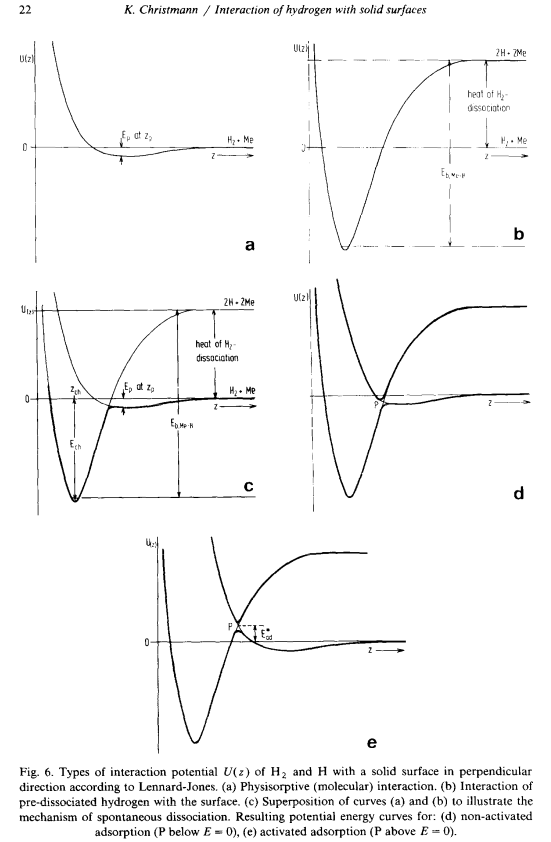
\includegraphics{Christmann_fig06.png}
\caption{Christmann\_fig06.png}
\end{figure}

    As was pointed out before, there will be only small attractive
interaction forces of van der Waals origin as the \(H_2\) molecule is
sufficiently close to the surface giving rise to a shallow interaction
potential (depth \(E_{phys}\)) at a distance \(z_{phys}\) from the
surface.

Как уже отмечалось, при достаточно близком расположении молекулы \(H_2\)
к поверхности будут существовать лишь небольшие силы притяжения
ван-дер-ваальсова происхождения, что приводит к появлению малого
потенциала взаимодействия (глубина \(E_{phys}\)) на расстоянии
\(z_{phys}\) от поверхности.

At present, there are not too many experimental verifications of this
co-called ``physisorptive'' interaction, but a variety of theoretical
predictions of this process {[}80-82{]}. The respective binding energies
of the H\_2 molecule to the surface (here, any solid surface can be
visualized) are very small; they range between 3.5 and 15 kJ/mol, depend
ing on the system. For the experiment this means that the respective
investiga tions have to be carried out at liquid helium temperatures.
Reports on the physisorption of \(H_2\) on graphite {[}83,84{]} or on
copper {[}85,86{]} and silver {[}87{]} are mentioned in this context;
also, the interaction potential depths for \(HD\) (\(D_2\)) on Au(111)
have been determined recently by molecular beam scattering experiments
{[}37{]}. This method is most commonly employed for the determina tion
of \(H_2\)-alkali halide interaction potentials, e.g., for the system
\(NaCl/H_2\) {[}88{]}.

В настоящее время существует не так много экспериментальных
подтверждений этого так называемого «физикорптивного» взаимодействия, но
зато множество теоретических предсказаний этого процесса {[}80-82{]}.
Соответствующие энергии связывания молекулы H\_2 с поверхностью (здесь
можно представить любую твердую поверхность) очень малы; они колеблются
между 3,5 и 15 кДж/моль, в зависимости от системы. Для эксперимента это
означает, что соответствующие исследования должны проводиться при
температуре жидкого гелия. В этом контексте можно упомянуть сообщения о
физорбции \(H_2\) на графите {[}83,84{]} или на меди {[}85,86{]} и
серебре {[}87{]}; кроме того, недавно были определены глубины потенциала
взаимодействия для \(HD\) (\(D_2\)) на Au(111) с помощью экспериментов
по молекулярно-пучковому рассеянию {[}37{]}. Наиболее часто этот метод
используется для определения потенциалов взаимодействия \(H_2\)-щелочных
галогенидов, например, для системы \(NaCl/H_2\) {[}88{]}.

Quite frequently the question comes up as to the possibility of
molecular hydrogen (\(H_2\)) adsorption at temperatures well above 20 K
(which is regarded as the highest possible temperature at which true
physisorption of hydrogen can occur). Reports in the past in which it
was claimed that molecular hydrogen had been detected between 100 and
300 K mostly turned out to suffer from \(H_2 O\) impurities, thermal
gradients and spurious desorption in temperature programmed thermal
desorption spectroscopy.

Довольно часто возникает вопрос о возможности адсорбции молекулярного
водорода (\(H_2\)) при температурах значительно выше 20 К (которая
считается максимально возможной температурой, при которой может
происходить истинная физическая адсорбция водорода). Сообщения прошлого,
в которых утверждалось, что молекулярный водород был обнаружен в
диапазоне от 100 до 300 К, в основном оказывались следствием примесей
\(H_2 O\), тепловых градиентов и ложной десорбции в спектроскопии
термопрограммированной термической десорбции.

However, there was a report quite recently by Martensson et al. {[}89{]}
in which molecular \(H_2\) adsorption was found on edge sites of a
stepped Ni(lOO) (Ni(510)) surface by means of vibrational loss (EELS)
spectroscopy, at a temperature around 100 K. A broad weak vibrational
band (vu-n) appeared after saturation of the atomic H states, between
350 and 450 meV. It is stated that this molecular adsorption can only
occur after the chemisorption channel (see section 2.5) is blocked by a
saturated adsorbed layer. An electronic model is proposed to reconcile
both the molecular ``chemisorption'' and the location of the adsorption
site at the edges of the terraces.

Однако совсем недавно Мартенссон и др. {[}89{]} сообщили, что с помощью
спектроскопии колебательных потерь (EELS) при температуре около 100 К на
краевых участках ступенчатой поверхности Ni(lOO) (Ni(510)) была
обнаружена адсорбция молекулярного \(H_2\). Широкая слабая колебательная
полоса (vu-n) появилась после насыщения атомных состояний H, между 350 и
450 мэВ. Утверждается, что такая молекулярная адсорбция может
происходить только после того, как канал хемосорбции (см. раздел 2.5)
блокируется насыщенным адсорбированным слоем. Предложена электронная
модель, позволяющая согласовать как молекулярную «хемосорбцию», так и
расположение адсорбционного участка на краях террас.

\section{2.5. Chemisorption}\label{chemisorption}

A completely different interaction pattern is observed, if the \(H_2\)
molecule is dissociated into the atoms prior to the interaction. Since
the dissociation energy has to be spent on the system first, the
potential energy curve in fig. 6b starts 435 kJ above the energy zero
level on the right-hand side of the diagram. Now, the 1s wave functions
of the H atoms tend to form chemical bonds with the surface material
which in many cases will lead to the situation depicted in fig. 6b:
Strong attractive interaction forces lead to a pronounced lowering of
the potential energy of the system as the H atoms are brought close to
the surface. The depths of the potential wells range between 500 and 600
kJ/mol and simply represent the energy content of a single H-surface
atom bond. Note that this quantity is gained twice since one H, molecule
dissociates into two atoms.

\section{2.5.
Хемосорбция}\label{ux445ux435ux43cux43eux441ux43eux440ux431ux446ux438ux44f}

Совершенно иная картина взаимодействия наблюдается, если молекула
\(H_2\) диссоциирует на атомы до начала взаимодействия. Поскольку
энергия диссоциации сначала должна быть потрачена на систему, кривая
потенциальной энергии на рис. 6b начинается на 435 кДж выше нулевого
уровня энергии в правой части диаграммы. Теперь волновые функции 1s
атомов H стремятся образовать химические связи с материалом поверхности,
что во многих случаях приводит к ситуации, изображенной на рис. 6b:
Сильные силы притяжения приводят к выраженному понижению потенциальной
энергии системы по мере приближения атомов H к поверхности. Глубина
потенциальных ям лежит в диапазоне 500-600 кДж/моль и просто
представляет собой энергетическое содержание одной связи атома H с
поверхностью. Обратите внимание, что эта величина получается дважды,
поскольку одна молекула H диссоциирует на два атома.

Again, experiments are scarce in which this interaction energy is
determined directly - the problem is that a beam of H atoms has to be
prepared which either requires a very hot tungsten filament {[}90{]} or
a high frequency ischarge {[}91{]} in order to supply the \(H_2\) gas
atmosphere with sufficient energy. Recent experiments in which silicon
surfaces were subjected to interaction with a H atom beam showed a
strong and rapid chemical attack of the H atoms to form silicon hydride
(silane) compounds {[}92,93{]}. Although there are no experiments known
at present it is believed that the interaction of H atoms with, e.g.,
alkali or alkaline earth metals will immediately lead to the formation
of the respective hydrides, whereby these processes are highly
exothermic. On Ni(110) single crystal surfaces the interaction with a H
atom beam has been reported to reveal the existence of excited
interaction com plexes, the so-called ``hot-precursor states'' {[}94{]}
which have also been treated theoretically.

Экспериментов, в которых эта энергия взаимодействия определялась бы
напрямую, опять же мало - проблема в том, что необходимо подготовить
пучок атомов H, для чего требуется либо очень горячая вольфрамовая нить
{[}90{]}, либо высокочастотный разряд {[}91{]}, чтобы обеспечить газовую
атмосферу \(H_2\) достаточной энергией. Недавние эксперименты, в которых
поверхности кремния подвергались взаимодействию с пучком атомов H,
показали сильную и быструю химическую атаку атомов H с образованием
соединений гидрида кремния (силанов) {[}92,93{]}. Хотя в настоящее время
эксперименты не известны, считается, что взаимодействие атомов Н,
например, со щелочными или щелочноземельными металлами немедленно
приведет к образованию соответствующих гидридов, причем эти процессы
являются сильно экзотермическими. На поверхности монокристаллов Ni(110)
при взаимодействии с пучком атомов H было обнаружено существование
возбужденных комплексов взаимодействия, так называемых «горячих
прекурсорных состояний» {[}94{]}, которые также были теоретически
обработаны.

    \begin{tcolorbox}[breakable, size=fbox, boxrule=1pt, pad at break*=1mm,colback=cellbackground, colframe=cellborder]
\prompt{In}{incolor}{ }{\boxspacing}
\begin{Verbatim}[commandchars=\\\{\}]

\end{Verbatim}
\end{tcolorbox}

    \section{2.9. Surface diffusion}\label{surface-diffusion}

    Comparatively much less experimental and theoretical effort has been
devoted to the surface diffusion of hydrogen. In the single particle
picture we understand the surface diffusion as a process in which a
given H atom adsorbed on a site ``A'' can reach a site ``B'' (of
identical symmetry) of the surface lattice. More complicated are
migration processes which comprise the correlated diffusion of two or
several adjacent adsorbed H atoms. Of course, the diffusion of a single
particle will also strongly depend on the surface coverage, i.e., depend
on the number of ``empty'' adsorption sites through which ``hopping''
and diffusion steps can occur.

Although quite often neglected in adsorption studies surface diffusion
is a very important processes. It influences especially the kinetics of
the adsorption and desorption reaction.

When dealing with surface diffusion one must distinguish lateral
mobility in the physisorbed (i.e., molecular) and in the chemisorbed
state.

    \section{2.9. Поверхностная
диффузия}\label{ux43fux43eux432ux435ux440ux445ux43dux43eux441ux442ux43dux430ux44f-ux434ux438ux444ux444ux443ux437ux438ux44f}

    Сравнительно меньше экспериментальных и теоретических усилий было
посвящено поверхностной диффузии водорода. В одночастичной картине мы
понимаем поверхностную диффузию как процесс, в котором данный атом H,
адсорбированный на участке «A», может достичь участка «B» (идентичной
симметрии) поверхностной решетки. Более сложными являются миграционные
процессы, включающие в себя коррелированную диффузию двух или нескольких
соседних адсорбированных атомов H. Разумеется, диффузия отдельной
частицы также будет сильно зависеть от покрытия поверхности, то есть от
количества «пустых» адсорбционных участков, через которые могут
происходить «прыжки» и диффузионные шаги.

Хотя в исследованиях адсорбции поверхностной диффузией часто
пренебрегают, она является очень важным процессом. Она особенно сильно
влияет на кинетику реакции адсорбции и десорбции.

При рассмотрении поверхностной диффузии необходимо различать латеральную
подвижность в физисорбированном (т.е. молекулярном) и в
хемосорбированном состоянии.

    \begin{tcolorbox}[breakable, size=fbox, boxrule=1pt, pad at break*=1mm,colback=cellbackground, colframe=cellborder]
\prompt{In}{incolor}{ }{\boxspacing}
\begin{Verbatim}[commandchars=\\\{\}]

\end{Verbatim}
\end{tcolorbox}

    The corrugation of any periodic surface is certainly much less
pronounced in the van der Waals potential minimum several angstroms away
from the surface, with the consequence that the mobility in this weakly
held state is usually very high. If this physisorbed state is
significantly populated by \(H_2\) molecules we commonly observe the
typical ``precursor'' state kinetics of adsorption (cf. section 3.4)
which involves a trapped but still mobile \(H_2\) molecule travelling
over large distances (many lattice constants) parallel to the surface in
search of an unoccupied dissociation site.

Волнистость любой периодической поверхности, конечно, гораздо менее
выражена в минимуме ван-дер-ваальсова потенциала в нескольких ангстремах
от поверхности, вследствие чего подвижность в этом слабоудерживаемом
состоянии обычно очень высока. Если это физико-сорбированное состояние
значительно заселено молекулами \(H_2\), мы обычно наблюдаем типичную
кинетику адсорбции в состоянии «предшественника» (см. раздел 3.4),
которая включает в себя захваченную, но все еще подвижную молекулу
\(H_2\) перемещающейся на большие расстояния (много констант решетки)
параллельно поверхности в поисках незанятого места диссоциации.

    A different situation is faced once a H, molecule has been dissociated
into the H atoms which then are located in the substantially deeper
chemisorption potential wells. As fig. 20 illustrates there is a lateral
variation of the chemisorption energy by \(\approx 1/10\) of the heat of
adsorption (as experience shows) whereby a sinusoidal potential energy
variation in \(x-y\) direction can be assumed. In other words, the
\(E(z)\) chemisorption potential is modulated in \(x-y\) direction
according to the periodicity of the surface lattice. In order for an
adsorbed \(H\) atom to get from one minimum to an adjacent one a certain
amount of energy is required, namely, the activation energy for
diffusion, \(E^{*}_{diff}\), unless tunnelling is possible. In analogy
with the Frenkel equation we may define a residence time
\(\tau^{\prime}\) of a H atom in a given adsorption site as

\(\tau^{\prime} = \tau^{\prime}_{0} \, exp \left(\frac{E^{*}_{diff}}{kT} \right)\).(14)

In the multi-particle description and by introducing \(D\) this
expression may be transformed to

\(D(T) = D_{0} \, exp \left(-\frac{E^{*}_{diff}}{kT} \right)\).(15)

in which D(T) is defined by Fick's law in terms of the time dependence
concentration divided by the spatial variation of the concentration
dimension, \(x\) (number of particles per \(cm^2\))

\(D = - \left(\frac{\partial N}{\partial t}\right)_x \Big/ \left(\frac{\partial N}{\partial x}\right)_t\).

    \begin{tcolorbox}[breakable, size=fbox, boxrule=1pt, pad at break*=1mm,colback=cellbackground, colframe=cellborder]
\prompt{In}{incolor}{ }{\boxspacing}
\begin{Verbatim}[commandchars=\\\{\}]

\end{Verbatim}
\end{tcolorbox}

    \section{3. The multi-particle interaction and collective
phenomena}\label{the-multi-particle-interaction-and-collective-phenomena}

    We may directly continue the considerations of the foregoing section as
we discuss the behavior of a whole ensemble of adsorbed hydrogen
molecules or atoms on a periodic surface. Two major points have to be
kept in mind:

\begin{enumerate}
\def\labelenumi{(\roman{enumi})}
\item
  The surface exhibits a lateral periodic potential, i.e., provides sort
  of checkerboard of adsorption sites. Only for the zero coverage limit
  all these sites can be assumed to be identical (fig. 20a).
\item
  Even two equally adsorbed particles may interact with each other
  whereby the strength of interaction depends on their mutual distance.
  This leads to a superposition of the sinusoidal potential \(E(x, y)\)
  and the mutual interaction potential \(E_{H-H}\) (which may be
  attractive or repulsive). These two situations are depicted in figs.
  20b and 20c. It will be shown in the following section that it is this
  modification of the energetic structure of a surface that largely
  governs the thermodynamics but also influences the kinetics of
  adsorption.
\end{enumerate}

    \section{3. Многочастичное взаимодействие и коллективные
явления}\label{ux43cux43dux43eux433ux43eux447ux430ux441ux442ux438ux447ux43dux43eux435-ux432ux437ux430ux438ux43cux43eux434ux435ux439ux441ux442ux432ux438ux435-ux438-ux43aux43eux43bux43bux435ux43aux442ux438ux432ux43dux44bux435-ux44fux432ux43bux435ux43dux438ux44f}

    Мы можем непосредственно продолжить рассуждения предыдущего раздела,
обсуждая поведение целого ансамбля адсорбированных молекул или атомов
водорода на периодической поверхности. При этом следует иметь в виду два
основных момента:

\begin{enumerate}
\def\labelenumi{(\roman{enumi})}
\item
  Поверхность имеет латеральный периодический потенциал, т.е.
  представляет собой своего рода шахматную доску адсорбционных площадок.
  Только в пределе нулевого покрытия можно считать, что все эти участки
  идентичны (рис. 20a).
\item
  Даже две одинаково адсорбированные частицы могут взаимодействовать
  друг с другом, причем сила взаимодействия зависит от их взаимного
  расстояния. Это приводит к суперпозиции синусоидального потенциала
  \(E(x, y)\) и потенциала взаимного взаимодействия \(E_{H-H}\) (который
  может быть притягивающим или отталкивающим). Эти две ситуации
  изображены на рис. 20b и 20c. В следующем разделе будет показано, что
  именно эта модификация энергетической структуры поверхности в
  значительной степени регулирует термодинамику, но также влияет на
  кинетику адсорбции.
\end{enumerate}

    \begin{figure}
\centering
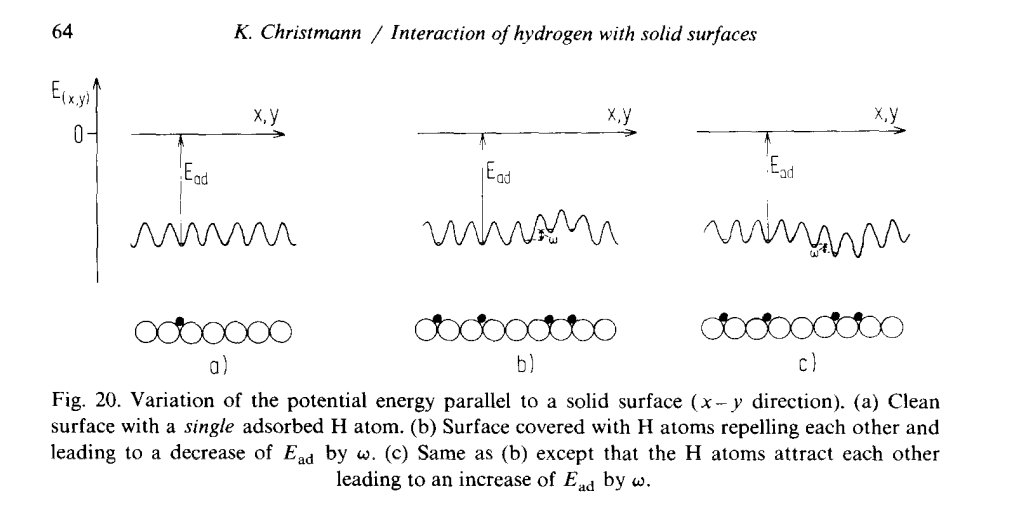
\includegraphics{Christmann_fig20.png}
\caption{Christmann\_fig20.png}
\end{figure}

    \section{3.2. The coverage dependence of the heat of
adsorption}\label{the-coverage-dependence-of-the-heat-of-adsorption}

    On the experimental side one of the most interesting questions is
concerned with the magnitude and with the sign of the lateral
interaction forces, i.e., whether they are attractive or repulsive. We
shall henceforth use the symbol \(\omega_{lj}\) for the interaction
energy between the atom \(i\) and its neighbor \(j\), and we define
\(\omega > 0\) as an attractive and \(\omega < 0\) as a repulsive
energy.

It has been known for a long time that with most of the adsorption
systems the highest energies of adsorption are obtained at small
adsorbate coverages, and a more or less pronounced decay of the heat of
adsorption follows as the concentration of the adsorbate increases.
Clearly, this kind of behavior would suggest the operation of repulsive
mutual interactions between the adatoms. In a very simple case, namely
the dipole-dipole interaction between positively charged adsorbed alkali
atoms, these interactions can be calculated fairly accurately, and a
good agreement with experimental data is obtained.

However, if we deal with almost neutral adatoms held by a covalent bond
any predictions are much more difficult. In addition to the most
commonly observed repulsive forces in some cases also attractive
interactions may dominate, at least in a certain coverage range. This
then leads to an increase in the heat of adsorption with island
formation and condensation phenomena.

Apparently, we can obtain the relevant information as to which
interaction forces dominate from a measurement of the coverage
(concentration) dependence of the heat of adsorption.

This in turn can be achieved either by isosteric heat measurements
(which require the mapping of adsorption isotherms therms
(\(\Theta(P)_T\)) or isobars (\(\Theta(T)_P\))), or by performing
thermal desorption experiments with varying initial coverage. Most
important is the isosteric heat of adsorption, \(q_{st}\), which is
defined thermodynamically as the latent heat exchanged in the phase
equilibrium: gas phase (pressure \(P\)) - adsorbed phase according to

\(q_{st} = R T^2 \left( \frac{\partial \, \left(ln P\right)}{\partial T}\right)_{\Theta}\).
(17)

Sometimes it is necessary to distinguish of adsorption which are related
by

\(q_{diff} = \left( \frac{\partial \, q_{int}}{\partial n_A}\right)_{T}\)
(18)

and in which expression \(n_A\) denotes the number of moles of adsorbed
gas of kind \(A\). \(q_st\) and \$q\_\{diff\} are interrelated by

\(q_{st} = q_{diff} + R T\), (19)

the difference at 300 \(K\) being of the order of 2.5 \(kJ/mol\).

    \section{3.2. Зависимость теплоты адсорбции от
покрытия}\label{ux437ux430ux432ux438ux441ux438ux43cux43eux441ux442ux44c-ux442ux435ux43fux43bux43eux442ux44b-ux430ux434ux441ux43eux440ux431ux446ux438ux438-ux43eux442-ux43fux43eux43aux440ux44bux442ux438ux44f}

С экспериментальной стороны один из наиболее интересных вопросов
касается величины и знака сил латерального взаимодействия, т.е. являются
ли они притягивающими или отталкивающими. В дальнейшем мы будем
использовать символ \(\omega_{lj}\) для обозначения энергии
взаимодействия между атомом \(i\) и его соседом \(j\), и мы определяем
\(\omega > 0\) как притягивающую, а \(\omega < 0\) как отталкивающую
энергию.

Давно известно, что в большинстве адсорбционных систем наибольшие
энергии адсорбции достигаются при малых покрытиях адсорбата, а с
увеличением концентрации адсорбата следует более или менее выраженный
спад теплоты адсорбции. Очевидно, что такое поведение свидетельствует о
наличии отталкивающих взаимодействий между адатомами. В очень простом
случае, а именно в случае диполь-дипольного взаимодействия между
положительно заряженными адсорбированными атомами щелочи, эти
взаимодействия могут быть рассчитаны достаточно точно, и получено
хорошее согласие с экспериментальными данными.

Однако если мы имеем дело с почти нейтральными адатомами, удерживаемыми
ковалентной связью, любые предсказания оказываются гораздо более
сложными. Помимо наиболее часто наблюдаемых отталкивательных сил в
некоторых случаях могут преобладать и притягивающие взаимодействия, по
крайней мере, в определенном диапазоне охвата. Это приводит к увеличению
теплоты адсорбции с образованием островков и явлениями конденсации.

По-видимому, соответствующую информацию о том, какие силы взаимодействия
доминируют, можно получить из измерения зависимости теплоты адсорбции от
охвата (концентрации).

Это, в свою очередь, может быть достигнуто либо путем изостерических
измерений теплоты (которые требуют отображения изотерм адсорбции
(\(\Theta(P)_T\)) или изобар (\(\Theta(T)_P\))), либо путем проведения
термических экспериментов по десорбции с изменяющимся начальным
покрытием. Наиболее важной является изостерическая теплота адсорбции,
\(q_{st}\), которая термодинамически определяется как скрытая теплота,
обмениваемая в фазовом равновесии: газовая фаза (давление \(P\)) -
адсорбированная фаза в соответствии с формулой

\(q_{st} = R T^2 \left( \frac{\partial \, \left(ln P\right)}{\partial T}\right)_{\Theta}\).
(17)

Иногда необходимо различать адсорбции, которые связаны между собой
следующим образом

\(q_{diff} = \left( \frac{\partial \, q_{int}}{\partial n_A}\right)_{T}\)
(18)

и в котором выражение \(n_A\) обозначает количество молей
адсорбированного газа вида \(A\). \(q_st\) и \$q\_\{diff\} связаны между
собой следующим образом

\(q_{st} = q_{diff} + R T\), (19)

разница при 300 \(K\) составляет порядка 2,5 \(kJ/mol\).

    \begin{figure}
\centering
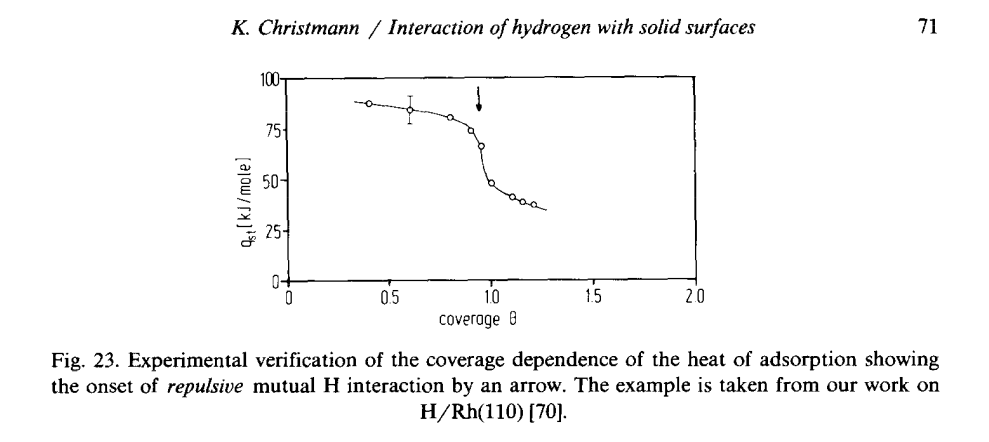
\includegraphics{Christmann_fig23.png}
\caption{Christmann\_fig23.png}
\end{figure}

    \begin{figure}
\centering
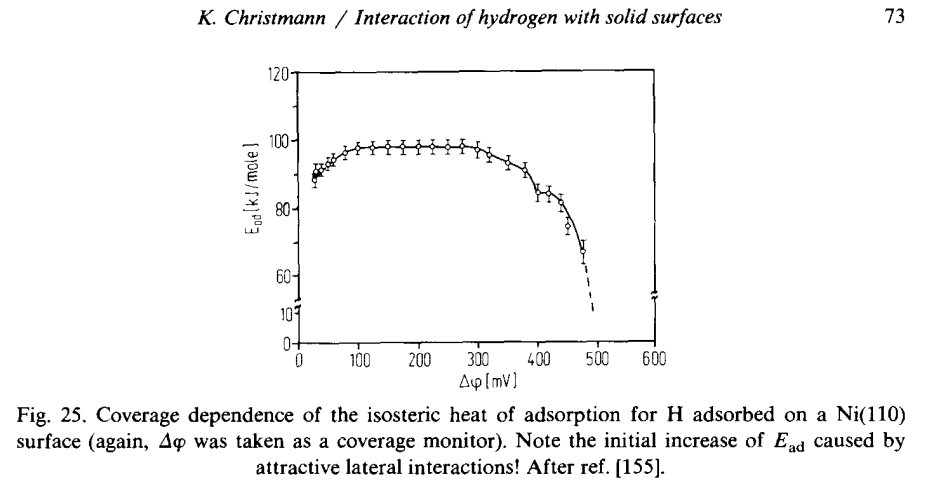
\includegraphics{Christmann_fig25.png}
\caption{Christmann\_fig25.png}
\end{figure}

    \begin{figure}
\centering
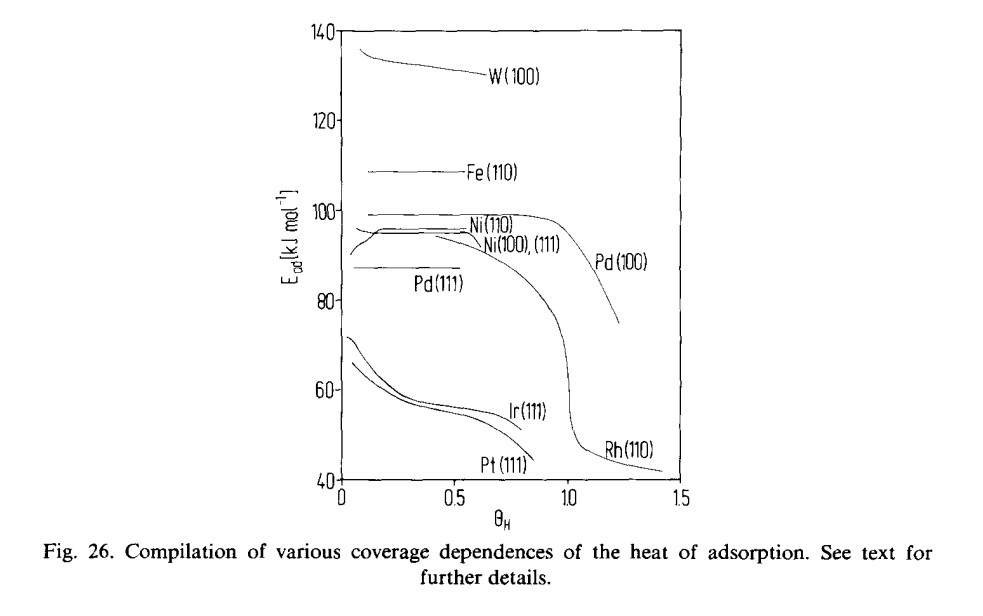
\includegraphics{Christmann_fig26.png}
\caption{Christmann\_fig26.png}
\end{figure}

    \section{3.4. The coverage dependence of the H adsorption
kinetics}\label{the-coverage-dependence-of-the-h-adsorption-kinetics}

    In section 2.3 we have discussed probable mechanisms leading to hydrogen
adsorption, and have introduced the initial sticking probability,
\(s_0\), as the crucial parameter that governs the initial rate of
adsorption.

However, any time a \(H_2\) molecule dissociates and chemisorbs it
finally occupies two adsorption sites. The simplest model to describe
this situation has been given by Langmuir {[}240{]} which is
characterized by the following assumptions: At all coverages sites with
identical symmetry are occupied, which also implies that the surface is
homogeneous.

There are no lateral interactions between the adatoms, and the particles
are considered immobile after having collided with the surface.

For completely mobile adsorption (mobile in the chemisorbed state) a
simple second order rate expression can be derived with:

\(dn_{ad} / dt = s_0 f\left(\Theta\right) P_{H_2} \left(2 \pi m k T\right)^{-1/2}\)
(21)

(Hertz-Knudsen equation), with

\(f\left(\Theta\right) = \left(1 - \Theta\right)^2\). (22)

(If the layer is immobile, e.g., at very low temperatures,
\(f\left(\Theta\right)\) must be modified to yield (with z the number of
nearest neighbor sites)):

\(f\left(\Theta\right) = z \left(1 - \Theta\right)^2 \left(z - \Theta\right)^{-1}\).
(23).

    \section{3.4. Зависимость кинетики адсорбции H от
покрытия}\label{ux437ux430ux432ux438ux441ux438ux43cux43eux441ux442ux44c-ux43aux438ux43dux435ux442ux438ux43aux438-ux430ux434ux441ux43eux440ux431ux446ux438ux438-h-ux43eux442-ux43fux43eux43aux440ux44bux442ux438ux44f}

    В разделе 2.3 мы обсудили возможные механизмы, приводящие к адсорбции
водорода, и ввели начальную вероятность прилипания, \(s_0\), как
важнейший параметр, определяющий начальную скорость адсорбции.

Однако каждый раз, когда молекула \(H_2\) диссоциирует и
хемосорбируется, она в конечном итоге занимает два адсорбционных
участка. Простейшая модель для описания этой ситуации была предложена
Ленгмюром {[}240{]}, которая характеризуется следующими предположениями:
На всех покрытиях заняты сайты с одинаковой симметрией, из чего также
следует, что поверхность однородна.

Латеральные взаимодействия между адатомами отсутствуют, и частицы
считаются неподвижными после столкновения с поверхностью.

Для полностью подвижной адсорбции (подвижной в хемосорбированном
состоянии) может быть получено простое выражение скорости второго
порядка:

\(dn_{ad} / dt = s_0 f\left(\Theta\right) P_{H_2} \left(2 \pi m k T\right)^{-1/2}\)
(21)

(уравнение Герца-Кнудсена), причем

\(f\left(\Theta\right) = \left(1 - \Theta\right)^2\). (22)

(Если слой неподвижен, например, при очень низких температурах,
\(f\left(\Theta\right)\) должно быть изменено, чтобы получить (при z -
число ближайших соседей):

\(f\left(\Theta\right) = z \left(1 - \Theta\right)^2 \left(z - \Theta\right)^{-1}\).
(23).

    \begin{tcolorbox}[breakable, size=fbox, boxrule=1pt, pad at break*=1mm,colback=cellbackground, colframe=cellborder]
\prompt{In}{incolor}{ }{\boxspacing}
\begin{Verbatim}[commandchars=\\\{\}]

\end{Verbatim}
\end{tcolorbox}

    There have been numerous experimental and theoretical articles published
which focus on the determination and description of the sticking
probability-coverage function \(s(\Theta)\). An excellent review here is
provided by the work of Morris et al. {[}78{]}.

The rate of adsorption can principally be obtained from the variation of
any physical quantity with time which is directly related to the adatom
concentration.

The H-induced work function, \(\Delta \varphi\), has already been
mentioned; other quantities are, e.g., the optical absorption
coefficient, the surface conductivity or the thermopower {[}241{]}.
Another straightforward way to determine the coverage is direct
gravimetry.

We refer to the work by Kasemo and Tornqvist {[}242{]} who followed the
amount of hydrogen adsorbed on \(Pt(111)\) by weighing even fractions of
a H monolayer by means of a quartz microbalance.

The peak intensities of Auger transitions or X-ray photoelectron spectra
are quite suitable to monitor the surface coverage of heavier adsorbates
such as \(N_2\), \(CO\) or \(O_2\). For physical reasons this fails in
the case of \(H\) adsorption.

    Опубликовано множество экспериментальных и теоретических статей,
посвященных определению и описанию функции вероятности налипания
\(s(\Theta)\). Отличный обзор здесь представлен в работа Морриса и
других {[}78{]}.

Скорость адсорбции может быть в основном получена из изменения любой
физической величины со временем, которая непосредственно связана с
концентрацией адатомов.

Уже упоминалась индуцированная Н-функция, \(\Delta \varphi\); другими
величинами могут быть, например, коэффициент оптического поглощения,
поверхностная проводимость или тепловая мощность {[}241{]}. Другим
простым способом определения покрытия является прямая гравиметрия.

Мы ссылаемся на работу Касемо и Торнквиста {[}242{]}, которые следили за
количеством водорода, адсорбированного на \(Pt(111)\) путем взвешивания
равномерных долей монослоя \(H\) с помощью кварцевых микровесов.

Интенсивности пиков оже-переходов или рентгеновских фотоэлектронных
спектров вполне подходят для мониторинга покрытия поверхности более
тяжелыми адсорбатами, такими как \(N_2\), \(CO\) или \(O_2\). По
физическим причинам это не удается в случае адсорбции \(H\) адсорбции.

    \begin{tcolorbox}[breakable, size=fbox, boxrule=1pt, pad at break*=1mm,colback=cellbackground, colframe=cellborder]
\prompt{In}{incolor}{ }{\boxspacing}
\begin{Verbatim}[commandchars=\\\{\}]

\end{Verbatim}
\end{tcolorbox}

    Probably most commonly used, however, is the thermal desorption
technique.

Here, the adsorption is interrupted at time \(t_0\), and the sample is
heated such that all adsorbed adatoms leave the surface by thermal
desorption.

In a closed system, the resulting partial pressure increase,
\(\Delta P\), can be measured, and with the gas temperature, \(T_g\),
and the system volume, \(V\), being known, the average rate of
adsorption up to time \(t\) is given by

\(\left<\frac{d n_{ad}}{d t}\right> = \frac{1}{t}\left(\frac{V \Delta P}{k T_g}\right)\)

where \(k\) is Boltzmann's constant.

In common TPD spectroscopy the system is pumped and one rather obtains a
transient pressure increase upon desorption. Likewise, the number of
particles adsorbed at time \(t\), \(N_t\), is obtained by a numerical
integration of the TPD curve. In this case, the sample area \(A\) and
the effective pumping speed, \(S_{eff} = V/\tau\), must be known (T is a
time constant):

\(N_t = \frac{S_{eff}}{A k T_g} \int R(t) \,\, dt. \,\,\,(25)\)

There are numerous examples in the literature where coverages and
adsorption kinetics have been determined in this way {[}1,155,158{]}.

    Однако, вероятно, наиболее часто используется метод термической
десорбции.

В этом случае адсорбция прерывается в момент времени \(t_0\), и образец
нагревается так, что все адсорбированные адатомы покидают поверхность
путем термической десорбции.

В закрытой системе можно измерить результирующее увеличение парциального
давления, \(\Delta P\), и при известной температуре газа, \(T_g\), и
объеме системы, \(V\), средняя скорость адсорбции до времени \(t\)
определяется следующим образом

\(\left<\frac{d n_{ad}}{d t}\right> = \frac{1}{t}\left(\frac{V \Delta P}{k T_g}\right)\)

где \(k\) - постоянная Больцмана.

В обычной TPD-спектроскопии система накачивается насосом, и при
десорбции скорее наблюдается переходное повышение давления. Аналогично,
число частиц, адсорбированных в момент времени \(t\), \(N_t\),
получается путем численного интегрирования кривой TPD. В этом случае
необходимо знать площадь образца \(A\) и эффективную скорость откачки,
\(S_{eff} = V/\tau\) (T - постоянная времени):

\(N_t = \frac{S_{eff}}{A k T_g} \int R(t) \,\, dt. \,\,\,(25)\)

В литературе имеется множество примеров, когда покрытия и кинетика
адсорбции были определены таким образом {[}1,155,158{]}.

    Experience shows that there is hardly an example that there is hardly an
example for a clear Langmuir adsorption kinetics. A second-order
adsorption was reported for H on \(Rh(111)\) by Yates et al. {[}243{]}
and for \(H\) on \(Ir(111)\) by Engstrom et al. {[}244{]}. Several other
more previous reports have either not been performed on single crystal
surfaces or under not very well defined experimental conditions and have
to be viewed at with some care.

Relatively often, however, the hydrogen adsorption seems to obey a
first-order rate expression, i.e.,

\(f\left(\Theta\right) = 1 - \Theta\). (26)

which is expected for molecular (associative) adsorption only. Examples
here are the systems H on \(Ni(111)\) at 300 K {[}155{]}, H on
\(Ir(110)-1 \times 2\) (the \(\beta_2\) state) {[}245{]}, \(H\) on
\(Pt(110)-1 \times 2\) {[}244{]}, or H on \(Ru(0001)\) (the negatively
``N'' polarized state) {[}113{]}.

In none of these cases, however, was there any indication for a
molecular H, adsorption. A possible explanation for the first order
behavior would be that the adsorption proceeds via an island growth
mechanism so that the uncovered surface area would be proportional to
\(1 - \Theta\).

Another possibility could be that the dissociation is not
rate-determining, but rather the trapping of the molecule. This was,
e.g., proposed for H adsorption on Ru(0001) into the ``N'' sites by
Feulner and Menzel {[}113{]}.

    Опыт показывает, что вряд ли можно найти пример четкой ленгмюровской
кинетики адсорбции. Адсорбция второго порядка была зарегистрирована для
H на \(Rh(111)\) Йейтсом и др {[}243{]} и для \(H\) на \(Ir(111)\)
Энгстромом и др {[}244{]}. Некоторые другие более ранние сообщения либо
не были выполнены на монокристаллических поверхностях, либо при не очень
хорошо определенных экспериментальных условиях, и к ним следует
относиться с некоторой осторожностью.

Относительно часто, однако, адсорбция водорода подчиняется выражению
скорости первого порядка, т.е,

\(f\left(\Theta\right) = 1 - \Theta\). (26)

что ожидается только для молекулярной (ассоциативной) адсорбции.
Примерами здесь являются системы H на \(Ni(111)\) при 300 K {[}155{]}, H
на \(Ir(110)-1 \times 2\) (состояние \(\beta_2\)) {[}245{]}, \(H\) на
\(Pt(110)-1 \times 2\) {[}244{]}, или H на \(Ru(0001)\) (отрицательно
«N» поляризованное состояние) {[}113{]}.

Однако ни в одном из этих случаев не было никаких признаков молекулярной
адсорбции H. Возможным объяснением поведения первого порядка может быть
то, что адсорбция происходит по механизму роста островков, так что
площадь непокрытой поверхности пропорциональна \(1 - \Theta\).

Другая возможность заключается в том, что диссоциация не является
определяющей скоростью, а скорее является ловушкой для молекулы. Это
было предложено, например, для адсорбции H на Ru(0001) в «N»-сайтах
Фойльнером и Менцелем {[}113{]}.

    \begin{tcolorbox}[breakable, size=fbox, boxrule=1pt, pad at break*=1mm,colback=cellbackground, colframe=cellborder]
\prompt{In}{incolor}{ }{\boxspacing}
\begin{Verbatim}[commandchars=\\\{\}]

\end{Verbatim}
\end{tcolorbox}

    So it appears that deviations from the simple Langmuir type of
adsorption are the rule, for a number of reasons. Again, the influence
of adatom-adatom interactions can be very pronounced.

One immediately realizes that, e.g., island formation caused by
attractive interaction forces creates two surface areas with different
particle densities in which the sticking could be different, and
deviations from eq. (22) occur.

Kinetic models can be set up to describe the rate of adsorption in terms
of the lateral interaction forces. Here, the quasi-chemical
approximation is often used {[}246{]}.

However, an attempt to quantitatively model the adsorption kinetics
merely on the basis of lateral interactions frequently fails, because
the existence of weakly held trapping states, the so-called precursor
states, modifies the adsorption kinetics considerably. The reason is
that the trapped particles are usually very mobile; they diffuse across
the surface and can very effectively search for an empty adsorption
site. In this case, one observes the typical convex \(s(\Theta)\)
dependence in which \(s\) does almost not drop until medium coverages
but sharply falls as the population of the adsorption sites has
proceeded such that the molecule can no longer find an empty site while
diffusing across the surface in the precursor.

    Таким образом, получается, что отклонения от простого ленгмюровского
типа адсорбции являются правилом по ряду причин. Опять же, влияние
адатом-адатомных взаимодействий может быть очень выраженным.

Сразу становится понятно, что, например, образование островков,
вызванное силами притяжения, создает две поверхности области с разной
плотностью частиц, в которых прилипание может быть разным, и возникают
отклонения от уравнения (22).

Для описания скорости адсорбции в терминах сил латерального
взаимодействия могут быть созданы кинетические модели. Здесь часто
используется квазихимическое приближение {[}246{]}.

Однако попытка количественного моделирования кинетики адсорбции только
на основе латеральных взаимодействий часто не удается, поскольку
существование слабоудерживаемых состояний ловушки, так называемых
состояний-предшественников, значительно изменяет кинетику адсорбции.
Причина в том, что захваченные частицы обычно очень подвижны; они
диффундируют по поверхности и могут очень эффективно искать свободный
адсорбционный участок. В этом случае наблюдается типичная выпуклая
зависимость \(s(\Theta)\), в которой \(s\) почти не падает до средних
покрытий, но резко снижается по мере заселения адсорбционных участков,
когда молекула уже не может найти свободный участок, диффундируя по
поверхности в прекурсоре.

    The influence of these precursor states on the kinetics of adsorption
was first realized by Ehrlich and by Kisliuk {[}247{]}, and later
reinvestigated by King {[}235{]}, Schbnhammer {[}237{]}, Gorte and
Schmidt {[}236{]} or Steinbrtichel {[}248{]}. Frequently analytical rate
expressions were derived which - by assuming a simple lateral
interaction energy \(\omega\) as well as probability functions for the
precursor population - could quite well predict the experimentally
observed \(s(\Theta)\) curves. An extensive consideration of this matter
can be found in the article by Morris, Bowker and King {[}78{]}.

Here we confine ourselves to the presentation of some experimental
examples that have been reported in the literature for H adsorption. A
clear evidence for the existence of a hydrogen precursor state for a
chemisorbed system was obtained for the \(Pd(100)/H\) system by Behm et
al. {[}77{]}. This is shown in fig. 28.

    Влияние этих состояний прекурсоров на кинетику адсорбции было впервые
осознано Эрлихом и Кислюком {[}247{]}, а затем вновь исследовано Кингом
{[}235{]}, Шбнхаммером {[}237{]}, Горте и Шмидтом {[}236{]} или
Штайнбртихелем {[}248{]}. Часто были получены аналитические выражения
скорости, которые - в предположении простой энергии латерального
взаимодействия \(\omega\), а также функции вероятности для популяции
прекурсоров - могли довольно хорошо предсказать экспериментально
наблюдаемые кривые \(s(\Theta)\). Подробное рассмотрение этого вопроса
можно найти в статье Морриса, Боукера и Кинга {[}78{]}.

Здесь мы ограничимся изложением некоторых экспериментальных примеров,
которые были приведены в литературе для адсорбции H. Четкое
доказательство существования состояния предшественника водорода для
хемосорбированной системы было получено для системы \(Pd(100)/H\) в
работе Behm et al {[}77{]}. Это показано на рис. 28.

    \begin{figure}
\centering
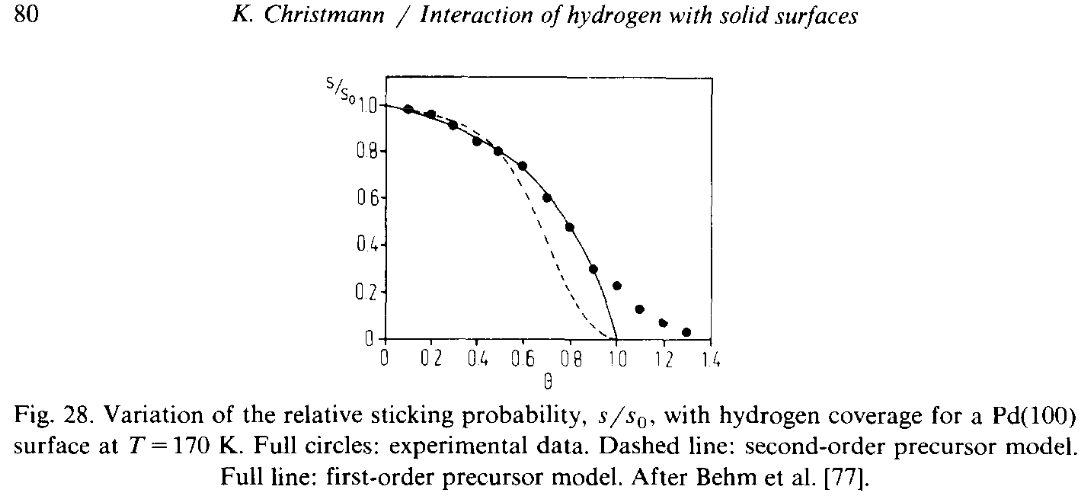
\includegraphics{Christmann_fig28.png}
\caption{Christmann\_fig28.png}
\end{figure}

    Other investigations proved the importance of these mobile precursor
states also for H on Ni(110) at temperatures below 200 K {[}249{]}, for
H on Pd(110) {[}68{]}, H on Ru(1010) {[}71{]} and Co(1010) {[}69{]}, as
well as on Rh(110) {[}70{]} and H on W(100) {[}1,250-255{]}, one of the
most frequently studied systems. In summary, it appears as if
particularly the crystallographically ``rough'' metal surface planes
would be very suited to provide a precursor state adsorption kinetics.

    Другие исследования доказали важность этих подвижных состояний
прекурсора также для H на Ni(110) при температурах ниже 200 K {[}249{]},
для H на Pd(110) {[}68{]}, H на Ru(1010) {[}71{]} и Co(1010) {[}69{]}, а
также на Rh(110) {[}70{]} и H на W(100) {[}1,250-255{]}, одной из
наиболее часто изучаемых систем. Таким образом, представляется, что
особенно кристаллографически «шероховатые» плоскости поверхности
металлов очень хорошо подходят для обеспечения кинетики адсорбции в
прекурсорном состоянии.

    Apart from the relatively distinct precursor state influence all
processes which contribute to the long-range order within the surface
region may more or less disturb the simple adsorption kinetics of eq.
(21). Among these are order-order and order-disorder phase transitions
and particularly, reconstructive phase transitions involving the
substrate surface layer. Whilst the effect of the long-range order of a
merely adsorbed H layer on \(s(\Theta)\) could not so clearly be
established experimentally the influence of a H-induced surface
reconstruction can give rise to pronounced alterations of this function
which are relatively easy to observe. An example is provided by the
H-on-Ni(110) system {[}231{]}).

    Помимо относительно четкого влияния состояния прекурсора, все процессы,
способствующие дальнему порядку в приповерхностной области, могут в
большей или меньшей степени нарушать простую кинетику адсорбции по
уравнению (21). К ним относятся фазовые переходы «порядок-беспорядок» и
«порядок-беспорядок» и, в частности, реконструктивные фазовые переходы,
затрагивающие поверхностный слой подложки. В то время как влияние
дальнего порядка просто адсорбированного слоя H на \(s(\Theta)\) не
может быть так четко установлено экспериментально, влияние
H-индуцированной реконструкции поверхности может привести к выраженным
изменениям этой функции, которые относительно легко наблюдать. В
качестве примера можно привести систему H-on-Ni(110) {[}231{]}).

    Depending on the adsorption temperature the surface under hydrogen
remains stable up to \(\Theta_H = 1.0\) and then suddenly transforms to
a \(1 \times 2\) reconstructed pairing row arrangement (this behavior is
observed for \(T_{ad} < 220 K\)) or, for \(T_{ad} > 220 K\), it
reconstructs immediately to a streaky (``Str'') (perhaps missing row)
phase.

    В зависимости от температуры адсорбции поверхность под водородом
остается стабильной до \(\Theta_H = 1.0\), а затем внезапно
трансформируется в \(1 \times 2\) реконструированное расположение парных
рядов (такое поведение наблюдается для \(T_{ad} < 220 K\)) или, для
\(T_{ad} > 220 K\), он сразу же перестраивается в полосатую («Str»)
(возможно, отсутствующую) фазу.

    Fig. 29 shows how this affects the exposure dependence of the coverage
(the slope of this curve contains the sticking coefficient \(s\)). In
fig. 29 \(\Delta \varphi\) was taken as a coverage monitor. Obviously,
the phase transformation \(1 \times 1 + 1 \times 2\) at \(\Theta = 1.0\)
gives rise to a plateau in the \(\Delta \varphi\)-exposure dependence.

    На рис. 29 показано, как это влияет на зависимость покрытия от
экспозиции (наклон этой кривой содержит коэффициент прилипания \(s\)).
На рис. 29 в качестве монитора покрытия взята \(\Delta \varphi\).
Очевидно, что фазовое превращение \(1 \times 1 + 1 \times 2\) при
\(\Theta = 1.0\) приводит к появлению плато в зависимости
\(\Delta \varphi\) от экспозиции.

    \begin{figure}
\centering
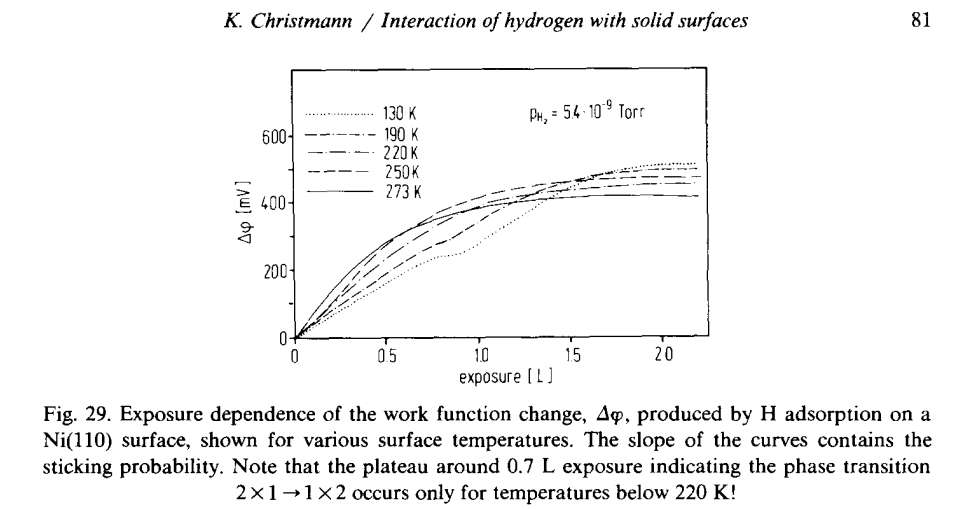
\includegraphics{Christmann_fig29.png}
\caption{Christmann\_fig29.png}
\end{figure}

    An evaluation of the true relation: coverage against exposure, however,
does not yield this plateau anymore (which apparently is only a work
function effect) but still exhibits a change of the sticking coefficient
at \(\Theta_H = 1.0\) which is more obvious from the \(s(\Theta)\) plot
of fig. 30. We deduce from this figure that the phase transformation
\(1 \times 1 \rightarrow 1 \times 2\) provides ``new'' adsorption sites
for hydrogen on which the sticking can take place more efficiently than
on the almost saturated non-reconstructed Ni face at
\(\Theta \approx 1.0\).

    Оценка истинной зависимости покрытия от экспозиции, однако, уже не дает
этого плато (которое, по-видимому, является лишь эффектом рабочей
функции), но все еще демонстрирует изменение коэффициента слипания при
\(\Theta_H = 1.0\), что более очевидно из графика \(s(\Theta)\) на рис.
30. Из этого рисунка мы делаем вывод, что фазовое превращение
\(1 \times 1 \rightarrow 1 \times 2\) обеспечивает «новые» адсорбционные
площадки для водорода, на которых прилипание может происходить более
эффективно, чем на почти насыщенной нереконструированной поверхности Ni
при \(\Theta \approx 1.0\).

    \begin{figure}
\centering
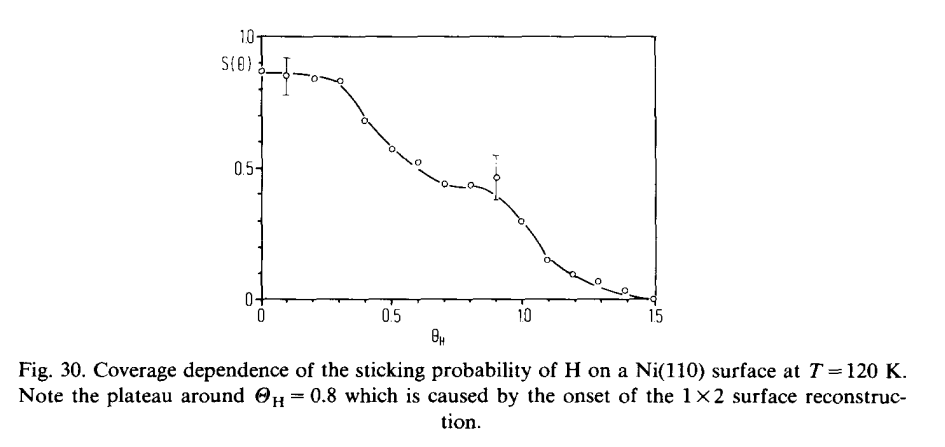
\includegraphics{Christmann_fig30.png}
\caption{Christmann\_fig30.png}
\end{figure}

    We just add that the dependence of \(s(\Theta)\) on the surface
crystallography is not a peculiar property of H adsorption. Dramatic
effects of this kind were also reported for oxygen adsorption on
\(Pt(100)\) surfaces (which are reconstructed in the clean state, with
\(s_0\) being small, and unreconstructed in the case of CO adsorption -
with \(s_0\) being at least an order of magnitude greater){[}256{]}.

    Остается добавить, что зависимость \(s(\Theta)\) от кристаллографии
поверхности не является специфическим свойством адсорбции H.
Драматические эффекты такого рода были также зарегистрированы для
адсорбции кислорода на поверхности \(Pt(100)\) (которая в чистом
состоянии реконструируется, и \(s_0\) становится малым, а в случае
адсорбции CO - не реконструируется, и \(s_0\) становится по крайней мере
на порядок больше){[}256{]}.

    Another very recent observation is concerned with \(H_2/D_2\) isotope
effects influencing the sticking probability at elevated H coverages on
Rh(110) surfaces. The experimental observations which are illustrated in
fig. 31 point to a pronounced dependence of \(s(\Theta)\) on the
long-range order of the adsorbate layer. H as well as D form among
others a \(1 \times 2-3H\) phase on Rh(110) at \(\Theta_H = 1.5\).
Interestingly, \(D_2\) adsorbs faster (higher \(s\)) into this phase
than \(H_2\), and one can only speculate on the reasons for this
behavior {[}103{]}. Undoubtedly, however, the better ordering of the
\(D_{ad}\) phases as compared to the \(H_{ad}\) phases improves the
efficiency of the sticking.

    Еще одно очень недавнее наблюдение касается изотопных эффектов
\(H_2/D_2\), влияющих на вероятность прилипания при повышенном покрытии
H на поверхности Rh(110). Экспериментальные наблюдения,
проиллюстрированные на рис. 31, указывают на ярко выраженную зависимость
\(s(\Theta)\) от дальнего порядка в слое адсорбата. H, а также D
образуют, в частности, фазу \(1 \times 2-3H\) на Rh(110) при
\(\Theta_H = 1.5\). Интересно, что \(D_2\) адсорбируется в эту фазу
быстрее (выше \(s\)), чем \(H_2\), и о причинах такого поведения можно
только гадать {[}103{]}. Несомненно, однако, что лучшее упорядочение фаз
\(D_{ad}\) по сравнению с фазами \(H_{ad}\) повышает эффективность
прилипания.

    \begin{figure}
\centering
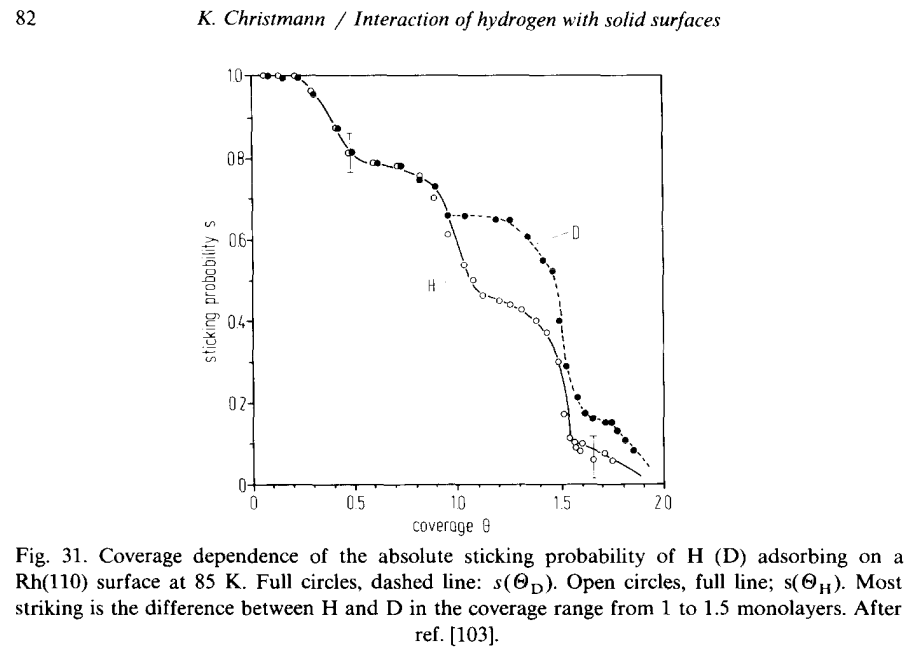
\includegraphics{Christmann_fig31.png}
\caption{Christmann\_fig31.png}
\end{figure}

    \section{3.5. Thermal desorption and the coverage dependence of the
desorption
kinetics}\label{thermal-desorption-and-the-coverage-dependence-of-the-desorption-kinetics}

    The reverse process to sticking and chemisorption is the desorption.
Once being trapped in any potential of the surface the particle (\(H_2\)
molecule or \(H\) atom) can only leave the surface again if it has
gained sufficient energy to reach the zero energy level. This is
equivalent to breaking the bond to the surface. In case of an existing
activation barrier in the adsorption path, \(\Delta E_{ad}^{*}\), this
must additionally be surmounted. The energetics of this process is
schematically illustrated in fig. 32.

    \section{3.5. Термическая десорбция и зависимость кинетики десорбции от
покрытия}\label{ux442ux435ux440ux43cux438ux447ux435ux441ux43aux430ux44f-ux434ux435ux441ux43eux440ux431ux446ux438ux44f-ux438-ux437ux430ux432ux438ux441ux438ux43cux43eux441ux442ux44c-ux43aux438ux43dux435ux442ux438ux43aux438-ux434ux435ux441ux43eux440ux431ux446ux438ux438-ux43eux442-ux43fux43eux43aux440ux44bux442ux438ux44f}

    Процессом, обратным прилипанию и хемосорбции, является десорбция.
Оказавшись в ловушке какого-либо потенциала поверхности, частица
(молекула \(H_2\) или атом \(H\)) может покинуть поверхность только в
том случае, если она приобрела энергию, достаточную для достижения
нулевого энергетического уровня. Это эквивалентно разрыву связи с
поверхностью. Если на пути адсорбции существует активационный барьер,
\(\Delta E_{ad}^{*}\), то его необходимо дополнительно преодолеть.
Энергетика этого процесса схематически показана на рис. 32.

    \begin{figure}
\centering
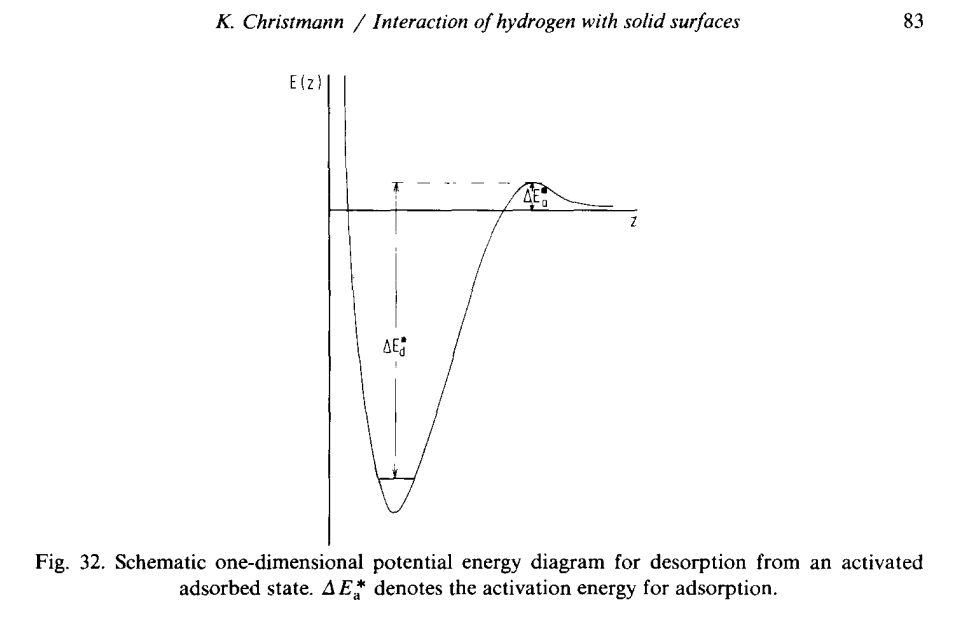
\includegraphics{Christmann_fig32.png}
\caption{Christmann\_fig32.png}
\end{figure}

    There are various ways in which the required energy can be supplied to
the bound particle, namely, by simply heating the substrate (whereby
phonon coupling is responsible for the energy transport) - this is the
thermal desorption or temperature programmed desorption (TPD) - or by
particle (mostly: electron) impact (EID) and by illuminating the surface
with electromagnetic radiation, e.g., laser light, whereby again thermal
effects must be distinguished from true photon-induced desorption
mechanisms in which the quanta excite the adsorbed particle directly. It
cannot be the intention of this article to enter any discussion of the
(certainly very interesting) mechanistic processes that are involved in
the excitation of a single bound adatom. Instead, we refer to the
excellent review articles which cover this field {[}257-259{]}. It is
just mentioned that, e.g., the laser-induced desorption is a technique
which is presently employed in a number of laboratories {[}258{]}.
Nevertheless we have to state that there is a general lack of
experimental data as compared to the research in the adsorption kinetics
or dynamics.

    Необходимая энергия может быть подведена к связанной частице различными
способами, а именно: простым нагреванием подложки (при этом фононная
связь отвечает за перенос энергии) - это термическая десорбция или
температурно запрограммированная десорбция (TPD) - или ударом частиц (в
основном электронов) (EID) и освещением поверхности электромагнитным
излучением, например, лазерным светом, при этом тепловые эффекты следует
отличать от истинных механизмов фотон-индуцированной десорбции, в
которых кванты возбуждают адсорбированную частицу напрямую. В задачи
данной статьи не входит обсуждение (безусловно, очень интересных)
механических процессов, которые вовлечены в возбуждение одного
связанного адатома. Вместо этого мы отсылаем вас к прекрасным обзорным
статьям, освещающим эту область {[}257-259{]}. Отметим лишь, что,
например, лазерно-индуцированная десорбция - это метод, который в
настоящее время используется в ряде лабораторий {[}258{]}. Тем не менее
приходится констатировать, что в целом наблюдается недостаток
экспериментальных данных по сравнению с исследованиями в области
кинетики или динамики адсорбции.

    Also, theoretical investigations are scarce. Again, we mention the work
of Kreuzer and Gortel {[}73,260{]} and the references given in their
work. This is why we confine ourselves to the process of thermal
desorption and here particularly on the kinetics of desorption of either
\(H_2\) molecules or \(H\) atoms from metal surfaces. Although the
thermal excitation process may be complicated as well, it is by far the
most commonly employed experimental technique and therefore a huge data
body exists. A description of thermal desorption spectroscopy in general
is given in numerous articles {[}257,259{]} to which we refer for any
further details. Nevertheless, it is deemed useful to present some
specific examples for \(H_2\) desorption spectra and to expand on the
analysis of the respective desorption kinetics.

    Теоретические исследования также немногочисленны. Мы снова упоминаем
работу Крейцера и Гортеля {[}73,260{]} и ссылки, приведенные в их
работе. Поэтому мы ограничимся рассмотрением процесса термической
десорбции и, в частности, кинетики десорбции молекул \(H_2\) или атомов
\(H\) с металлических поверхностей. Хотя процесс термического
возбуждения также может быть сложным, он, безусловно, является наиболее
часто используемой экспериментальной техникой. и поэтому существует
огромный массив данных. Описание спектроскопии термической десорбции в
целом приведено в многочисленных статьях {[}257,259{]}, к которым мы
отсылаем за любыми подробностями. Тем не менее, представляется
целесообразным привести несколько конкретных примеров для спектров
десорбции \(H_2\) и расширить анализ соответствующей кинетики десорбции.

    For dissociative adsorption (which is the rule with H on transition
metals) there is ample evidence that in most of the desorption reactions
the rate-limiting step is the recombination of separated adsorbed \(H\)
atoms to form the molecular transition state,
\(H_{2(ad)}^{{}_{+}^{+}}\). Normally this exhibits such a small binding
energy to the substrate that it desorbs immediately after its formation
at the temperatures usually employed in the TPD experiment: The
underlying reaction:

    Для диссоциативной адсорбции (что характерно для H на переходных
металлах) существует достаточно доказательств того, что в большинстве
реакций десорбции лимитирующим шагом является рекомбинация разделенных
адсорбированных атомов \(H\) с образованием молекулярного переходного
состояния, \(H_{2(ad)}^{{}_{+}^{+}}\). Обычно это состояние обладает
настолько малой энергией связи с субстратом, что десорбируется сразу
после своего образования при температурах, обычно используемых в
эксперименте TPD: Реакция, лежащая в основе:

    \(H_{ad} + H_{ad} \underset{k_{ad}}{\overset{k_d}{\leftrightarrows}} H_{2(ad)}^{{}_{+}^{+}}\overset{k_d^{\prime}}{\rightarrow}H_{2(g)}\)
(27)

    can be described by the rate expression:

    \(d\left[ H_{2(g)} \right] \big / dt = k_d \left[ H_{ad} \right]^2\)
(28)

    \(s_0\overset{-}c\left[ H_{2(g)} \right] = k_d \left[ H_{ad} \right]^2\)

    (apparent second-order desorption kinetics), whereby it is tacitly
assumed that \(k_{ad} \ll k_d\), and \(k_{d}^{\prime} \gg k_d\), under
the conditions of the experiment (high surface temperatures). \(k_d\)
then can be expressed as a normal rate constant:

    (кажущаяся кинетика десорбции второго порядка), при этом молчаливо
предполагается, что \(k_{ad} \ll k_d\), а \(k_{d}^{\prime} \gg k_d\), в
условиях эксперимента (высокие температуры поверхности). Тогда \(k_d\)
можно выразить как константу нормальной скорости:

    \(k_d = \nu_2 \left(\Theta\right) \, exp \left(-\frac{\Delta E^{*}_{d}\left(\Theta\right)}{kT} \right)\),

    in which \(\nu_2 \left(\Theta\right)\) denotes the pre-exponential
factor or ``frequency' factor and
\(\Delta E^{*}_{d}\left(\Theta\right)\) the activation barrier (which is
the depth of the chemisorption potential plus an eventual activation
barrier for adsorption, \(\Delta E^{*}_{ad}\)). Usually both \(\nu\) and
\(\Delta E^{*}_{d}\) depend on the adsorbate concentration, \(\Theta\).
According to eq.(28) \(\nu_2 \left(\Theta\right)\) has the dimension
\([cm^2/s \cdot H-atom]\) for a true second-order rate process.

    где \(\nu_2 \left(\Theta\right)\) обозначает предэкспоненциальный фактор
или «частотный» фактор, а \(\Delta E^{*}_{d}\left(\Theta\right)\) -
активационный барьер (который представляет собой глубину
хемосорбционного потенциала плюс возможный активационный барьер для
адсорбции, \(\Delta E^{*}_{ad}\)). Обычно и \(\nu\), и
\(\Delta E^{*}_{d}\) зависят от концентрации адсорбата, \(\Theta\).
Согласно уравнению (28) \(\nu_2 \left(\Theta\right)\) имеет размерность
\([cm^2/s \cdot H-atom]\) для истинного процесса второго порядка.

    A more quantitative interpretation of the frequency factor may be
obtained within the framework of transition state theory (TST) {[}261{]}
whereby refinements of this theory regarding the thermal desorption have
been made by Garrison et al. {[}262{]}. It can be shown that, for the
zero coverage limit, the pre-exponential factor is obtained by equating
the rates of adsorption and desorption, \(r_{ad}\) and \(r_{des}\)
(which corresponds to the adsorption-desorption equilibrium):

    Более количественная интерпретация частотного фактора может быть
получена в рамках теории переходных состояний (ТПС) {[}261{]}, уточнения
которой в отношении термической десорбции были сделаны Гаррисоном и др
{[}262{]}. Можно показать, что для предела нулевого покрытия
предэкспоненциальный фактор получается приравниванием скоростей
адсорбции и десорбции, \(r_{ad}\) и \(r_{des}\) (что соответствует
адсорбционно-десорбционному равновесию):

    \(s_0\overset{-}c\left[ H_{2(g)} \right] = k_d \left[ H_{ad} \right]^2\)

    \(s_0\overset{-}c n_g = k_d n_{ad}^2\)

    \(s_0\overset{-}c n_g = \nu_2 \, exp \left(-\frac{\Delta E^{*}_{d}}{kT} \right) n_{ad}^2\)

    \(s_0\overset{-}c n_g \, exp \left(\frac{\Delta E^{*}_{d}}{kT} \right) = \nu_2 n_{ad}^2\)

    \(s_0\overset{-}c \frac{n_g}{n_{ad}^2} \, exp \left(\frac{\Delta E^{*}_{d}}{kT} \right) = \nu_2\)

    \(\nu_2 = s_0\overset{-}c \frac{n_g}{n_{ad}^2} \, exp \left(\frac{\Delta E^{*}_{d}}{kT} \right)\),
(30)

    in which \(\overset{-}c\) denotes the mean velocity \([cm \,\,s^{-1}]\)
and \(n_g\) the number of \(H_2\) gas molecules per unit volume
\([cm^{-3}]\). \(n_{ad}\) stands for the number of \(H\) atoms adsorbed
per unit area \([cm^{-2}]\) of the surface.

    где \(\overset{-}c\) обозначает среднюю скорость \([см\,\,с^{-1}]\),
\(n_g\) - число молекул газа \(H_2\) на единицу объема \([см^{-3}]\).
\(n_{ad}\) обозначает число атомов \(H\), адсорбированных на единицу
площади \([см^{-2}]\) поверхности.

    \begin{tcolorbox}[breakable, size=fbox, boxrule=1pt, pad at break*=1mm,colback=cellbackground, colframe=cellborder]
\prompt{In}{incolor}{ }{\boxspacing}
\begin{Verbatim}[commandchars=\\\{\}]

\end{Verbatim}
\end{tcolorbox}

    Using statistical mechanics the ratio \(n_g/n_{ad}\) for the equilibrium

\(H_{2(g)} + 2 * {\rightarrow} 2 H_{ad}\) (31)

may be written as

\(\frac{n_g}{n_{ad}^2} = \frac{f_g f_{s,0}^2}{f_{ad}^2 f_{s,ad}^2} \, exp \left(-\frac{\Delta E^{*}_{d}}{kT} \right)\)
(32)

for the case of non-activated adsorption
(\(\Delta E^{*}_{d} = \Delta E_{ad}\)) and the limit of small coverages
and non-interacting particles. \(f_g\) is the molecular partition
function per \(cm^2\) of \(H_2\) gas \((2 \pi m k T/h^3)^{3/2}\) and
\(f_{ad}\) that for adsorbed \(H\) atoms per \(cm^2\) of the surface
area. \(f_{ad}\) is given by the total number provided by the surface,
\(N_s\), times the complete partition function of the single adsorbed
\(H\) atom. \(f_{s,0}\) is the molecular partition function of the bare
surface (except for contributions from the motions of the adsorbate).
The partition functions \(f_{s,0}\), \(f_{s,ad}\) and \(f_{ad}\) can be
combined to yield:

\(f_{ad}^{\prime} = f_{ad} f_{s,ad}/f_{s,0}\) (33)

and we obtain, by relating eqs. (30), (32) and (33) for the
pre-exponential factor

\(\nu_2 = s_0 \overset{-}c f_g/f_{ad}^{\prime}\). (34)

    Используя статистическую механику, можно определить соотношение
\(n_g/n_{ad}\) для равновесия

\(H_{2(g)} + 2 * {\rightarrow} 2 H_{ad}\) (31)

может быть записано как

\(\frac{n_g}{n_{ad}^2} = \frac{f_g f_{s,0}^2}{f_{ad}^2 f_{s,ad}^2} \, exp \left(-\frac{\Delta E^{*}_{d}}{kT} \right)\)
(32)

для случая неактивированной адсорбции
(\(\Delta E^{*}_{d} = \Delta E_{ad}\)) и предела малых покрытий и
невзаимодействующих частиц. \(f_g\) - функция молекулярного разделения
на \(см^2\) газа \(H_2\) \((2 \pi m k T/h^3)^{3/2}\), а \(f_{ad}\) - для
адсорбированных атомов \(H\) на \(см^2\) площади поверхности. \(f_{ad}\)
определяется общим числом, обеспечиваемым поверхностью, \(N_s\),
умноженным на полную функцию разделения одного адсорбированного атома
\(H\). \(f_{s,0}\) - молекулярная функция разделения голой поверхности
(за исключением вклада от движений адсорбата). Функции разделения
\(f_{s,0}\), \(f_{s,ad}\) и \(f_{ad}\) могут быть объединены, чтобы
получить:

\(f_{ad}^{\prime} = f_{ad} f_{s,ad}/f_{s,0}\) (33)

и мы получаем, связав уравнения (30), (32) и (33) для
предэкспоненциального коэффициента

\(\nu_2 = s_0 \overset{-}c f_g/f_{ad}^{\prime}\). (34)

    \begin{tcolorbox}[breakable, size=fbox, boxrule=1pt, pad at break*=1mm,colback=cellbackground, colframe=cellborder]
\prompt{In}{incolor}{ }{\boxspacing}
\begin{Verbatim}[commandchars=\\\{\}]

\end{Verbatim}
\end{tcolorbox}

    Experimentally, a second-order rate process is characterized by a
continuous shift of the temperature-programmed desorption (TPD) maximum
towards lower temperatures with increasing coverage. A second-order
desorption reaction has been reported so far for a variety of
metal-hydrogen systems, for example for the high-energy binding states
of \(H\)

on \(Ni(111)\) {[}50,67{]} and on \(Ni(100)\) {[}56{]},

on \(Pd(110)\) {[}68{]} and (111) {[}266{]},

\(H\) desorbing from

\(Rh(111)\) {[}243{]},

\(Pt(100)\) {[}267{]},

\(Fe(110)\) {[}159{]},

\(Ru(0001)\) {[}113{]} or

\(W(110)\) {[}268{]}.

An example for a typical second order TPD spectrum is given in fig. 33
which was obtained with \(H\) on \(Pt(111)\) {[}158{]}.

    Экспериментально процесс скорости второго порядка характеризуется
непрерывным смещением максимума температурно-программированной десорбции
(ТПД) в сторону более низких температур с увеличением покрытия. Реакция
десорбции второго порядка была зарегистрирована для различных систем
металл-водород, например, для высокоэнергетических связанных состояний
\(H\)

на \(Ni(111)\) {[}50,67{]} и на \(Ni(100)\) {[}56{]},

на \(Pd(110)\) {[}68{]} и (111) {[}266{]},

десорбция \(H\) из

\(Rh(111)\) {[}243{]},

\(Pt(100)\) {[}267{]},

\(Fe(110)\) {[}159{]},

\(Ru(0001)\) {[}113{]} или

\(W(110)\) {[}268{]}.

Пример типичного спектра TPD второго порядка приведен на рис. 33,
который был получен с \(H\) на \(Pt(111)\) {[}158{]}.

    \begin{figure}
\centering
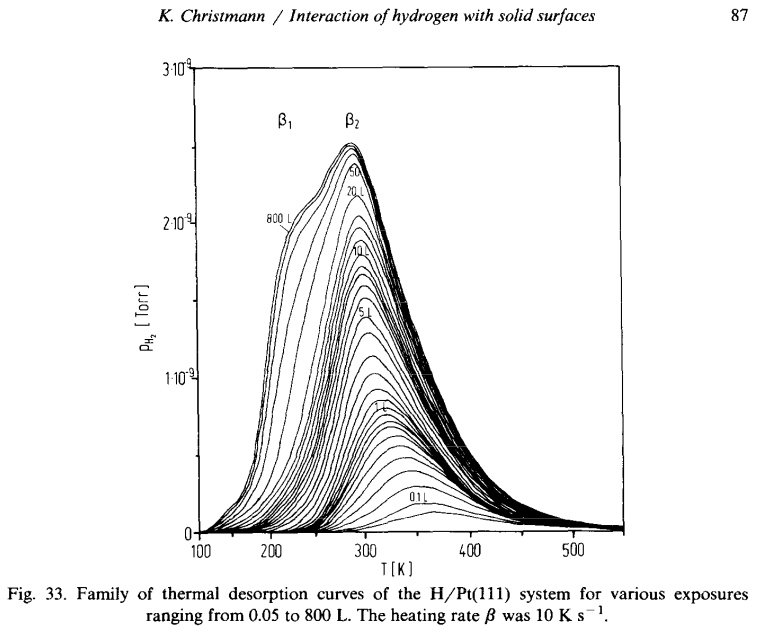
\includegraphics{Christmann_fig33.png}
\caption{Christmann\_fig33.png}
\end{figure}

    However, there are quite many cases in which true second-order
desorption kinetics is difficult to establish. It may turn out that the
TPD data can be interpreted also in terms of a first-order rate process.
An almost ``classical'' example is provided by the system \(H\) on
\(Pt(111)\) which was first investigated by Lang et al. {[}269{]} who
claimed that there was no adsorption at all. Later reinvestigations by
Lu and Rye {[}270{]}, by Christmann et al. {[}158{]}, by Collins and
Spicer {[}271{]} or McCabe and Schmidt {[}272{]} clearly revealed that
\(H\) chemisorption was indeed occurring, however, there were
considerable discrepancies with respect to the desorption kinetics, the
value of the frequency factor and the height of the activation energy
for desorption.

    Однако существует довольно много случаев, когда истинную кинетику
десорбции второго порядка установить сложно. Может оказаться, что данные
TPD можно интерпретировать и в терминах процесса первого порядка. Почти
«классическим» примером является система \(H\) на \(Pt(111)\), которая
впервые была исследована Лангом и другими {[}269{]}, которые утверждали,
что адсорбция вообще не происходит. Более поздние повторные
исследования, проведенные Лу и Райе {[}270{]}, Кристманном и другими
{[}158{]}, Коллинзом и Спайсером {[}271{]} или МакКейбом и Шмидтом
{[}272{]}, ясно показали, что хемосорбция \(H\) действительно имеет
место, однако в отношении кинетики десорбции, значения частотного
фактора и высоты энергии активации десорбции наблюдались значительные
расхождения.

    Whilst the authors of ref. {[}158{]} claimed a second-order desorption
and a very low pre-exponential {[}265{]} as well as a low activation
energy for desorption McCabe and Schmidt considered a first-order
process with a much higher frequency factor and a higher activation
energy \(\Delta E^{*}_{d}\). This problem persisted until 1981 when
molecular beam work in the group of Comsa revealed strong evidence for a
higher activation energy for desorption which in turn makes a
first-order order pre-exponential more likely {[}273{]}. It also turned
out that the concentration of surface defects was crucially influencing
the adsorption/desorption kinetics {[}60{]}.

    В то время как авторы работы {[}158{]} утверждали, что десорбция идет по
второму порядку и имеет очень низкий предэкспоненциал {[}265{]}, а также
низкую энергию активации для десорбции. {[}158{]} утверждали о десорбции
второго порядка и очень низком предэкспоненциале {[}265{]}, а также о
низкой энергии активации десорбции МакКейб и Шмидт считали процесс
первого порядка с гораздо более высоким частотным фактором и более
высокой энергией активации \(\Delta E^{*}_{d}\). Эта проблема
сохранялась до 1981 года, когда в результате работы с молекулярным
пучком в группе Комса были получены убедительные доказательства более
высокой энергии активации десорбции, что, в свою очередь, делает более
вероятным предэкспоненциальный порядок первого порядка {[}273{]}.
Оказалось также, что концентрация поверхностных дефектов оказывает
решающее влияние на кинетику адсорбции/десорбции {[}60{]}.

    Whereas a second-order desorption is often observed for the high-energy
binding states a first-order desorption kinetics has occasionally been
reported, when additional low-energy binding states become populated.
Examples are the \(\beta_1\) state for \(H\) on \(Ni(110)\)
{[}230,231{]}, the \(\alpha_1\) and \(\alpha_2\) states for Rh(110)
{[}70{]}, and the \(\alpha_1\) and \(\alpha_2\) states for \(H\) on
\(Pd(110)\) {[}68{]}. This first-order kinetics

    В то время как для высокоэнергетических состояний связывания часто
наблюдается десорбция второго порядка, иногда сообщается о кинетике
десорбции первого порядка, когда заселяются дополнительные
низкоэнергетические состояния связывания. Примерами являются состояние
\(\beta_1\) для \(H\) на \(Ni(110)\) {[}230,231{]}, состояния
\(\alpha_1\) и \(\alpha_2\) для Rh(110) {[}70{]}, состояния \(\alpha_1\)
и \(\alpha_2\) для \(H\) на \(Pd(110)\) {[}68{]}. Эта кинетика первого
порядка

    \(H_{ad} + H_{ad} \underset{k_{ad}}{\overset{k_d}{\leftrightarrows}} H_{2(ad)}^{{}_{+}^{+}}\overset{k_d^{\prime}}{\rightarrow}H_{2(g)}\)

    \(d\left[ H_{2(g)} \right] \big / dt = k_d^{\prime} \left[ H_{2(ad)}^{{}_{+}^{+}} \right]\)
(39)

    \(s_0\overset{-}c\left[ H_{2(g)} \right] = k_d^{\prime} \left[ H_{2(ad)}^{{}_{+}^{+}} \right]\)

    \(s_0\overset{-}c n_g = k_d^{\prime} \frac{n_{ad}^{H}}{2} = k_d^{\prime} {n_{ad}^{H_2}}\)

    with

    \(k_d^{\prime} = \nu_1 \left(\Theta\right) \, exp \left(-\frac{\Delta E^{*}_{d}\left(\Theta\right)}{kT} \right)\)
(40)

    and

    \(\nu_1 = \kappa_d \frac{k T}{h} \frac{f_{d}^{{}_{+}^{+}}}{f_{ad}} \,\,\, [s^{-1}]\)
(40)

    would suggest an associative desorption mechanism in which the
desorptive removal of an already formed \(H_{2(ad)}^{{}_{+}^{+}}\),
entity would at least formally be rate-limiting
(\(k_{d}^{\prime} \ll k_d\) in eq. (27)).

    \begin{tcolorbox}[breakable, size=fbox, boxrule=1pt, pad at break*=1mm,colback=cellbackground, colframe=cellborder]
\prompt{In}{incolor}{ }{\boxspacing}
\begin{Verbatim}[commandchars=\\\{\}]

\end{Verbatim}
\end{tcolorbox}

    \(s_0\overset{-}c n_g = \nu_1 \, exp \left(-\frac{\Delta E^{*}_{d}}{kT} \right) \frac{n_{ad}^{H}}{2}\)

    \(s_0\overset{-}c n_g \, exp \left(\frac{\Delta E^{*}_{d}}{kT} \right) = \nu_1 \frac{n_{ad}^{H}}{2}\)

    \(s_0\overset{-}c \frac{2 n_g}{n_{ad}^{H}} \, exp \left(\frac{\Delta E^{*}_{d}}{kT} \right) = \nu_1\)

    \(\nu_1 = s_0\overset{-}c \frac{n_g}{n_{ad}^{H}/2} \, exp \left(\frac{\Delta E^{*}_{d}}{kT} \right)\)

    \begin{tcolorbox}[breakable, size=fbox, boxrule=1pt, pad at break*=1mm,colback=cellbackground, colframe=cellborder]
\prompt{In}{incolor}{ }{\boxspacing}
\begin{Verbatim}[commandchars=\\\{\}]

\end{Verbatim}
\end{tcolorbox}

    With many of the first-order systems cited above, however, there is no
other evidence for such a mechanism and one must caution that either
coverage-dependent lateral interaction forces or structural phase
changes within the adsorbed layer during the temperature program are
responsible for those ``pseudo-first-order'' kinetics. Indeed, for the
system \(Rh(11O)/H\) {[}70{]} a careful inspection of the TPD spectra
revealed small peak shifts indicating a possible slight fractional-order
desorption kinetics. This could for example be caused by preferential
desorption from the ends of linear H chains which are formed along the
troughs of that (110) surface. Furthermore, with \(Pd(11O)/H\) and
\(Ni(11O)/H\) clearly surface reconstruction phenomena and/or population
of subsurface sites {[}275{]} are accompanying the adsorption which
likewise modify the desorption kinetics.

    Однако для многих систем первого порядка, приведенных выше, нет других
доказательств такого механизма, и следует предположить, что либо силы
латерального взаимодействия, зависящие от покрытия, либо структурные
фазовые изменения в адсорбированном слое во время температурной
программы ответственны за эту «псевдопервопорядковую» кинетику.
Действительно, для системы \(Rh(11O)/H\) {[}70{]} тщательное изучение
спектров TPD выявило небольшие сдвиги пиков, указывающие на возможную
незначительную кинетику десорбции дробного порядка. Это может быть
вызвано, например, преимущественной десорбцией с концов линейных цепочек
H, которые образуются вдоль впадин этой (110) поверхности. Кроме того, в
случае \(Pd(11O)/H\) и \(Ni(11O)/H\) адсорбции явно сопутствуют явления
реконструкции поверхности и/или заселения приповерхностных участков
{[}275{]}, которые также изменяют кинетику десорбции.

    \begin{tcolorbox}[breakable, size=fbox, boxrule=1pt, pad at break*=1mm,colback=cellbackground, colframe=cellborder]
\prompt{In}{incolor}{ }{\boxspacing}
\begin{Verbatim}[commandchars=\\\{\}]

\end{Verbatim}
\end{tcolorbox}

    Other complications, as mentioned before, may arise from the existence
of precursor states in the desorption path which, according to the
``detailed balancing'', should modify the thermal desorption traces
considerably, as long as the temperatures are low enough to ensure a
noticeable population of these states. Shanabarger {[}276,277{]} studied
the adsorption/desorption on iron and nickel films and interpreted his
kinetic results in terms of a precursor state model, that is, he
regarded the formation of a molecular precursor state as the
rate-limiting step in the desorption channel. Later King {[}235{]} and
Gorte and Schmidt {[}236{]} subjected the precursor influence to a more
rigorous treatment and showed that the desorption rate must be
significantly modified.

    Другие осложнения, как уже говорилось, могут возникнуть из-за
существования на пути десорбции состояний-предшественников, которые,
согласно «детальному балансу», должны значительно модифицировать следы
термической десорбции, если только температуры достаточно низки, чтобы
обеспечить заметную заселенность этих состояний. Шанабаргер
{[}276,277{]} изучал адсорбцию/десорбцию на пленках железа и никеля и
интерпретировал свои кинетические результаты в терминах модели
состояния-предшественника, то есть рассматривал образование
молекулярного состояния-предшественника как лимитирующий по скорости
этап в канале десорбции. Позже Кинг {[}235{]} и Горте и Шмидт {[}236{]}
подвергли влияние прекурсора более строгой обработке и показали, что
скорость десорбции должна быть значительно изменена.

    More recent work on the same subject by Alnot and King {[}278{]},
Cassuto and King {[}238{]} and Alnot and Cassuto {[}279{]} led to an
analytical expression for the desorption rate which contains only
probability functions for adsorption and desorption from the precursor
and for the surface migration in the precursor.

The advantage of the formula by Cassuto and King {[}238{]} is the fairly
general applicability. For more details about how precursor states can
alter the desorption kinetics we recommend the review paper by Morris et
al. {[}78{]} for further reading.

    Более поздние работы по этому вопросу Алнота и Кинга {[}278{]}, Кассуто
и Кинга {[}238{]} и Алнота и Кассуто {[}279{]} привели к аналитическому
выражению для скорости десорбции, которое содержит только функции
вероятности для адсорбции и десорбции из прекурсора и для миграции
поверхности в прекурсоре.

Преимуществом формулы Кассуто и Кинга {[}238{]} является ее достаточно
общая применимость. Для получения более подробной информации о том, как
состояния прекурсора могут изменять кинетику десорбции, мы рекомендуем
обзорную статью Морриса и других {[}78{]} для дальнейшего чтения.

    \begin{tcolorbox}[breakable, size=fbox, boxrule=1pt, pad at break*=1mm,colback=cellbackground, colframe=cellborder]
\prompt{In}{incolor}{ }{\boxspacing}
\begin{Verbatim}[commandchars=\\\{\}]

\end{Verbatim}
\end{tcolorbox}

    In principle, a state selective desorption spectroscopy is required to
disentangle the details of the desorption process, for example, the
various atomic or molecular excitations (translation, rotation,
vibration).

    В принципе, для расчленения деталей процесса десорбции, например,
различных атомных или молекулярных возбуждений (трансляция, вращение,
вибрация), необходима спектроскопия селективной десорбции по состоянию.

    \begin{tcolorbox}[breakable, size=fbox, boxrule=1pt, pad at break*=1mm,colback=cellbackground, colframe=cellborder]
\prompt{In}{incolor}{ }{\boxspacing}
\begin{Verbatim}[commandchars=\\\{\}]

\end{Verbatim}
\end{tcolorbox}

    An important contribution to the desorption dynamics of hydrogen from
surfaces was, among others, published by Kubiak et al. {[}274{]} who
studied the rotational and vibrational distribution of \(H_2\) and
\(D_2\) recombinatively desorbing from clean Cu(110) and (111) surfaces
following atomic permeation through the Cu crystals at \(T_s\) = 850 K
and 960 K.

Multiphonon excitation (ionization) was combined with time-of-flight
mass spectroscopy. The rotational distributions of the desorbing \(H_2\)
(\(D_2\)) molecules were found to be non-Boltzmann and showed mean
rotational energies which where 80\%-90\% of the surface temperature,
\(T_s\), regardless of the isotope and of the surface orientation.

In contrast, the vibrational population ratio as given by the fraction
of molecules with quantum numbers \(v_1\) : \(v_0\). was found
approximately a factor of 100 greater than the ratio predicted by
Boltzmann statistics at \(T_s\).

The conclusion was that detailed balance arguments applied to the
vibrational distributions measured in recombinative desorption are not
suited to predict correctly the dissociative adsorption probability as a
function of vibration: It is concluded that these two processes are
dynamically different at least for the \(Cu(110)\) and \(Cu(111)/H\)
systems.

    Важный вклад в динамику десорбции водорода с поверхностей внесли, в
частности, работы Кубиака и других {[}274{]}, которые изучали
вращательное и колебательное распределение \(H_2\) и \(D_2\),
рекомбинационно десорбирующихся с чистых поверхностей Cu(110) и (111)
после атомного проникновения через кристаллы Cu при \(T_s\) = 850 K и
960 K.

Многофононное возбуждение (ионизация) сочеталось с времяпролетной
масс-спектроскопией. Вращательные распределения десорбирующихся молекул
\(H_2\) (\(D_2\)) оказались небольцмановскими и показали средние энергии
вращения, составляющие 80-90 \% от температуры поверхности, \(T_s\),
независимо от изотопа и ориентации поверхности.

Напротив, отношение колебательной населенности, определяемое долей
молекул с квантовыми числами \(v_1\) : \(v_0\), оказалось примерно в 100
раз больше, чем отношение, предсказанное статистикой Больцмана при
\(T_s\).

В результате был сделан вывод, что детальные балансовые аргументы,
примененные к колебательным распределениям, измеренным при
рекомбинационной десорбции, не подходят для правильного предсказания
вероятности диссоциативной адсорбции как функции колебаний: Сделан
вывод, что эти два процесса динамически различны, по крайней мере, для
систем \(Cu(110)\) и \(Cu(111)/H\).

    \begin{tcolorbox}[breakable, size=fbox, boxrule=1pt, pad at break*=1mm,colback=cellbackground, colframe=cellborder]
\prompt{In}{incolor}{ }{\boxspacing}
\begin{Verbatim}[commandchars=\\\{\}]

\end{Verbatim}
\end{tcolorbox}

    As in the case of the adsorption (cf. section 3.4) the lateral
interaction forces can modify the desorption kinetics to a great extent.
This is illustrated by fig. 34 which is taken from Adams' work {[}246{]}
and shows how the magnitude of the nearest neighbor repulsive energy
\(\omega\) can really alter a thermal desorption spectrum. Goymour and
King {[}280{]} used the quasi-chemical approximation to model the effect
of repulsive lateral interactions on second-order thermal desorption.
The presence of these interactions lowers the heat of adsorption (and
hence \(E_d^{\prime}\)) as the coverage increases, and the frequency
factor takes on a complicated coverage dependence which, among others,
contains the interaction energy, \(\omega\) and its coverage dependence.

    Как и в случае адсорбции (см. раздел 3.4), силы латерального
взаимодействия могут в значительной степени изменять кинетику десорбции.
Это иллюстрирует рис. 34, взятый из работы Адамса {[}246{]} и
показывающий, как величина энергии отталкивания ближайшего соседа
\(\omega\) может действительно изменить спектр тепловой десорбции.
Гоймур и Кинг {[}280{]} использовали квазихимическое приближение для
моделирования влияния отталкивающих латеральных взаимодействий на
тепловую десорбцию второго порядка. Наличие этих взаимодействий снижает
теплоту адсорбции (и, следовательно, \(E_d^{\prime}\)) по мере
увеличения покрытия, и частотный фактор приобретает сложную зависимость
от покрытия, которая, помимо прочего, содержит энергию взаимодействия
\(\omega\) и ее зависимость от покрытия.

    \begin{figure}
\centering
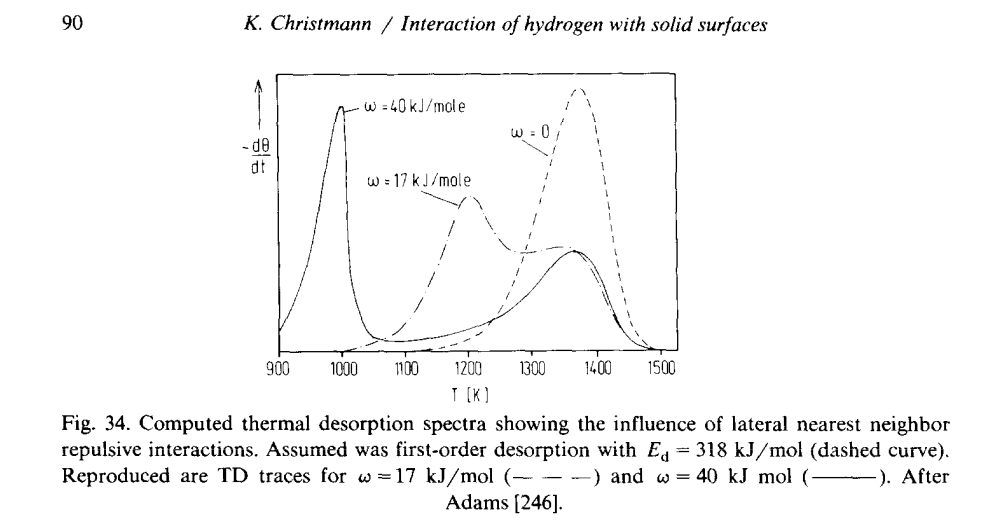
\includegraphics{Christmann_fig34.png}
\caption{Christmann\_fig34.png}
\end{figure}

    However, for the sake of all the complications mentioned above it seems
to be not very wise to rely on TPD analysis alone to extract the
information about sign and magnitude of lateral interactions. More
promising is certainly an investigation of the long-range order effects
which can be observed quite frequently with interacting particles on a
surface.

    Однако, учитывая все вышеперечисленные сложности, полагаться только на
TPD-анализ для получения информации о знаке и величине латеральных
взаимодействий представляется не очень разумным. Более перспективным
представляется исследование дальнодействующих эффектов дальнего порядка,
которые довольно часто наблюдаются при взаимодействии частиц на
поверхности.

    \section{Никель водородный
кольцар}\label{ux43dux438ux43aux435ux43bux44c-ux432ux43eux434ux43eux440ux43eux434ux43dux44bux439-ux43aux43eux43bux44cux446ux430ux440}

    предполагаемая схема водородно никелевого кольцара, построенная исходя
из информации изложенной выше

    \begin{figure}
\centering
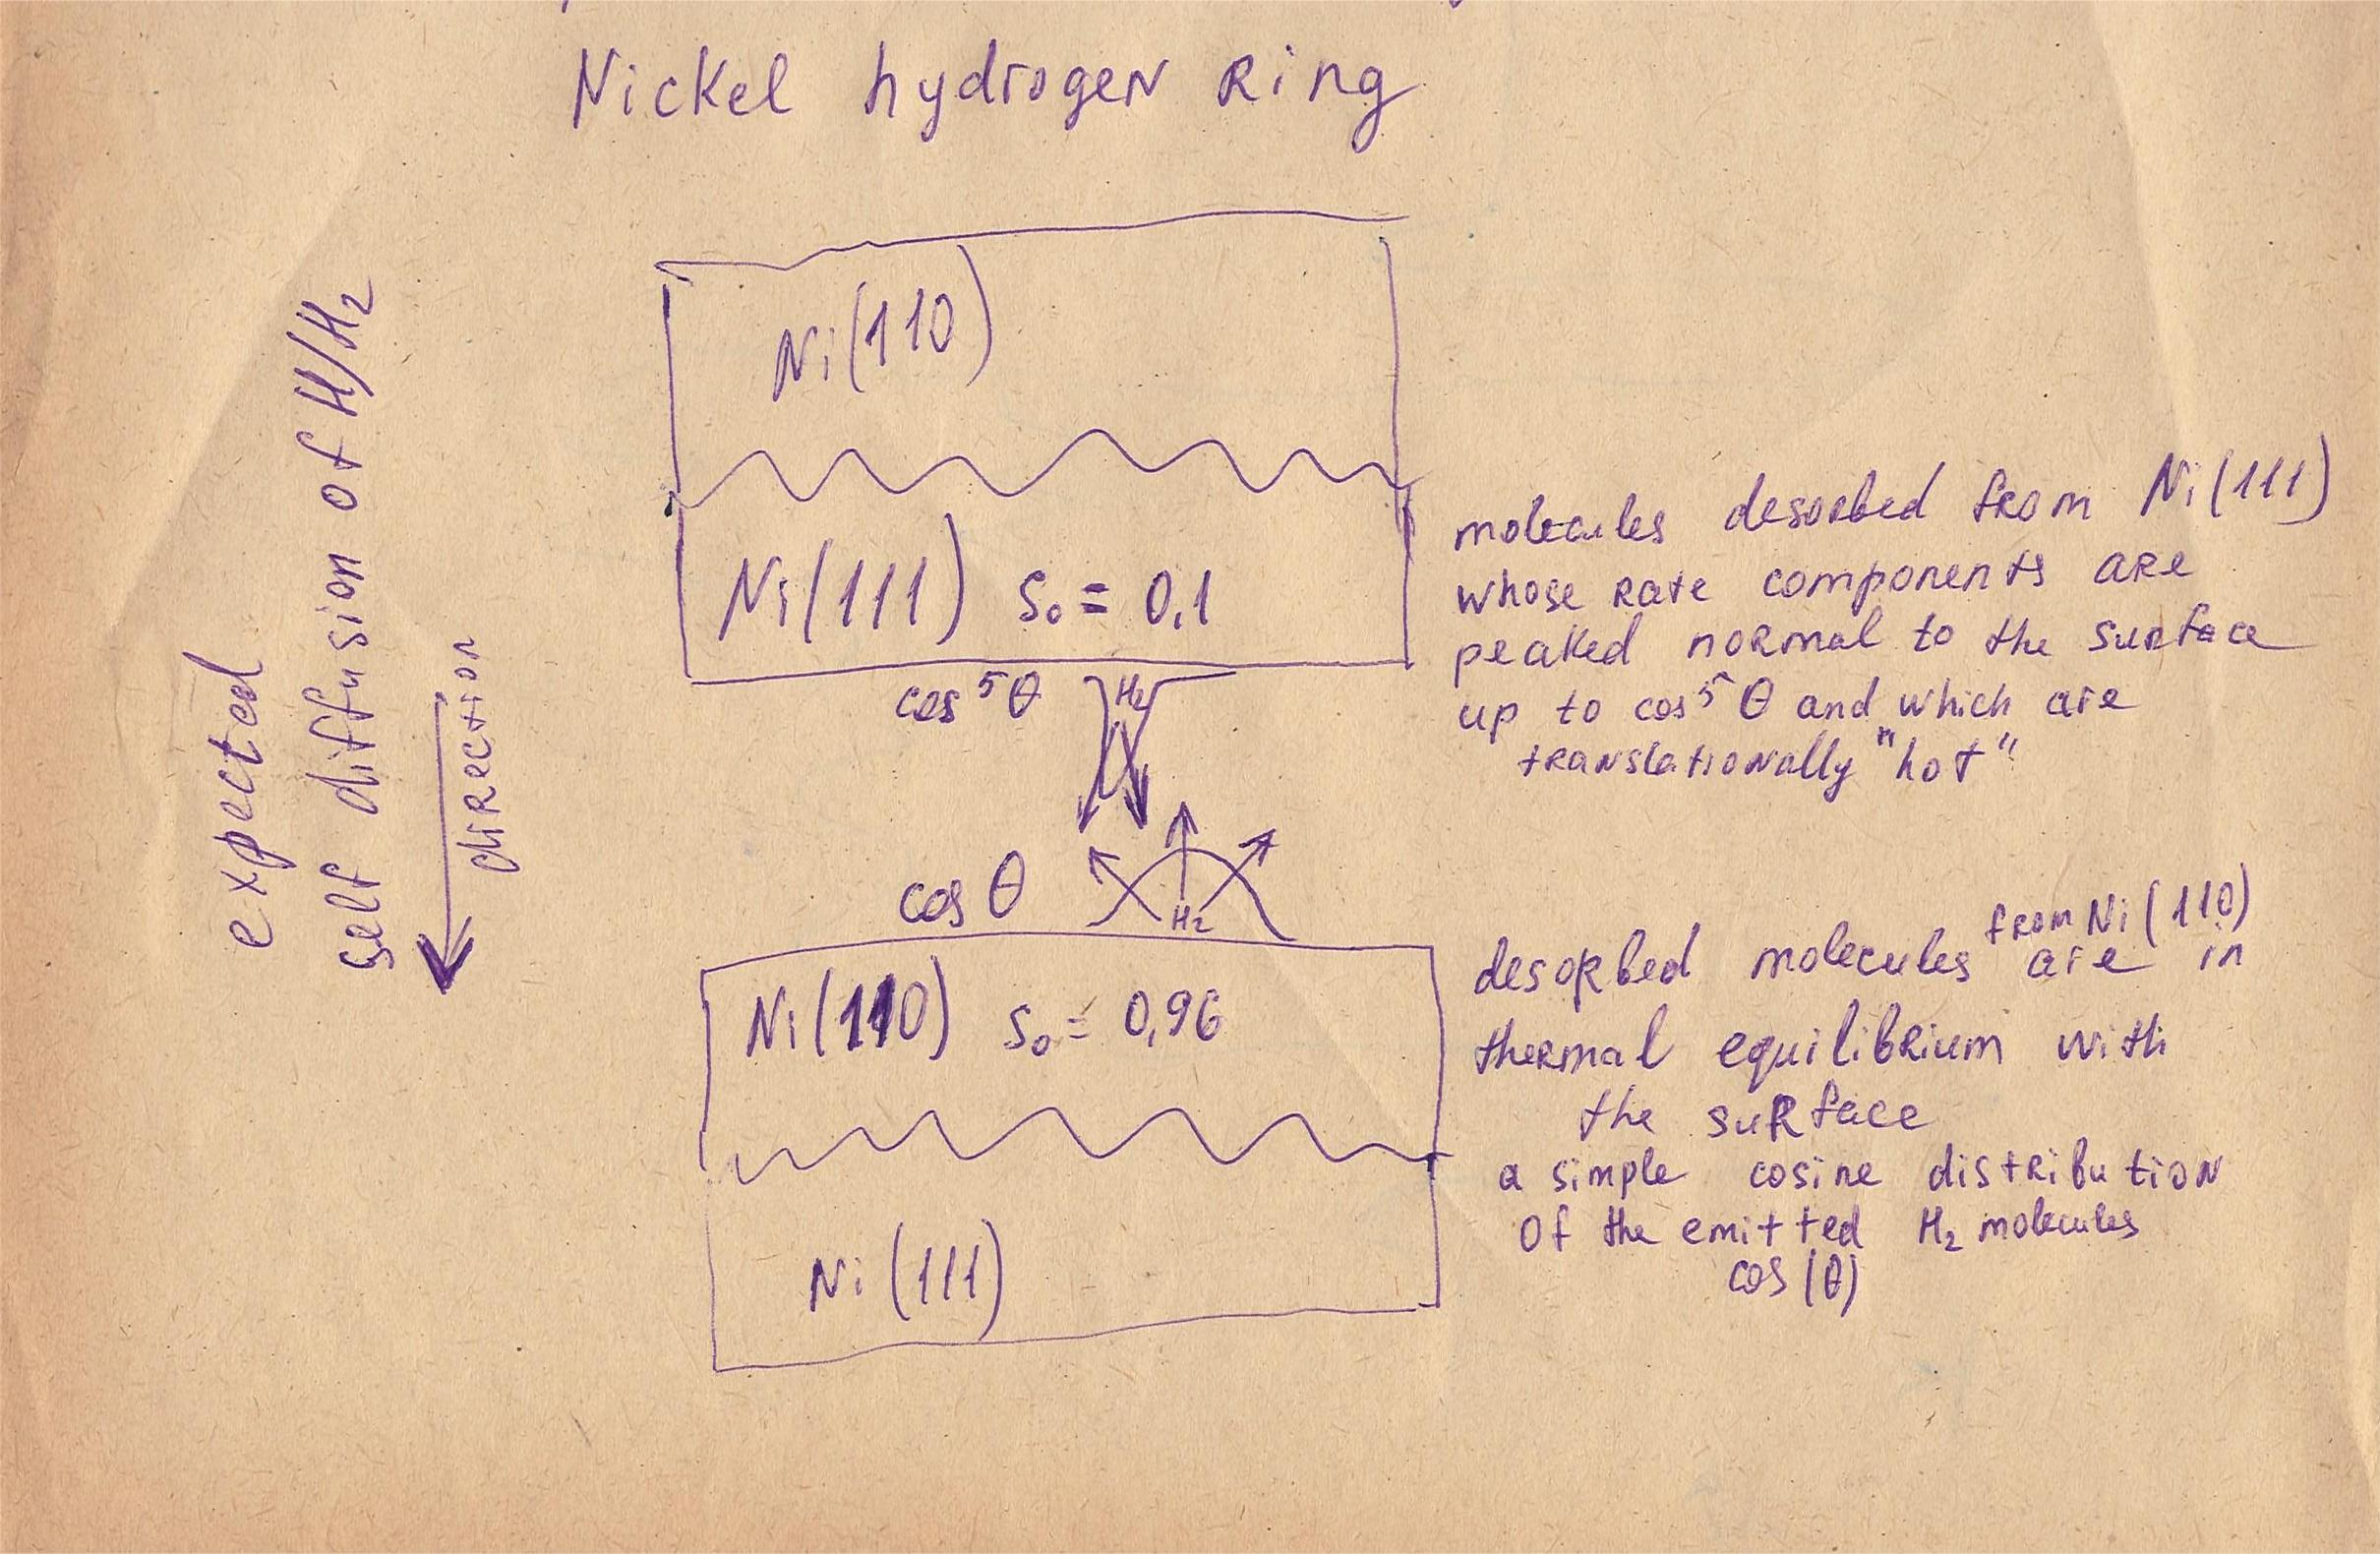
\includegraphics{Ni_H2_ring.jpg}
\caption{Ni\_H2\_ring.jpg}
\end{figure}

    Выходная часть мембраны состоит из Ni(111) или Ni(100) которая имеет
весьма низкий коэффициент прилипания \(s_0 = 0.1\), угловое
распределение десорбирующихся молекул водорода имеет весьма острый вид
\(cos^5 \theta\) при том что десорбирующиеся молекулы трансляционно
"горячие" и направлены преимущественно перпендикулярно поверхности
мембраны.

Входная часть мембраны состоит из Ni(110), имеющая весьма высокий
коэффициент прилипания \(s_0 = 0.96\), десорбирующиеся молекулы имеют
угловое распределение \(cos \theta\) и находятся в состоянии теплового
равновесия с температурой поверхности входной мембраны.

Ожидаемое направление самопроизвольной диффузии от выходной поверхности
мембраны к входной.

    Объяснение принципа работы водородно никелевого кольцара состоит в
частности в том, что при достаточно малом зазоре и достаточно малой
концентрации газообразного водорода в газовой фазе как раз и будет
отклонение от принципа детального равновесия, если рассмотреть
распределение молекул водорода по углу \(\theta\) направления движения
относительно поверхности. Вследствие того, что поверхность Ni(110)
десорбирует молекулы с более широким распределением по углам
(\(sin \theta\)), чем поверхность Ni(111), которая десорбирует молекулы
водорода в обратном направлении, но с более острым угловым
распределением.

Предположим что концентрация молекул в газовой фазе настолько мала, что
столкновениями молекул водорода друг с другом в газовой фазе
маловероятны. То есть если ширина промежутка меньше длины свободного
пробега молекул.

Отсюда следует, что в газовом промежутке ожидается отклонение от
принципа детального равновесия благодаря тому что для наклонных
направлений к поверхности количество молекул десорбированных по рисунку
вверх будет больше, чем десорбированных по рисунку вниз, а для
нормальных направлений к поверхности количество молекул десорбированных
по рисунку вниз будет больше, чем количество молекул, десорбированных по
рисунку вверх.

Далее вследствие различия вероятности прилипания вероятность того, что
нормально направленные к поверхности молекулы, которые были
десорбированы из верхней по рисунку поверхности (которые к тому же ещё и
трансляционно "горячие") и долетели нижней по рисунку поверхности,
вероятность их поглощения на нижней по рисунку поверхности Ni (110)
достаточно высока вследствие значения коэффициента прилипания
\(s_0 = 0.96\).

В противоположность этому вероятность того, что нормально направленные
молекулы которые были десорбированы с нижней по рисунку поверхности
Ni(110), (которые уже трансляционно не "горячие", а равновесно
уравновешенные с температурой поверхности десорбирования) и которые
долетели до верхней по рисунку поверхности Ni(111), так вот вероятность
их адсорбирования уже низкая из за: 1) их относительно меньшей
кинетической энергии 2) из-за весьма низкого коэффициента прилипания на
верхней по рисунку поверхности Ni(111) \(s_0=0.1\).

Кроме того вероятность того, что направленные наклонно к поверхности
молекулы которые были десорбированы с нижней по рисунку поверхности
Ni(110), и которые долетели до верхней по рисунку поверхности Ni(111),
вероятность их адсорбирования ещё более низкая из-за весьма острого
углового распределения \(cos^5(\theta)\) каналов адсорбции-десорбции на
поверхности Ni(111).

А вот на нижней по рисунку поверхности поверхности Ni(110) направленные
наклонно к поверхности молекулы водорода будут достаточно эффективно
адсорбироваться из-за достаточно широкого углового распределения
\(cos(\theta)\) каналов адсорбции-десорбции на поверхности Ni(110).

    Таким образом, в никель-водородном кольцаре именно зазоры могут
выступать тем пространством, в котором можно ожидать нарушения принципа
детального равновесия.

    Как формулируется принцип детального равновесия. Согласно этому принципу
на каждое направление (по угловому распределению векторов скоростей)
движения частицы, если есть какое то количество частиц, движущихся со
скоростью \(v\), то найдётся то найдётся такое же количество частиц, но
движущихся со скоростью \(-v\).

Так вот. Отклонение от принципа детального равновесия в газовой фазе
промежутка (зазора) я ожидаю теперь потому, что не атомы водорода, а
именно молекулы, десорбировавшиеся с разных поверхностей пусть даже
одного и того же металла, как в моём примере никеля, но с
кристалографически разных поверхностей (согласно моей идее две
поверхности мембраны это монокристаллы с разными числами hkl на
поверхности среза монокристалла. Для изготовления такой мембраны нужно
две тонкие монокристаллические пластинки одного и того же металла но с
разными поверхностными индексами hkl среза - их нужно спаять друг с
другом. Или по другой идее наносить атомы металла методом ионного
напыления под заданным углом в вакууме), так вот, я ожидаю отклонение от
выше сформулированного принципа детального равновесия в том что
десорбирующиеся молекулы водорода \(H_2\) имеют разное угловое
распределение, уже измеренное в экспериментах: \(cos(\theta)\) с
поверхности Ni(110) и \(cos^5(\theta)\) с поверхности Ni(111).

Плюс также и измеренное в экспериментах различние коэффициентов
прилипания \(s_0\) молекулярного водорода на поверхностях монокристаллов
никеля с различными \(hkl\), увеличивает отклонение от принципа
детального равновесия в газовом промежутке в ту же сторону.

Атомарный водород только лишь внутри металла. И он диффундирует внутри
металла между двумя спаянными пластинами никеля. Область спая этих двух
пластин будет преодолевать атомарный водород. И ему чтобы преодолеть
этот спай не нужно превращаться в молекулу и обратно. Он будет его
преодолевать именно в атомарном состоянии. Экспериментальных данных, как
будет атомарный водород преодолевать спай монокристаллов пусть даже
одного металла но с разными \(hkl\) я не знаю. По крайней мере пока.
Теоретически этот спай будет зоной дефектов кристаллической структуры.
Но если в этой зоне не будет какой-либо заметной примеси окислов, то
какого-то большого барьера быть не должно.

Есть правда следующий момент. Коэффициент диффузии для кристаллов как
известно зависит он направления. Вследствие анизотропии свойств этого
кристалла.

Поэтому такой спай будет уже областью скачка коэффициента диффузии.
Приведёт ли этот скачок коэффициента диффузии к появлению какого-либо
дополнительного неравновесного барьера в соответствии с принципом
Онсангера, пока не знаю, не уверен, но надо подумать.

    \section{Как оценить ожидаемую
мощность}\label{ux43aux430ux43a-ux43eux446ux435ux43dux438ux442ux44c-ux43eux436ux438ux434ux430ux435ux43cux443ux44e-ux43cux43eux449ux43dux43eux441ux442ux44c}

Какие нужно найти экспериментальные данные, чтобы попытаться оценить
ожидаемую мощность никель водородного или аналогичного ему биметал
водородного кольцара.

    \section{Метод оценки на основании изотерм
адсорбции}\label{ux43cux435ux442ux43eux434-ux43eux446ux435ux43dux43aux438-ux43dux430-ux43eux441ux43dux43eux432ux430ux43dux438ux438-ux438ux437ux43eux442ux435ux440ux43c-ux430ux434ux441ux43eux440ux431ux446ux438ux438}

    Нужно найти литературные данные о зависимости давления водорода
находящегося в равновесных условиях с поверхностью того или иного hkl
среза монокристалла металла в зависимости от степени насыщения
поверхности этого металла водородом (на английском это называется
coverage, adsorbate concentration и обозначается как большая буква
\(\Theta_H\), имеет безразмерную величину и встречающиеся на практике
величины от 0 до 2)

    Если для двух разных hkl срезов одного и того же металла и для одного и
того же значения coverage равновесные давления водорода в газовой фазе
окажутся разными (для одной и той же заданной температуры), тогда
разность этих давлений и будет движущей осмотической силой такого
водород биметаллического кольцара (при заданном насыщении металлической
мембраны водородом).

    С другой стороны, если мы найдем данные, что для двух разных hkl срезов
одного и того же металла одному и тому же равновесному давлению будет
соответствовать разный coverage, то зная эту разность поверхностных
концентраций водорода и имея данные о коэффициенте диффузии можно будет
вычислить, используя формулу потока диффузии Фика максимальный
осмотический поток кольцара.

Далее делим пополам полученный максимальный осмотический поток и
умножаем на половину движущей осмотической силы и получаем таким образом
ожидаемую стационарную мощность кольцара (на единицу площади мембраны).

    Изотермы адсорбции водорода были найдены для палладия

    \begin{figure}
\centering
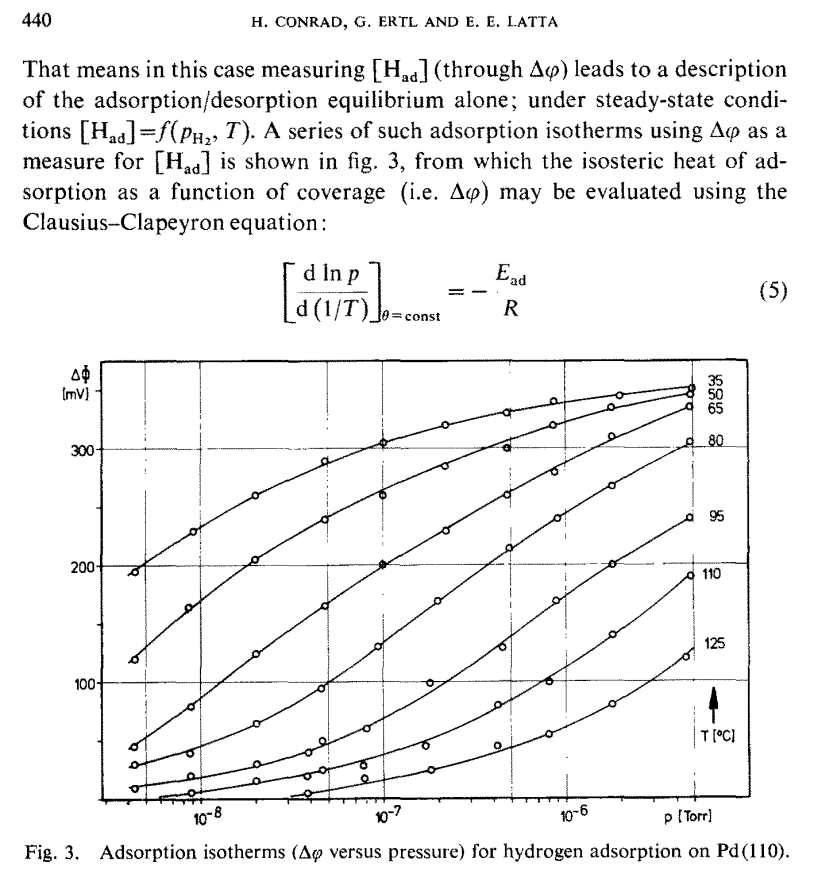
\includegraphics{conrad1974_fig3.png}
\caption{conrad1974\_fig3.png}
\end{figure}

    \begin{figure}
\centering
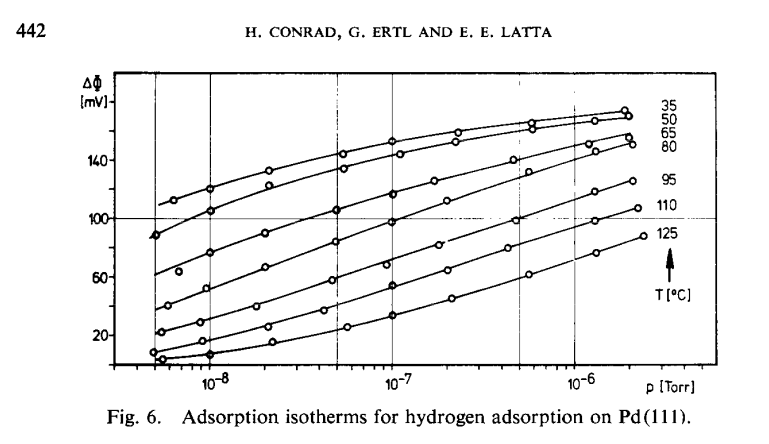
\includegraphics{conrad1974_fig6.png}
\caption{conrad1974\_fig6.png}
\end{figure}

    Из сравнения этих изотерм видно что при одном и том же давлении водорода
в газовой фазе и для одной и той же температуры поверхностная
концентрация водорода для более рыхлой поверхности \(Pd(110)/H\) имеет
более высокие значения чем оные для более гладкой поверхности
\(Pd(111)/H\).

    При одной и той же температуре и давлении газообразного молекулярного
водорода степень насыщения адсорбированным водородом более рыхлой
поверхности Pd(110) в целом выше оной для более гладкой поверхности
Pd(111).

Правда найденные изотермы сложны тем что в них по вертикальной оси
приводятся данные \(\Delta \varphi\) которые пропорциональны степени
поверхностного насыщения \(\Theta\), но перевод вертикально оси этих в
изотерм в \(\Theta\) не выполнен.

Поэтому на их основании можно сделать следующий предварительный расчёт

Предполагая, что одно и то же значение \(\Delta \varphi = 165 mV\) для
обоих поверхностей \(Pd(110)/H\) и \(Pd(111)/H\) при одной и той же
температуре \(T = 35 ^{\circ} C\) соответствует одной и той же (пока что
невыясненной) степени насыщения поверхности водородом, найдем теперь
разницу равновесных давлений газообразного водорода при этой температуре
при данной степени насыщения.

Для поверхности \(Pd(110)/H\) равновесное давление

\(p_{Pd(110)} = 2 \cdot 10^{-9} Torr = 2.66 \cdot 10^{-7} Pa\)

\(\sqrt{p_{Pd(110)}} = 0.0005157519 Pa^{-1/2}\)

Для поверхности \(Pd(111)/H\) равновесное давление

\(p_{Pd(111)} = 10^{-6} Torr = 1.33 \cdot 10^{-4} Pa\)

\(\sqrt{p_{Pd(111)}} = 0.01153256 Pa^{-1/2}\)

    Далее в работе

\begin{enumerate}
\def\labelenumi{\arabic{enumi}.}
\setcounter{enumi}{34}
\tightlist
\item
  Nishimura C., Komaki M., Amano M. Hydrogen permeation characteris-
  tics of vanadium-nickel alloys // Mater. Trans. 1991. Vol. 32(5). P.
  501--507 {[}https://doi.org/10.2320/matertrans1989.32.501{]}.
\end{enumerate}

приводится формула для потока через мембрану

\(J = \Phi \left(P_u^{1/2} - P_d^{1/2} \right) \big / L\)

\(J =\) steady state hydrogen flux
\(\left(mol \,\,\, of \,\,\, H_2 \big/ \left(m^2 \cdot s\right)\right)\)

\(\Phi =\) hydrogen permeability
\(\left(mol \,\,\, of \,\, H_2 \big/ \left(m \cdot s \cdot Pa^{1/2}\right)\right)\)

\(P_u, P_d\) hydrogen pressures at the upstream side and the downstream
side \(Pa\)

В этой же работе приводится график

    \begin{figure}
\centering
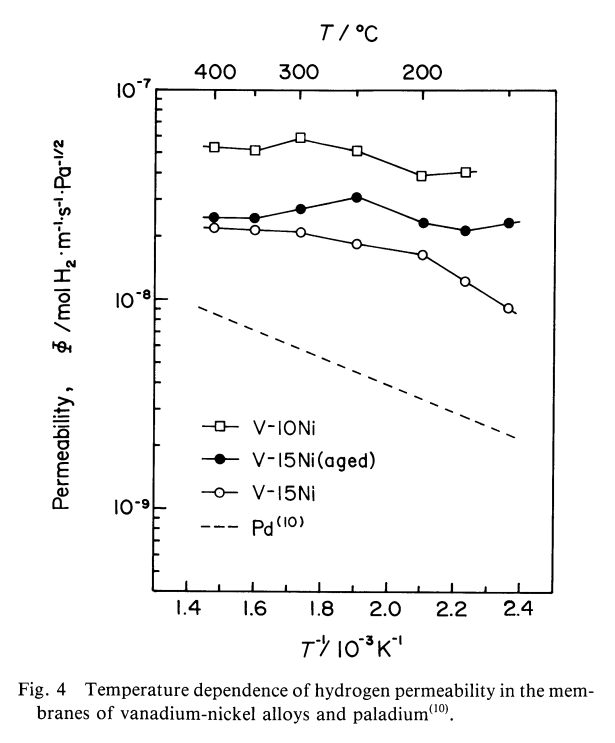
\includegraphics{nishimura1991_fig4.png}
\caption{nishimura1991\_fig4.png}
\end{figure}

    Из этого графика для температуры \(T = 35 ^{\circ} C = 308 K\) для
палладиевой мембраны

\(\Phi = 6 \cdot 10^{-9} mol \,\, H_2 \cdot m^{-1} \cdot s^{-1} \cdot Pa^{-1/2}\)

для мембраны из сплава ванадия с 10 \% никеля

\(\Phi = 6 \cdot 10^{-8} mol \,\, H_2 \cdot m^{-1} \cdot s^{-1} \cdot Pa^{-1/2}\)

исходя из этих данных можно вычислить стационарный поток через при
указанной разности давлений

\(J = \Phi \left(P_u^{1/2} - P_d^{1/2} \right) \big / L\)

    \begin{tcolorbox}[breakable, size=fbox, boxrule=1pt, pad at break*=1mm,colback=cellbackground, colframe=cellborder]
\prompt{In}{incolor}{68}{\boxspacing}
\begin{Verbatim}[commandchars=\\\{\}]
\PY{n}{Phi\PYZus{}Pd}     \PY{o}{=} \PY{l+m+mi}{6} \PY{o}{*} \PY{l+m+mi}{10}\PY{o}{\PYZca{}}\PY{p}{(}\PY{o}{\PYZhy{}}\PY{l+m+mi}{9}\PY{p}{)}    \PY{c+c1}{\PYZsh{} mol \PYZbs{},\PYZbs{}, H\PYZus{}2 \PYZbs{}cdot m\PYZca{}\PYZob{}\PYZhy{}1\PYZcb{} \PYZbs{}cdot s\PYZca{}\PYZob{}\PYZhy{}1\PYZcb{} \PYZbs{}cdot Pa\PYZca{}\PYZob{}\PYZhy{}1/2\PYZcb{}\PYZdl{}}
\PY{n}{Phi\PYZus{}V\PYZus{}10Ni} \PY{o}{=} \PY{l+m+mi}{6} \PY{o}{*} \PY{l+m+mi}{10}\PY{o}{\PYZca{}}\PY{p}{(}\PY{o}{\PYZhy{}}\PY{l+m+mi}{8}\PY{p}{)}    \PY{c+c1}{\PYZsh{} mol \PYZbs{},\PYZbs{}, H\PYZus{}2 \PYZbs{}cdot m\PYZca{}\PYZob{}\PYZhy{}1\PYZcb{} \PYZbs{}cdot s\PYZca{}\PYZob{}\PYZhy{}1\PYZcb{} \PYZbs{}cdot Pa\PYZca{}\PYZob{}\PYZhy{}1/2\PYZcb{}\PYZdl{}}
\PY{n}{p\PYZus{}Pd\PYZus{}111}   \PY{o}{=} \PY{l+m+mf}{1.33} \PY{o}{*} \PY{l+m+mi}{10}\PY{o}{\PYZca{}}\PY{p}{(}\PY{o}{\PYZhy{}}\PY{l+m+mi}{4}\PY{p}{)} \PY{c+c1}{\PYZsh{} Pa}
\PY{n}{p\PYZus{}Pd\PYZus{}110}   \PY{o}{=} \PY{l+m+mf}{2.66} \PY{o}{*} \PY{l+m+mi}{10}\PY{o}{\PYZca{}}\PY{p}{(}\PY{o}{\PYZhy{}}\PY{l+m+mi}{7}\PY{p}{)} \PY{c+c1}{\PYZsh{} Pa}
\PY{n}{L}          \PY{o}{=} \PY{l+m+mi}{10}\PY{o}{*}\PY{l+m+mi}{10}\PY{o}{\PYZca{}}\PY{p}{(}\PY{o}{\PYZhy{}}\PY{l+m+mi}{6}\PY{p}{)}     \PY{c+c1}{\PYZsh{} m \PYZhy{} толщина мембраны 10 микрон}
\PY{n}{R}          \PY{o}{=} \PY{l+m+mf}{8.31446262}     \PY{c+c1}{\PYZsh{} м\PYZca{}2 кг с\PYZca{}\PYZhy{}2 К\PYZca{}\PYZhy{}1 Моль\PYZca{}\PYZhy{}1}
\PY{n}{T}          \PY{o}{=} \PY{l+m+mi}{308}            \PY{c+c1}{\PYZsh{} K}
\end{Verbatim}
\end{tcolorbox}

    \(J =\) steady state hydrogen flux
\(\left(mol \,\,\, of \,\,\, H_2 \big/ \left(m^2 \cdot s\right)\right)\)

    \begin{tcolorbox}[breakable, size=fbox, boxrule=1pt, pad at break*=1mm,colback=cellbackground, colframe=cellborder]
\prompt{In}{incolor}{69}{\boxspacing}
\begin{Verbatim}[commandchars=\\\{\}]
\PY{n}{J\PYZus{}Pd} \PY{o}{=} \PY{n}{Phi\PYZus{}Pd} \PY{o}{*} \PY{p}{(}\PY{n}{sqrt}\PY{p}{(}\PY{n}{p\PYZus{}Pd\PYZus{}111}\PY{p}{)} \PY{o}{\PYZhy{}} \PY{n}{sqrt}\PY{p}{(}\PY{n}{p\PYZus{}Pd\PYZus{}110}\PY{p}{)}\PY{p}{)}\PY{o}{/}\PY{n}{L}
\PY{n}{J\PYZus{}Pd}
\end{Verbatim}
\end{tcolorbox}

            \begin{tcolorbox}[breakable, size=fbox, boxrule=.5pt, pad at break*=1mm, opacityfill=0]
\prompt{Out}{outcolor}{69}{\boxspacing}
\begin{Verbatim}[commandchars=\\\{\}]
6.61008642980501e-6
\end{Verbatim}
\end{tcolorbox}
        
    \begin{tcolorbox}[breakable, size=fbox, boxrule=1pt, pad at break*=1mm,colback=cellbackground, colframe=cellborder]
\prompt{In}{incolor}{70}{\boxspacing}
\begin{Verbatim}[commandchars=\\\{\}]
\PY{n}{J\PYZus{}V\PYZus{}10Ni} \PY{o}{=} \PY{n}{Phi\PYZus{}V\PYZus{}10Ni} \PY{o}{*} \PY{p}{(}\PY{n}{sqrt}\PY{p}{(}\PY{n}{p\PYZus{}Pd\PYZus{}111}\PY{p}{)} \PY{o}{\PYZhy{}} \PY{n}{sqrt}\PY{p}{(}\PY{n}{p\PYZus{}Pd\PYZus{}110}\PY{p}{)}\PY{p}{)}\PY{o}{/}\PY{n}{L}
\PY{n}{J\PYZus{}V\PYZus{}10Ni}
\end{Verbatim}
\end{tcolorbox}

            \begin{tcolorbox}[breakable, size=fbox, boxrule=.5pt, pad at break*=1mm, opacityfill=0]
\prompt{Out}{outcolor}{70}{\boxspacing}
\begin{Verbatim}[commandchars=\\\{\}]
0.0000661008642980501
\end{Verbatim}
\end{tcolorbox}
        
    Допустим что установление потока в 4 раза уменьшит величину P\_Pd\_111 и
в столько же раз увеличит величину p\_Pd\_110 тогда

    \begin{tcolorbox}[breakable, size=fbox, boxrule=1pt, pad at break*=1mm,colback=cellbackground, colframe=cellborder]
\prompt{In}{incolor}{71}{\boxspacing}
\begin{Verbatim}[commandchars=\\\{\}]
\PY{n}{k} \PY{o}{=} \PY{l+m+mi}{4}

\PY{n}{p\PYZus{}Pd\PYZus{}111\PYZus{}k} \PY{o}{=} \PY{n}{p\PYZus{}Pd\PYZus{}111}\PY{o}{/}\PY{n}{k}
\PY{n}{p\PYZus{}Pd\PYZus{}110\PYZus{}k} \PY{o}{=} \PY{n}{p\PYZus{}Pd\PYZus{}110}\PY{o}{*}\PY{n}{k}
\end{Verbatim}
\end{tcolorbox}

    \begin{tcolorbox}[breakable, size=fbox, boxrule=1pt, pad at break*=1mm,colback=cellbackground, colframe=cellborder]
\prompt{In}{incolor}{72}{\boxspacing}
\begin{Verbatim}[commandchars=\\\{\}]
\PY{n}{J} \PY{o}{=} \PY{n}{Phi\PYZus{}V\PYZus{}10Ni} \PY{o}{*} \PY{p}{(}\PY{n}{sqrt}\PY{p}{(}\PY{n}{p\PYZus{}Pd\PYZus{}111\PYZus{}k}\PY{p}{)} \PY{o}{\PYZhy{}} \PY{n}{sqrt}\PY{p}{(}\PY{n}{p\PYZus{}Pd\PYZus{}110\PYZus{}k}\PY{p}{)}\PY{p}{)}\PY{o}{/}\PY{n}{L}
\PY{n}{J}
\end{Verbatim}
\end{tcolorbox}

            \begin{tcolorbox}[breakable, size=fbox, boxrule=.5pt, pad at break*=1mm, opacityfill=0]
\prompt{Out}{outcolor}{72}{\boxspacing}
\begin{Verbatim}[commandchars=\\\{\}]
0.0000284086652440631
\end{Verbatim}
\end{tcolorbox}
        
    Скорость потока в газовой фазе в метрах в секунду

\(v = \frac{J}{c} = J \frac{R T}{p}\)

    \begin{tcolorbox}[breakable, size=fbox, boxrule=1pt, pad at break*=1mm,colback=cellbackground, colframe=cellborder]
\prompt{In}{incolor}{73}{\boxspacing}
\begin{Verbatim}[commandchars=\\\{\}]
\PY{n}{v\PYZus{}Pd\PYZus{}111} \PY{o}{=} \PY{n}{J} \PY{o}{*} \PY{n}{R} \PY{o}{*} \PY{n}{T} \PY{o}{/} \PY{p}{(}\PY{n}{p\PYZus{}Pd\PYZus{}111\PYZus{}k}\PY{p}{)}
\PY{n}{v\PYZus{}Pd\PYZus{}111}
\end{Verbatim}
\end{tcolorbox}

            \begin{tcolorbox}[breakable, size=fbox, boxrule=.5pt, pad at break*=1mm, opacityfill=0]
\prompt{Out}{outcolor}{73}{\boxspacing}
\begin{Verbatim}[commandchars=\\\{\}]
2187.98369500161
\end{Verbatim}
\end{tcolorbox}
        
    \begin{tcolorbox}[breakable, size=fbox, boxrule=1pt, pad at break*=1mm,colback=cellbackground, colframe=cellborder]
\prompt{In}{incolor}{74}{\boxspacing}
\begin{Verbatim}[commandchars=\\\{\}]
\PY{n}{v\PYZus{}Pd\PYZus{}110} \PY{o}{=} \PY{n}{J} \PY{o}{*} \PY{n}{R} \PY{o}{*} \PY{n}{T} \PY{o}{/} \PY{p}{(}\PY{n}{p\PYZus{}Pd\PYZus{}110\PYZus{}k}\PY{p}{)}
\PY{n}{v\PYZus{}Pd\PYZus{}110}
\end{Verbatim}
\end{tcolorbox}

            \begin{tcolorbox}[breakable, size=fbox, boxrule=.5pt, pad at break*=1mm, opacityfill=0]
\prompt{Out}{outcolor}{74}{\boxspacing}
\begin{Verbatim}[commandchars=\\\{\}]
68374.4904688004
\end{Verbatim}
\end{tcolorbox}
        
    Оценка мощности по формуле аналогичной оной в работе
"жидкокристаллический осмос"

\(w = \eta \cdot p \cdot V_{ос}\,\,\,\frac{Вт}{м^2}\)

    \begin{tcolorbox}[breakable, size=fbox, boxrule=1pt, pad at break*=1mm,colback=cellbackground, colframe=cellborder]
\prompt{In}{incolor}{75}{\boxspacing}
\begin{Verbatim}[commandchars=\\\{\}]
\PY{n}{eta} \PY{o}{=} \PY{l+m+mf}{0.5}

\PY{n}{v\PYZus{}osmos} \PY{o}{=} \PY{p}{(}\PY{n}{v\PYZus{}Pd\PYZus{}111} \PY{o}{+} \PY{n}{v\PYZus{}Pd\PYZus{}110}\PY{p}{)} \PY{o}{/} \PY{l+m+mi}{2}
\PY{n}{p\PYZus{}osmos} \PY{o}{=} \PY{p}{(}\PY{n}{p\PYZus{}Pd\PYZus{}111\PYZus{}k} \PY{o}{\PYZhy{}} \PY{n}{p\PYZus{}Pd\PYZus{}110\PYZus{}k}\PY{p}{)}

\PY{n}{w} \PY{o}{=} \PY{l+m+mf}{0.5} \PY{o}{*} \PY{n}{p\PYZus{}osmos} \PY{o}{*} \PY{n}{v\PYZus{}osmos}
\PY{n}{w} 
\end{Verbatim}
\end{tcolorbox}

            \begin{tcolorbox}[breakable, size=fbox, boxrule=.5pt, pad at break*=1mm, opacityfill=0]
\prompt{Out}{outcolor}{75}{\boxspacing}
\begin{Verbatim}[commandchars=\\\{\}]
0.567780948359033
\end{Verbatim}
\end{tcolorbox}
        
    итак, \(w \approx 567\,мВт/м^2\).

Если взять мембрану из ванадия толщиной 10 микрон но покрытой с обеих
сторон \(Pd(110)\) и \(Pd(111)\) и площадью 10 на 10 сантиметров, то
мощность снимаемая с одной такой мембраны будет порядка

    \begin{tcolorbox}[breakable, size=fbox, boxrule=1pt, pad at break*=1mm,colback=cellbackground, colframe=cellborder]
\prompt{In}{incolor}{77}{\boxspacing}
\begin{Verbatim}[commandchars=\\\{\}]
\PY{n}{w} \PY{o}{*} \PY{l+m+mi}{10}\PY{o}{\PYZca{}}\PY{p}{(}\PY{o}{\PYZhy{}}\PY{l+m+mi}{2}\PY{p}{)} \PY{o}{*} \PY{l+m+mi}{10}\PY{o}{\PYZca{}}\PY{l+m+mi}{3}
\end{Verbatim}
\end{tcolorbox}

            \begin{tcolorbox}[breakable, size=fbox, boxrule=.5pt, pad at break*=1mm, opacityfill=0]
\prompt{Out}{outcolor}{77}{\boxspacing}
\begin{Verbatim}[commandchars=\\\{\}]
5.67780948359033
\end{Verbatim}
\end{tcolorbox}
        
    \(5.67\) мВт. Но если сделать стопку таких мембран общей высотой 10
сантиметров, то при расстоянии между мембранами 10 микрон можно иметь в
такой стопке 50 тысяч мембран. Тогда суммарная мощность такой мембранной
системы может достигать \(283\) Ватт.

    \begin{tcolorbox}[breakable, size=fbox, boxrule=1pt, pad at break*=1mm,colback=cellbackground, colframe=cellborder]
\prompt{In}{incolor}{78}{\boxspacing}
\begin{Verbatim}[commandchars=\\\{\}]
\PY{n}{w}\PY{o}{*}\PY{l+m+mi}{5}\PY{o}{*}\PY{l+m+mi}{10}\PY{o}{\PYZca{}}\PY{l+m+mi}{4}\PY{o}{/}\PY{l+m+mi}{100}
\end{Verbatim}
\end{tcolorbox}

            \begin{tcolorbox}[breakable, size=fbox, boxrule=.5pt, pad at break*=1mm, opacityfill=0]
\prompt{Out}{outcolor}{78}{\boxspacing}
\begin{Verbatim}[commandchars=\\\{\}]
283.890474179517
\end{Verbatim}
\end{tcolorbox}
        
    Таким образом оценка ожидаемой мощности водород биметаллического
кольцара в 50 раз выше оценки мощности жидкокристаллического осмоса

    Но технологически довольно сложно все получается - нужно делать мембрану
толщиной 10 микрон симметричная основа которой - сплав ванадия + 10\%
никеля, покрытия - микронные слои палладия с 2-х сторон, необходимая
асимметрия - благодаря различному значению hkl поверхности
моноклисталлической поверхности слоя.

Насколько это реально технологически?

И чтобы получить из 1 литра мембранной системы 283 ватт, нужно 50 тысяч
таких мембран толщиной 10 микрон и между ними газовый промежуток 10
микрон

Расчёт произведен для весьма низких давлений газообразного водорода
порядка 10\^{}-6 .... 10\^{}-9 мм ртутного столба.

Как изменится оценка ожидаемой мощности при увеличении давления
водорода, пока не ясно потому что мне пока не попались изотермы
диссоциации для более высоких давлений - там непонятно что будет
происходить с молекулярным водородом для комнатных температур - вот у
Чапека со смесью атомарого и молекулярного водорода при высоких
температурах например эффект уменьшается при увеличении давления

    \begin{figure}
\centering
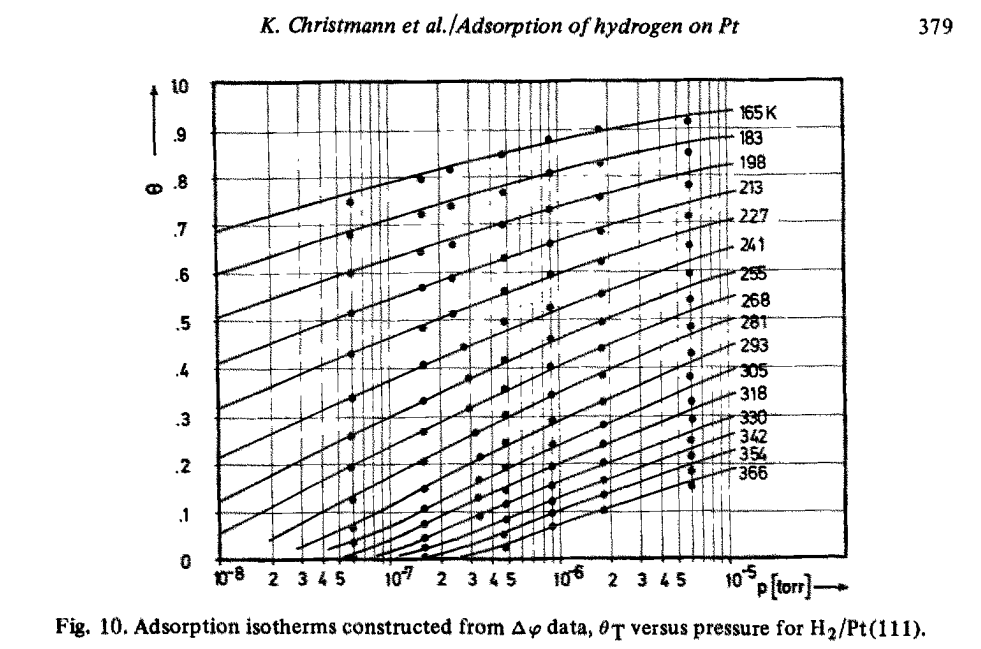
\includegraphics{christmann1976_fig10.png}
\caption{christmann1976\_fig10.png}
\end{figure}

    Правда данная методика расчёта не учитывает влияние возможного обратного
градиента давления (или обратного натяжения), которое согласно
классическим термодинамическим представлениям должно бы возникнуть в
области спая этих двух монокристаллов с разными hkl. И это
противодавление, согласно термодинамическим представлениям должно
препятствовать возникновению вышеуказанной осмотический силы кольцара.

Действительно, представим себе что мы разлепили два спаянных
монокристалла и развели их на известное расстояние, не изменяя степени
насыщения металла водородом. Тогда внешняя разность давлений полностью
будет компенсироваться обратно направленной внутренней разностью
давлений.

Для того чтобы понять что произойдёт, если мы, не меняя степени
насыщения металла водородом, обратно слепим два монокристалла в спай,
нужно себе уяснить следующий вопрос: а какова физическая причина того,
что для для одного и того же металла, при одной и той же температуре
металла, насыщенного водородом, для одной и той же степени насыщения
металла водородом, но для разных поверхностей среза hkl монокристалла
получаются разные равновесные давления водорода в газовой фазе.

Выше я уже указывал на одну из, на мой взгляд, важных физических причин
этого: кинетика процесса десорбции определяется в том числе и таким
фактором как дифракция волн де Бройля молекул водорода на
кристаллической решётке, которую эти молекулы пытаются покинуть. А
параметры дифракции, как известно определяются шагом дифракционной
решётки, который разный для разных hkl.

Так вот, когда мы слепляем обратно в спай два монокристалла, условия
дифракции нарушаются из-за чисто геометрических причин: зазор между
поверхностями исчезает. И следовательно исчезает (полностью или не
полностью пока не понятно) внутренняя разница равновесных давлений,
которая теперь если и пытается компенсировать возникновение осмотической
силы кольцара, но полностью ее скомпенсировать она не в состоянии.

    

    \section{Метод оценки на основании данных о кинетике
адсорбции}\label{ux43cux435ux442ux43eux434-ux43eux446ux435ux43dux43aux438-ux43dux430-ux43eux441ux43dux43eux432ux430ux43dux438ux438-ux434ux430ux43dux43dux44bux445-ux43e-ux43aux438ux43dux435ux442ux438ux43aux435-ux430ux434ux441ux43eux440ux431ux446ux438ux438}

    Что важно учесть - поверхности могут отличаться первым или вторым
порядком кинетики процессов адсорбции или десорбции.

    Для поверхностей характеризующихся кинетикой десорбции второго порядка
можно записать следующее выражение для концентрации молекул водорода в
газовой фазе через предэкспоненциальный множитель кинетики десорбции
(Frequency factor, \(\nu_{2} (cm^{2} s^{-1} H-atom^{-1})\)), коэффициент
прилипания \(s_0\), активационный барьер процесса десорбции
\(\Delta E^{*}_{d}\left(\Theta\right)\), поверхностную концентрацию
адсорбированных атомов водорода \(n_{ad}\) и среднюю скорость молекул
водорода в газовой фазе \({\overset{-}c}\)

    \(s_0\overset{-}c n_g = \nu_2 \left(\Theta\right) \, exp \left(-\frac{\Delta E^{*}_{d} \left(\Theta\right)}{kT} \right) n_{ad}^2\)

    \(n_g = \frac{\nu_2 \left(\Theta\right)}{s_0} \, exp \left(-\frac{\Delta E^{*}_{d} \left(\Theta\right)}{kT} \right) \frac{n_{ad}^2}{\overset{-}c}\)

    \[\begin{array}{rrrr}
Metal      & \nu_{2}                &    s_0            & \Delta E^{*}_{d} \\
(hkl)      & \frac{cm^{2}}{s \, at} &                   &       kJ/mol     \\
Ni(100)    & 3 \times 10^{0}        & 0.06-0.1 (120 K)  & ...              \\
           & 2.5 \times 10^{-1}     &                   & ...              \\
           & 8 \times 10^{-2}       &                   & ...              \\
           & 5 \times 10^{-2}       &                   & ...              \\
Ni(111)    & 2 \times 10^{-1}       & 0.05 (120 K)      & ...              \\
           & 2.3 \times 10^{-2}     & 0.1  (140 K)      & ...              \\
Pd(100)    & 1 \times 10^{-2}       & 0.5  (120 K)      & ...              \\
Pd(110)    & 8 \times 10^{-2}       & 0.7  (120 K)      & ...              \\
\end{array}\]

    Для поверхностей характеризующихся кинетикой десорбции первого порядка
можно записать следующее выражение для концентрации молекул водорода в
газовой фазе через предэкспоненциальный множитель кинетики десорбции
(Frequency factor, \(\nu_{1} (s^{-1})\)), коэффициент прилипания
\(s_0\), активационный барьер процесса десорбции
\(\Delta E^{*}_{d}\left(\Theta\right)\), поверхностную концентрацию
адсорбированных атомов водорода \(n_{ad}\) и среднюю скорость молекул
водорода в газовой фазе \({\overset{-}c}\)

    \(s_0\overset{-}c n_g = \nu_1 \, exp \left(-\frac{\Delta E^{*}_{d}}{kT} \right) \frac{n_{ad}}{2}\)

    \(n_g = \frac{\nu_1}{s_0} \, exp \left(-\frac{\Delta E^{*}_{d}}{kT} \right) \frac{n_{ad}}{2\overset{-}c}\)

    сообщается о кинетике десорбции первого порядка, когда заселяются
дополнительные низкоэнергетические состояния связывания. Примерами
являются состояние \(\beta_1\) для \(H\) на \(Ni(110)\) {[}230,231{]},
состояния \(\alpha_1\) и \(\alpha_2\) для Rh(110) {[}70{]}, состояния
\(\alpha_1\) и \(\alpha_2\) для \(H\) на \(Pd(110)\) {[}68{]}.

предполагается, что либо силы латерального взаимодействия, зависящие от
покрытия, либо структурные фазовые изменения в адсорбированном слое во
время температурной программы ответственны за «псевдопервопорядковую»
кинетику. Действительно, для системы \(Rh(110)/H\) {[}70{]} тщательное
изучение спектров TPD выявило небольшие сдвиги пиков, указывающие на
возможную незначительную кинетику десорбции дробного порядка. Это может
быть вызвано, например, преимущественной десорбцией с концов линейных
цепочек H, которые образуются вдоль впадин этой (110) поверхности. Кроме
того, в случае \(Pd(110)/H\) и \(Ni(110)/H\) адсорбции явно сопутствуют
явления реконструкции поверхности и/или заселения приповерхностных
участков {[}275{]}, которые также изменяют кинетику десорбции.

    \[\begin{array}{rrrr}
Metal      & \nu_{1}                  &    s_0        & \Delta E^{*}_{d} \\
(hkl)      & \left(\frac{1}{s}\right) &               &       kJ/mol     \\
Ni(110)    &                          & 0.96 (120 K)  & ...              \\
           &                          & 0.4  (300 K)  & ...              \\
\end{array}\]

    \section{Физико-химическое происхождение сверхпроницаемости -
крупномасштабное влияние химии поверхности на проницаемость и поглощение
«горячего» водорода в
металлах}\label{ux444ux438ux437ux438ux43aux43e-ux445ux438ux43cux438ux447ux435ux441ux43aux43eux435-ux43fux440ux43eux438ux441ux445ux43eux436ux434ux435ux43dux438ux435-ux441ux432ux435ux440ux445ux43fux440ux43eux43dux438ux446ux430ux435ux43cux43eux441ux442ux438---ux43aux440ux443ux43fux43dux43eux43cux430ux441ux448ux442ux430ux431ux43dux43eux435-ux432ux43bux438ux44fux43dux438ux435-ux445ux438ux43cux438ux438-ux43fux43eux432ux435ux440ux445ux43dux43eux441ux442ux438-ux43dux430-ux43fux440ux43eux43dux438ux446ux430ux435ux43cux43eux441ux442ux44c-ux438-ux43fux43eux433ux43bux43eux449ux435ux43dux438ux435-ux433ux43eux440ux44fux447ux435ux433ux43e-ux432ux43eux434ux43eux440ux43eux434ux430-ux432-ux43cux435ux442ux430ux43bux43bux430ux445}

    Livshits A. I., Notkin M. E., Samartsev A. A. Physico-Chemical Origin of
Superpermeability-Large-Scale Effects of Surface Chemistry on «Hot»
Hydrogen Permeation and Absorption in Metals // J. Nucl. Mater. 1990.
Vol. 170, N 1. P. 79--94
{[}https://doi.org/10.1016/0022-3115(90)90329-L{]}.

    \begin{figure}
\centering
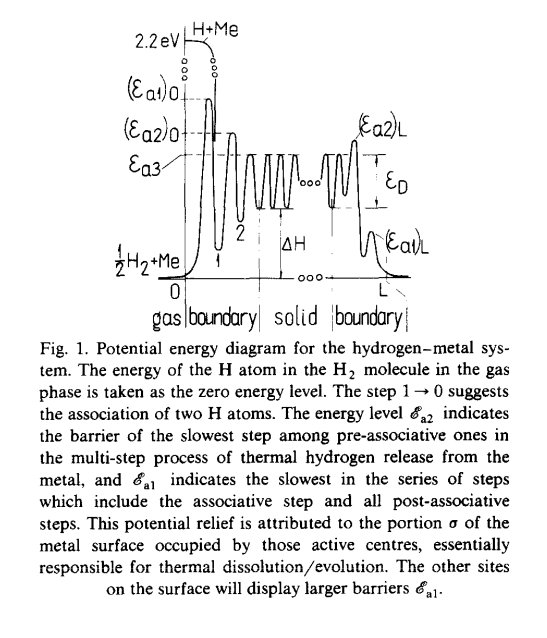
\includegraphics{livshits1990_Fig01.png}
\caption{livshits1990\_Fig01.png}
\end{figure}

    2.1. Kinetics of dissolution and evolution

Hydrogen dissolution and evolution by metals should be considered as
multi-step processes. Now, as it follows from a simple phenomenological
treatment, super-permeability will be possible only when the rate of
thermal evolution is controlled either by the associative step itself or
by any post-associative step {[}4-6{]}. In this case, the process of
thermal evolution is second order in subsurface concentration, \(c\), of
dissolved hydrogen, and the probability of thermal dissolution of a
hydrogen gas molecule at one impact on a metal surface equals the
probability of dissociative binding of the molecule, \(\alpha\).
Correspondingly, the rates of thermal dissolution, \(j_a\), and
evolution, \(j_r\), are given (at a condition that surface coverage by
hydrogen is far from saturation) by

\begin{equation}
\begin{array}{ll}
j_{a0} = \alpha_0 Z p, & j_{r0} = k_{r0} c_0^2 , \\
j_{aL} = \alpha_L Z p, & j_{rL} = k_{rL} c_L^2 , \\
\end{array}
\end{equation}

    where \(p\) is hydrogen pressure, \(Z\) is the kinetic theory
coefficient (\(Z = (2 \pi m k T)^{-1/2}\), where \(m\) is the mass of
the gas molecule, and \(k\) is Boltzmann's constant;
\(Z \approx 1.2 \times 10^{19} H_2 \big /(cm^2 \, s \, Pa)\) at 20
\(^{\circ}C\)), \(k_{rO}\) and \(k_{rL}\) are the rate constants for
evolution, with indices \(0\) and \(L\) referring to the inlet
(upstream) and outlet (downstream) surfaces, respectively. The
probabilities \(\alpha\) may be presented as

\begin{equation}
\begin{array}{l}
\alpha_0 = \alpha_{0}^{*}  \sigma_0 \, exp\left[ -2 \left(E_{a1}\right)_0 \right / RT], \\
\alpha_L = \alpha_{L}^{*} \sigma_L \, exp\left[ -2 \left(E_{a1}\right)_L\right / RT], \\
\end{array}
\end{equation}

    the barriers \(E_{a1}\) are shown in fig. 1. The quantities
\(\alpha_{0}^{*}\) and \(\alpha_{L}^{*}\) are pre-exponentials in the
order of \(0.1-1\) while \(\sigma_0\), and \(\sigma_L\) are fractions of
the surfaces occupied by the centres active in the dissolution-evolution
kinetics considered \# (for a homogeneous surface \(\sigma = 1\)).

The remaining part \(1 - \sigma\) of the surface has a larger \(E_{a1}\)
barrier.

    From balancing the fluxes, it follows that \(k_r = \alpha Z / S^2\),
where \(S\) is the equilibrium (Sieverts') constant for dilute solution
of hydrogen in the metal contacting gas phase hydrogen:

\(S=S* exp(-\Delta H/RT);(3)\)

\(\Delta H\) is the enthalpy of solution (see fig. 1, and the table of
notation in the Appendix).

    \section{2.4. Non-symmetric membranes}\label{non-symmetric-membranes}

Seen from eqs. (4) is that a non-symmetric membrane
(\(\alpha_0 \neq \alpha_L\)) may exhibit conspicuous differences in the
permeability to ``hot'' gas for the two opposite directions of gas flow
(i.e. for \(\alpha_0\) and \(\alpha_L\) interchanged). This trait is
peculiar to non-equilibrium conditions, whereas the permeability to the
molecular hydrogen gas is the same in either direction for both the
extremes given by eqs. (10 a) and (10 b). We have to dwell on the latter
point, since arguing about it resumes intermittently in the literature
{[}34,35{]}.

{[}34{]} N.I. Ionov. Sov. Phys. - Solid State 27 (1985) 1527.

{[}35{]} W.A. Swansiger and D.R. Folk, Rev. Sci. Instr. 58 (1987) 1266.

    \section{2.4. Несимметричные
мембраны}\label{ux43dux435ux441ux438ux43cux43cux435ux442ux440ux438ux447ux43dux44bux435-ux43cux435ux43cux431ux440ux430ux43dux44b}

Из уравнений (4) следует, что несимметричная мембрана
(\(\alpha_0 \neq \alpha_L\)) может демонстрировать заметные различия в
проницаемости для «горячего» газа для двух противоположных направлений
потока газа (т.е. для \(\alpha_0\) и \(\alpha_L\), чередующихся между
собой). Эта особенность свойственна неравновесным условиям, тогда как
проницаемость для молекулярного водородного газа одинакова в любом
направлении для обоих экстремумов, задаваемых уравнениями (10a) и (10b).
На последнем моменте мы вынуждены остановиться, поскольку споры о нем
периодически возобновляются в литературе {[}34,35{]}.

    Permeation differences in the different directions are not entirely
prohibited for a non-symmetric membrane separating an equilibrium gas at
some specific pressure from the vacuum, or from the gas at another
pressure, if more complicated mechanisms of hydrogen-metal interaction
are involved than those assumed to obtain eqs. (4) and (10) *. But any
kinetic formalism being contemplated to account for an asymmetric
permeation should meet one requirement stipulated by the principles of
thermodynamics: no regular gas flow may exist under isothermic
conditions, if hydrogen pressures are equal on the both sides of a
membrane.

    Для несимметричной мембраны, отделяющей равновесный газ при некотором
определенном давлении от вакуума или от газа при другом давлении, не
исключены различия в проницаемости в разных направлениях, если
задействованы более сложные механизмы взаимодействия водорода с
металлом, чем те, которые предполагаются для получения уравнений (4) и
(10)*. Но любой кинетический формализм, рассматриваемый для учета
асимметричной проницаемости, должен удовлетворять одному требованию,
обусловленному принципами термодинамики: регулярный поток газа не может
существовать в изотермических условиях, если давления водорода по обе
стороны мембраны равны.

    Отсюда я делаю вывод, что авторы (Livshits A. I., Notkin M. E.,
Samartsev A. A.) придерживаются, на мой взгляд, ошибочного мнения о
термодинамическом, а не о статистическом характере второго начала
термодинамики. Но ладно, все равно интересно что пишут авторы о
несимметричных мембранах

    This requirement appears to be disregarded by alleging that the
deposition of palladium overlayers only on the upstream surface of the
originally symmetric membranes of stainless steel {[}37{]} or niobium
{[}38{]} should bring about a sharp rise of their permeability to
molecular hydrogen owed simply to the easier hydrogen dissociation and
dissolution characteristic of palladium. A similar argument {[}34{]}
will infer a non-zero gas flow, if applied to the situation of equal
pressures at either side of the asymmetric membrane. Again, the
possibility of easier dissolution on the upstream side is included in
eq. (10a). The quantities \(\alpha_0\) and \(\alpha_L\), pertaining to
the two membrane sides, are equipollent there, and a two-fold permeation
increase maximally may result from enhancing the rate of dissolution at
only one side of a symmetric membrane.

    Это требование, по-видимому, игнорируется, если утверждать, что
нанесение палладиевых слоев только на верхнюю поверхность первоначально
симметричных мембран из нержавеющей стали {[}37{]} или ниобия {[}38{]}
должно привести к резкому увеличению их проницаемости для молекулярного
водорода просто в силу более легкой диссоциации и растворения водорода,
характерных для палладия. Аналогичный аргумент {[}34{]} приведет к
ненулевому потоку газа, если применить его к ситуации равных давлений по
обе стороны асимметричной мембраны. Опять же, возможность более легкого
растворения со стороны восходящего потока включена в уравнение (10a).
Величины \(\alpha_0\) и \(\alpha_L\), относящиеся к двум сторонам
мембраны, здесь эквиполентны, и максимальное двукратное увеличение
проницаемости может быть достигнуто за счет увеличения скорости
растворения только на одной стороне симметричной мембраны.

    A notice should be given to one possible source of mistake in assessing
the data of experiments with molecular hydrogen. In a real experimental
set-up, the temperature of the gas acting on a metal sample may differ
from the metal temperature. The sample can be heated, while the gas may
retain essentially the temperature of the walls of vacuum chamber. The
effects may develop in these circumstances, characteristics of
non-equilibrium conditions.

For example, the probability of absorption of a hydrogen molecule at the
surface of copper is known to depend on the molecule kinetic energy
{[}39,40{]}, whereas clean palladium absorbs the impinging molecules
with a probability of the order of unity, irrespective of their velocity
{[}20,40{]}. A palladium membrane having a very thin copper coating on
one surface may, therefore, display an asymmetric permeability to a gas
that is ``colder'' than the membrane. The permeation will be smaller
when the gas acts on the copper-covered surface which repulses the slow
molecules falling from the gas. The asymmetry is to disappear on
equalizing the gas and the metal temperature.

    Следует обратить внимание на один из возможных источников ошибок при
оценке данных экспериментов с молекулярным водородом. В реальной
экспериментальной установке температура газа, воздействующего на
металлический образец, может отличаться от температуры металла. Образец
может нагреваться, в то время как газ может сохранять температуру стенок
вакуумной камеры. В этих условиях могут развиваться эффекты, характерные
для неравновесных условий.

    К данному аргументу авторов возникает следующий контраргумент: ведь как
было показано выше именно на изотермах адсорбции водорода например на
поверхностях палладия с разными значениями hkl, - при одинаковом
давлении водорода в газовой фазе устанавливается различная степень
насыщения поверхности водорода - а последняя приведёт к потоку внутри
несимметричной мембраны. И наоборот: при установлении одинаковой степени
насыщения поверхностей несимметричной мембраны водородом равновесное
давление водорода в газовой фазе будет различно, что в свою очередь
приведёт к разности давлений газовой фазы по разные стороны
несимметричной мембраны.

    Например, известно, что вероятность поглощения молекулы водорода на
поверхности меди зависит от кинетической энергии молекулы {[}39,40{]},
тогда как чистый палладий поглощает налетающие молекулы с вероятностью
порядка единицы, независимо от их скорости {[}20,40{]}. Поэтому
палладиевая мембрана с очень тонким медным покрытием на одной
поверхности может демонстрировать асимметричную проницаемость для газа,
который «холоднее» мембраны. Проницаемость будет меньше, если газ
воздействует на поверхность, покрытую медью, которая отталкивает
медленные молекулы, падающие из газа. Асимметрия исчезает при
выравнивании температуры газа и металла.

    Странный вывод авторов о якобы исчезновении асимметрии при выравнивании
температуры газа и металла. Ведь при равенстве температур газа и металла
скорости молекул газа имеют некоторое распределение (например часто
считается справедливым распределение Максвелла молекул по скоростям). И
если медь (по сравнению с палладием) отталкивает более медленные
молекулы, то при строгом равенстве температур газа и мембраны,
поверхность меди в единицу времени поглотит меньшее количество молекул
за счет того что, в соотвествии с тем же распределением Максвелла, доля
молекул столкнувшихся с поверхностью металла и имеющих энергию
достаточную для поглощения будет меньше для меди, чем для палладия.

    \section{Десорбция как дифракция волн де Бройля молекул водорода на
кристаллической
решётке}\label{ux434ux435ux441ux43eux440ux431ux446ux438ux44f-ux43aux430ux43a-ux434ux438ux444ux440ux430ux43aux446ux438ux44f-ux432ux43eux43bux43d-ux434ux435-ux431ux440ux43eux439ux43bux44f-ux43cux43eux43bux435ux43aux443ux43b-ux432ux43eux434ux43eux440ux43eux434ux430-ux43dux430-ux43aux440ux438ux441ux442ux430ux43bux43bux438ux447ux435ux441ux43aux43eux439-ux440ux435ux448ux451ux442ux43aux435}

    Рассматривая волновую функцию равномерно движущейся частицы (например
электрона, протона, нейтрона, иона или атома) как суперпозицию волновых
функций рассматриваемых как плоские волны, но имеющие разные импульсы и,
следовательно, разные длины волн де Бройля, можно записать эту
суперпозицию как интеграл Фурье по пространству импульсов от минус
бесконечности до плюс бесконечности для волновых функций всего диапазона
импульсов но с разными коэффициентами Фурье.

Затем можно сформировать волновой пакет рассмотрев эту суперпозицию
волновых функций как такое их множество, которое тяготеет к некоторому
значению среднего импульса.

Потом произведя ряд преобразований этого интеграла можно показать, что
он сходится к функции вида \(\frac{sin(x)}{x}\). И можно вспомнить, что
такая же самая функция имеется в курсе оптики, например, Сивухин. Оптика
на странице Дифракция Фраунгофера есть формула
\(\frac{sin(\alpha)}{\alpha}\).

Какова причина того, что формулы для волнового пакета и для дифракции на
щели идентичны? Где та самая щель, интерферируя на которой частица-волна
получилась такого же самого вида как при дифракции Фраунгофера?

Дело в том, что эту частицу нужно как-то приготовить, в каком то
приборе. Получается, когда эта частица вылетала из кристаллической
решетки этого прибора, она интерферировала на его кристаллической
решетке и поэтому получила такой же самый вид волнового пакета как
получает свет при дифракции Фраунгофера?

Угловое распределение молекул водорода десорбирующихся с поверхности
монокристалла металла зависит от того с какой именно грани \(hkl\)
кристалла этот водород десорбируется. Если грань имеет поверхность
плотно упакованную атомами металла как например поверхность \(Ni(111)\),
то угловое распределение молекул водорода имеет узкий пик
\(sin^5 \theta\), а если грань имеет более рыхлую упаковку, как например
грань \(Ni(110)\), то угловое распределение десорбирующихся молекул
водорода имеет более широкий спектр углов разлетания молекул
\(sin \theta\).

Отсюда возникает идея, что процесс десорбции водорода с поверхности
регулируется в том числе квантово дифракционными закономерностями.

Кстати, тот факт, что десорбирующиеся с кристаллически более плотно
упакованной поверхности \(Ni(111)\) молекулы водорода трансляционно
более "горячие" то есть имеют большее значение импульса также может
указывать на дифракционную природу десобции молекул водорода.

Чем более плотно упакованы атомы на поверхности, тем меньше постоянная
дифракционной решетки, тем, соответственно, меньше длина чередования
полос дифракционной картины, а проводя аналогию с волновым пакетом
десорбирующейся молекулы тем соответственно меньше длина волны де Бройля
этого волнового пакета и соответственно тем самым больше величина
импульса десорбирующейся молекулы, что как раз и согласуется с
экспериментальным фактом того, что десорбирующиеся с кристаллографически
более плотно упакованной поверхности молекулы водорода трансляционно
более горячие, то есть имеют более высокую скорость.

Есть ещё одно подтверждение этой гипотезы. Проанализируем рисунок 24 на
странице 72 рассматриваемой книги.

    \begin{figure}
\centering
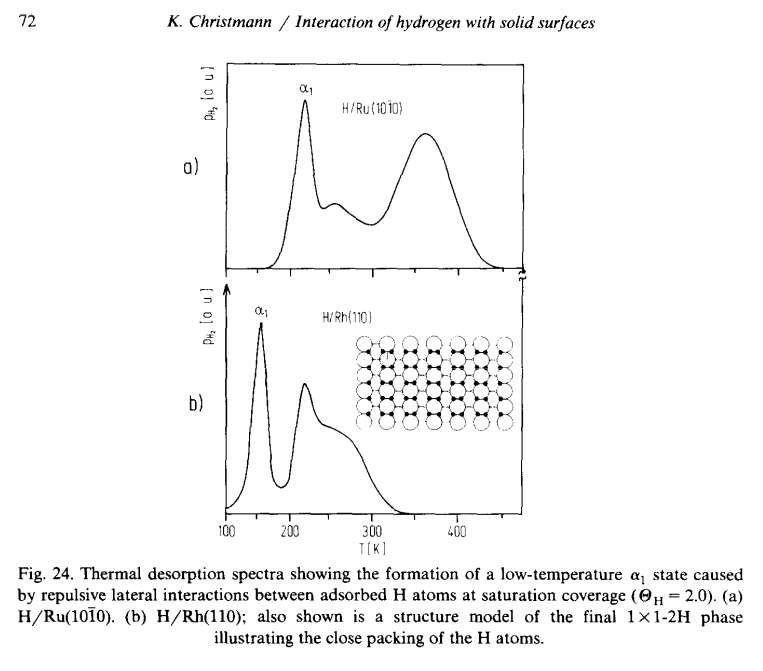
\includegraphics{Christmann_fig24.png}
\caption{Christmann\_fig24.png}
\end{figure}

    Там показан температурный спектр десорбции водорода. Это и есть
дифракционная картина.

По оси икс температура, она пропорциональна импульсу молекул желающих
пройти через дифракционную решётку поверхности и таким образом
десорбироваться. А импульс молекул связан известным соотношением с
длиной волны де Бройля.

Отсюда возникает идея что выходная поверхность должна быть
кристаллографически плотноупакованной поверхностью, чтобы при десорбции
имели место дифракционные эффекты.

    \section{Технологические варианты изготовления никель водородного
кольцара}\label{ux442ux435ux445ux43dux43eux43bux43eux433ux438ux447ux435ux441ux43aux438ux435-ux432ux430ux440ux438ux430ux43dux442ux44b-ux438ux437ux433ux43eux442ux43eux432ux43bux435ux43dux438ux44f-ux43dux438ux43aux435ux43bux44c-ux432ux43eux434ux43eux440ux43eux434ux43dux43eux433ux43e-ux43aux43eux43bux44cux446ux430ux440ux430}

Монокристаллический никель, конечно, известен - но в виде буль, подобных
монокристаллам полупроводников
(http://luch-istok.ru/produktsiya/monokristally-tugoplavkih-metallov/).

\begin{enumerate}
\def\labelenumi{\arabic{enumi})}
\item
  разрезаем булю на пластинки вдоль требуемых hkl, например из одной
  були делаем сотню пластинок Ni (111) а из другой були делаем сотню
  пластинок Ni(110) далее это шлифуется на шлифовальном станке, при этом
  нужно чтобы подобрать условия шлифовки такими, чтобы слоя окислов не
  образовывалось далее слепляем пластинки, хорошо шлифованные пластинки
  прилепятся друг к другу силами Ван дер Ваальса или Казимира. А дальше
  или так тестируем или пытаемся эти пластинки сплавить друг с другом
  повышением температуры
\item
  на пластину требуемой hkl методом напыления вакуумного ионов того же
  никеля но под углом к поверхности пытаемся нанести слой уже с другим
  hkl
\end{enumerate}

    \begin{tcolorbox}[breakable, size=fbox, boxrule=1pt, pad at break*=1mm,colback=cellbackground, colframe=cellborder]
\prompt{In}{incolor}{ }{\boxspacing}
\begin{Verbatim}[commandchars=\\\{\}]

\end{Verbatim}
\end{tcolorbox}

    \section{Химически неравновесные стационарные
состояния}\label{ux445ux438ux43cux438ux447ux435ux441ux43aux438-ux43dux435ux440ux430ux432ux43dux43eux432ux435ux441ux43dux44bux435-ux441ux442ux430ux446ux438ux43eux43dux430ux440ux43dux44bux435-ux441ux43eux441ux442ux43eux44fux43dux438ux44f}

рассмотрим книгу Вызовы к второму началу термодинамики Владислава Чапека

https://isidore.co/CalibreLibrary/Capek,\%20Vladislav/Challenges\%20to\%20the\%20Second\%20Law\%20of\%20Thermodynamics\_\%20Theory\%20and\%20Experiment\%20(4027)/

    в книге у Чапека раздел

7 Chemical Nonequilibrium Steady States

Химически неравновесные стационарные состояния

в котором рассмотрен вариант атомно-молекулярного стационарного
неравновесия как на поверхности металла, так и в газовой фазе.

Чапек рассматривает состояние равновесия реакции

\(H + H = H_2\), как в газовой фазе так и в поверхностном слое металла

При этом он записал две константы равновесия для этой реакции - одна для
поверхностной фазы

\[K(s) = \frac{n(s, A_2)}{n^2(s, A)}\],

другая для газовой фазы

\[K(g) = \frac{n(g, A_2)}{n^2(g, A)}\] (формула 7.1)

Приравняв формулы для скоростей десорбции и адсорбции отдельно для
атомарного и отдельно для молекулярного водорода (это формулы 7.2 и 7.3
соответственно)

\[R_{des} (A) = n(s, A) \nu_{att}(A) P_{des}(A)=\frac{1}{4} n(g, A) v_{A} P_{ads}(A) = R_{ads}(A)\]

\[R_{des} (A_2) = n(s, A_2) \nu_{att}(A_2) P_{des}(A_2)=\frac{1}{4} n(g, A_2) v_{A_2} P_{ads}(A_2) = R_{ads}(A_2)\]

Он применяет микроскопический принцип обратимости, приравнивая
вероятности адсорбции и десорбции (формула 7.4)

\[P_{des}(A) = P_{ads}(A)\]

\[P_{des}(A_2) = P_{ads}(A_2)\]

Получает взаимосвязь между константами диссоциации в газовой фазе и
поверхностной фазе (формула 7.6)

\[K(g) = \frac{v_{A_2}}{2 \nu_0} K(s)\]

Далее он пишет, что поскольку частота \(\nu_0\) вибрации решётки зависит
от материала поверхности, то значит константа диссоциации водорода в
газовой фазе внутри металлической полости полностью определяется типом
поверхности полости

Далее он рассматривая две полости из разного металла замечает, что
степень диссоциации водорода для полостей из разного металла будет
различный

И следовательно возникает разница давлений идеального газа смеси
атомарного и молекулярного водорода потому что суммарная концентрация
двухатомных и одноатомных частиц различна

    Далее он пишет, что если соединить две полости из разного металла
маленьким отвестием то через это отверстие установится стационарный
встречный поток атомарного и молекулярного водорода

    \begin{figure}
\centering
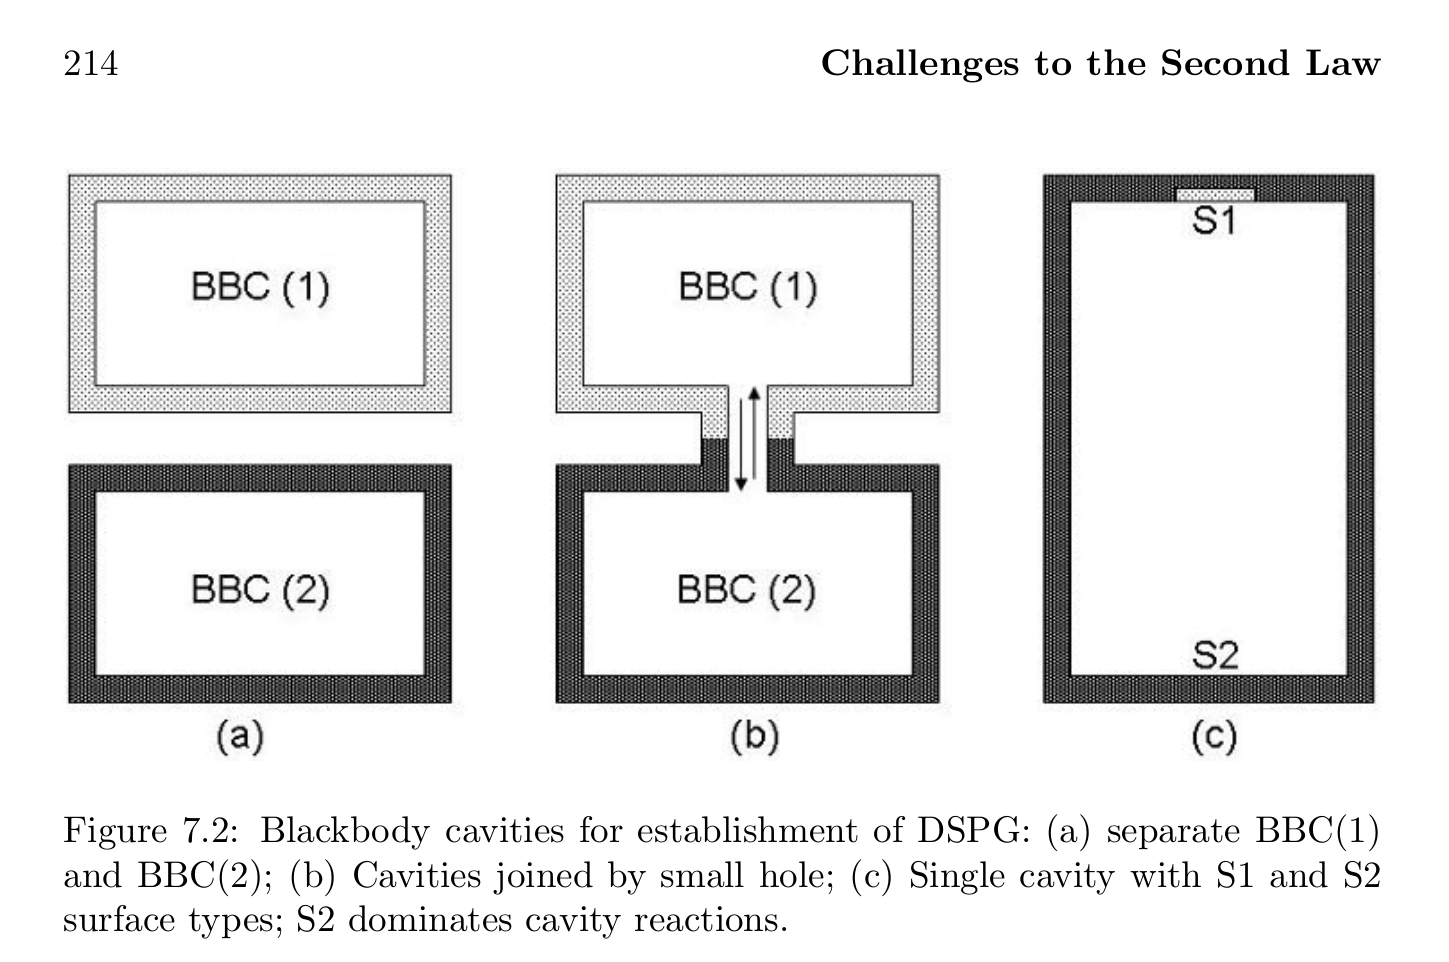
\includegraphics{Capek_fig7.2.png}
\caption{Capek\_fig7.2.png}
\end{figure}

    Таким образом устанавливается стационарное неравновесное состояние.

Условием наступления этого состояния является низкое давление газовой
фазы, в результате чего химическое равновесие в газовой фазе виртуально
отсуствует а зависит от равновесия в поверхностной фазе.

Чапек ссылается на эксперимент с вольфрамом и молибденом.

    \begin{figure}
\centering
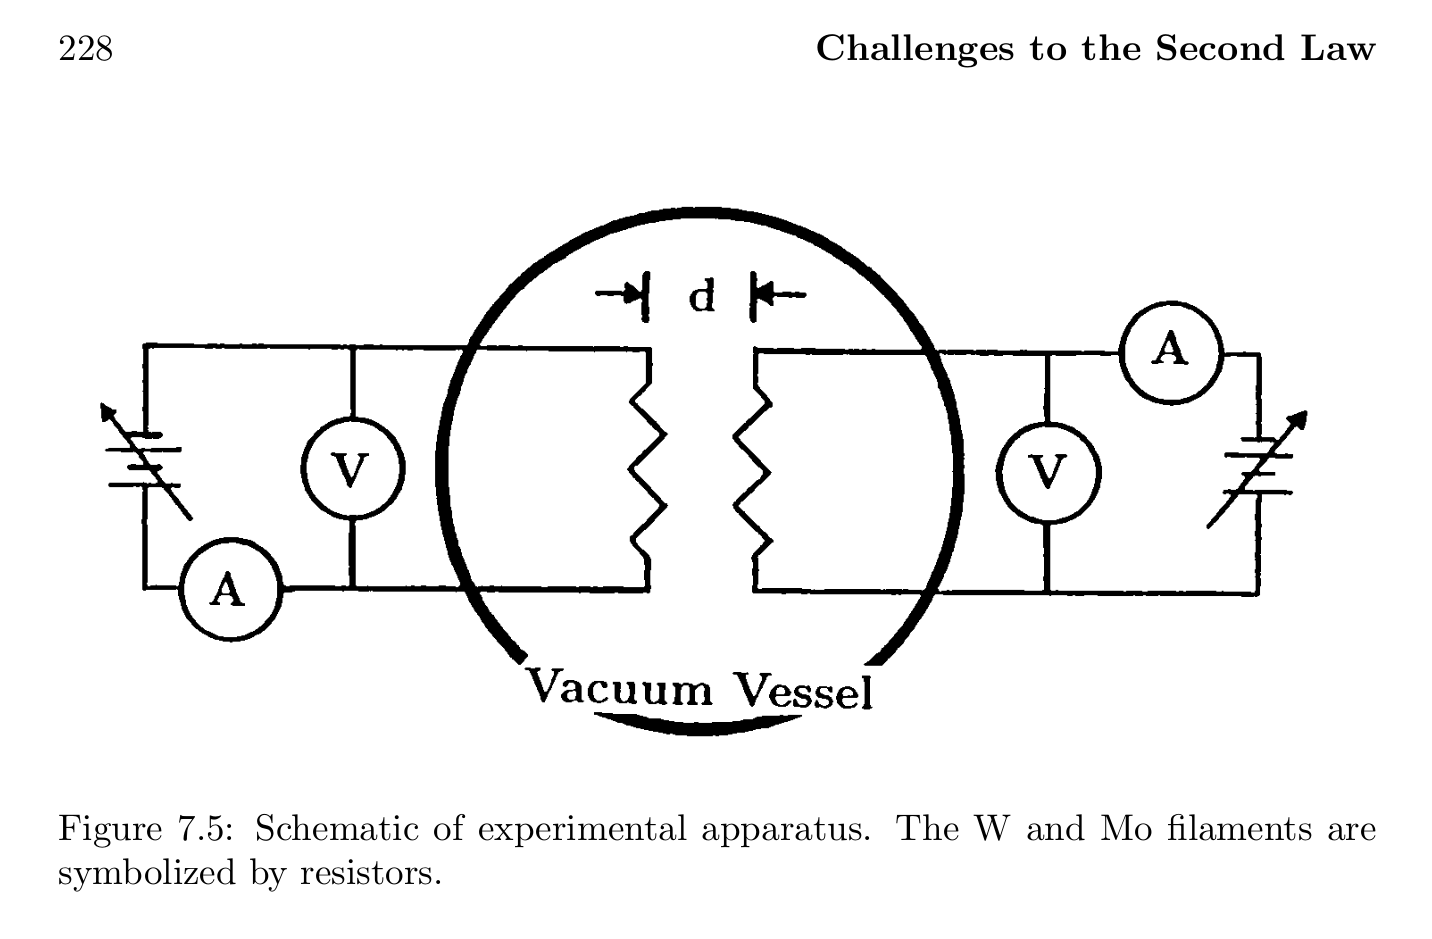
\includegraphics{Capek_fig7.5.png}
\caption{Capek\_fig7.5.png}
\end{figure}

    Это эксперимент в котором наблюдалось для пары металлов вольфрам -
молибден при температуре 2200 кельвин и давлении водорода в газовой фазе
2.5 Торр устанавливается стационарная разность давлений 1 Па.

Это составляет 0.002 часть от общего давления

    \begin{figure}
\centering
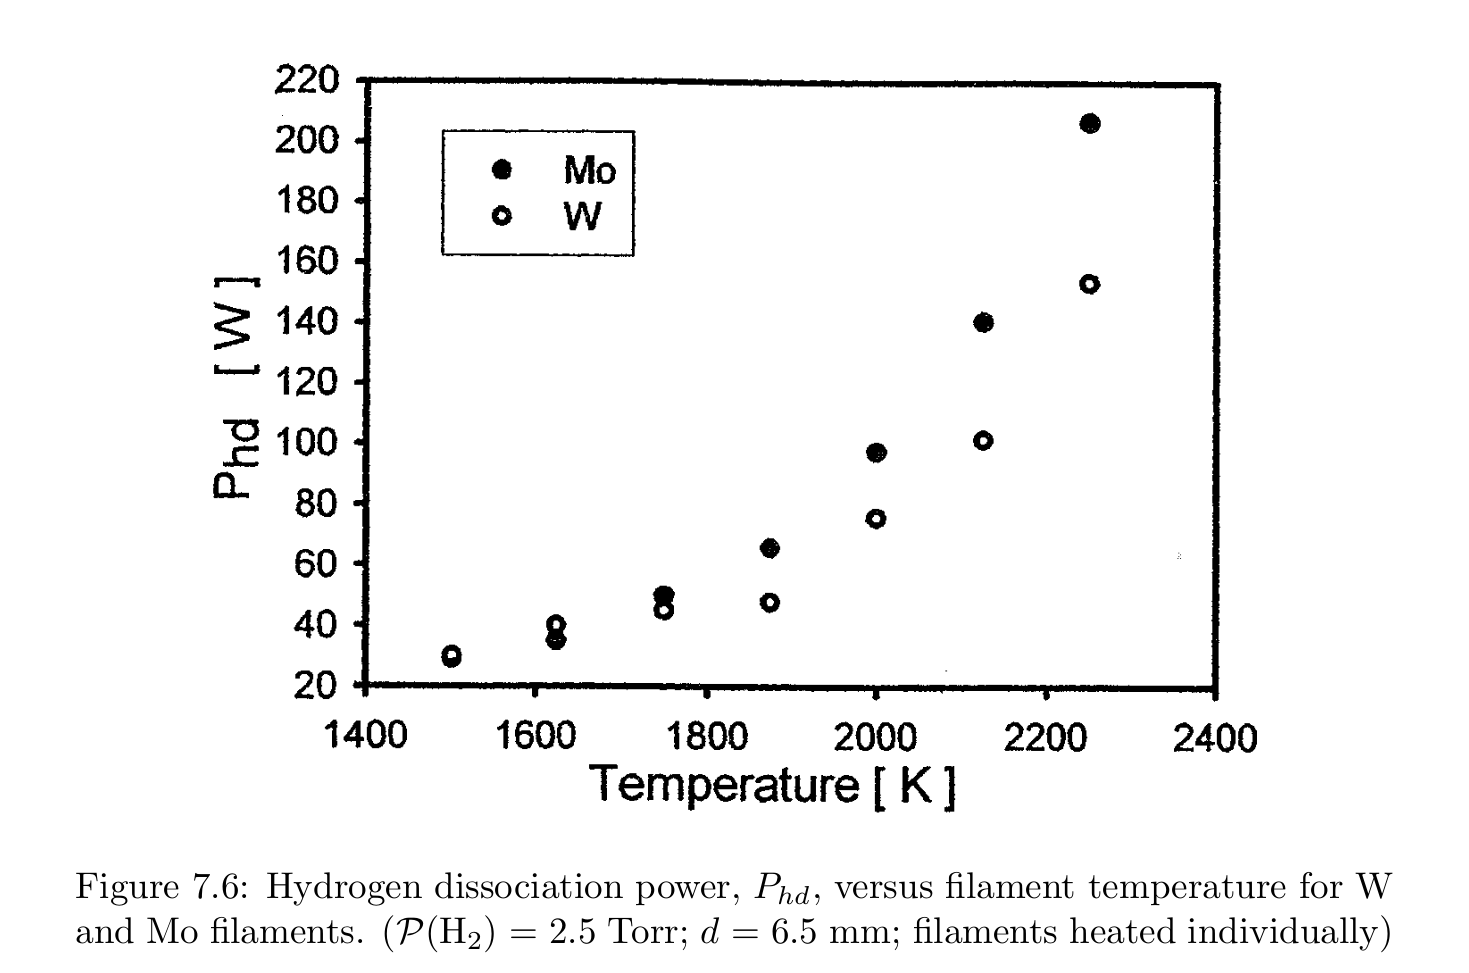
\includegraphics{Capek_fig7.6.png}
\caption{Capek\_fig7.6.png}
\end{figure}

    При увеличении общего давления водорода в газовой фазе стационарная
разность давлений сходит на ноль

    \begin{figure}
\centering
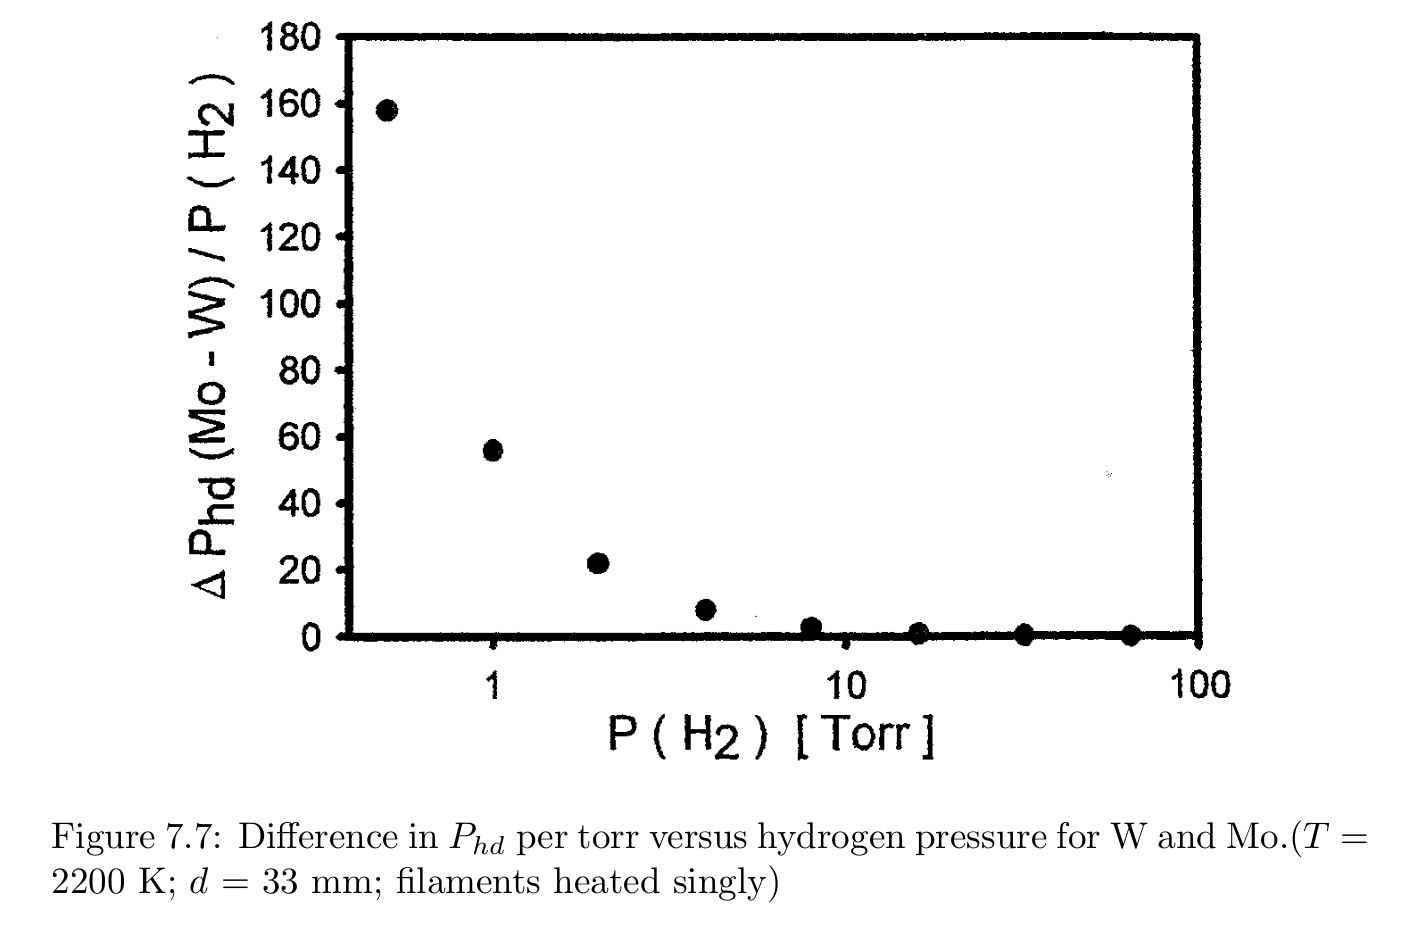
\includegraphics{Capek_fig7.7.png}
\caption{Capek\_fig7.7.png}
\end{figure}

    \begin{tcolorbox}[breakable, size=fbox, boxrule=1pt, pad at break*=1mm,colback=cellbackground, colframe=cellborder]
\prompt{In}{incolor}{ }{\boxspacing}
\begin{Verbatim}[commandchars=\\\{\}]

\end{Verbatim}
\end{tcolorbox}

    \begin{figure}
\centering
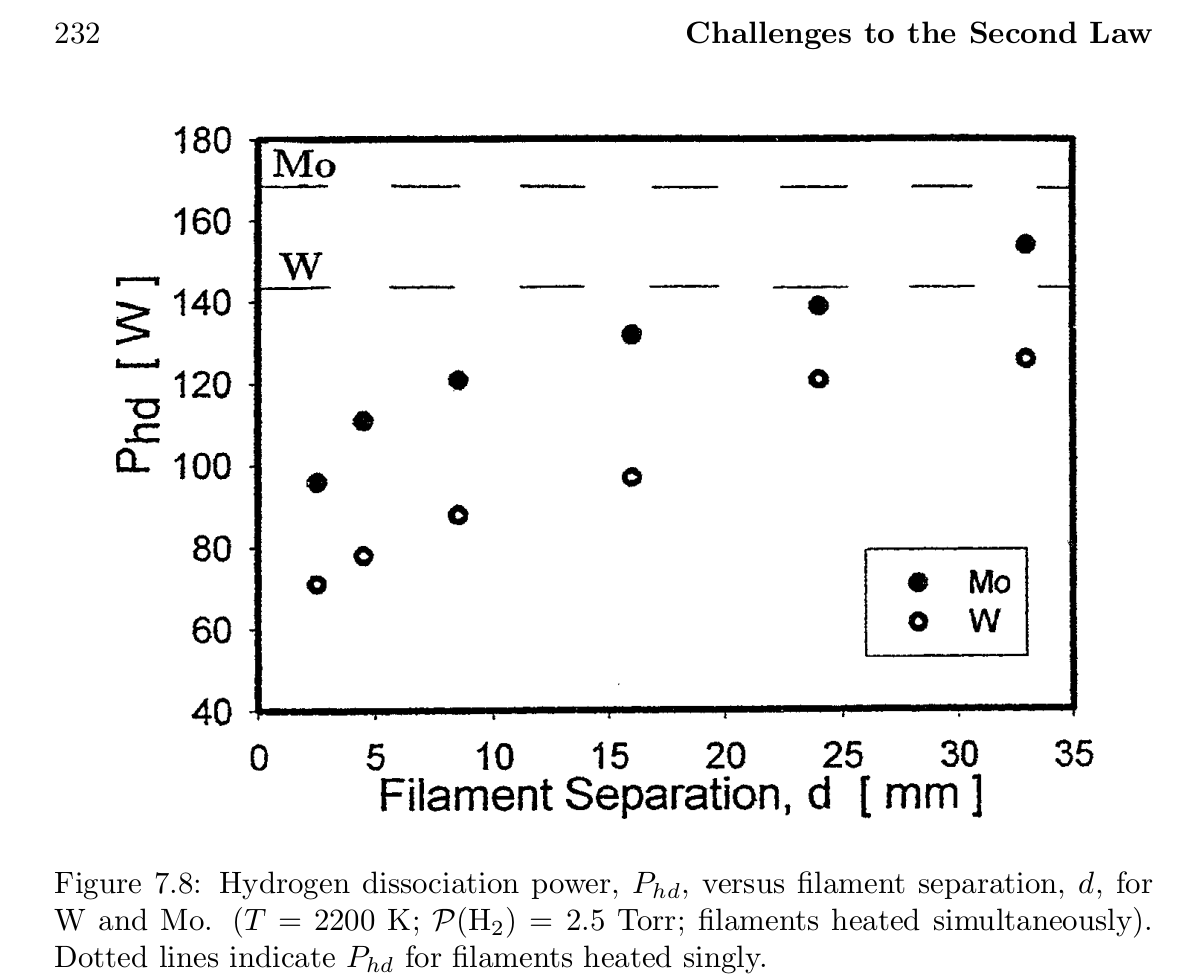
\includegraphics{Capek_fig7.8.png}
\caption{Capek\_fig7.8.png}
\end{figure}

    Однако у Чапека не стояла задача создания сверхпроницаемой мембраны. Он
ставил задачу создания маленькой такой биметаллической вертушечки по
типу модифицированного радиометра Лебедева ради того чтобы в принципе
показать работоспособность ВД2.

    \begin{figure}
\centering
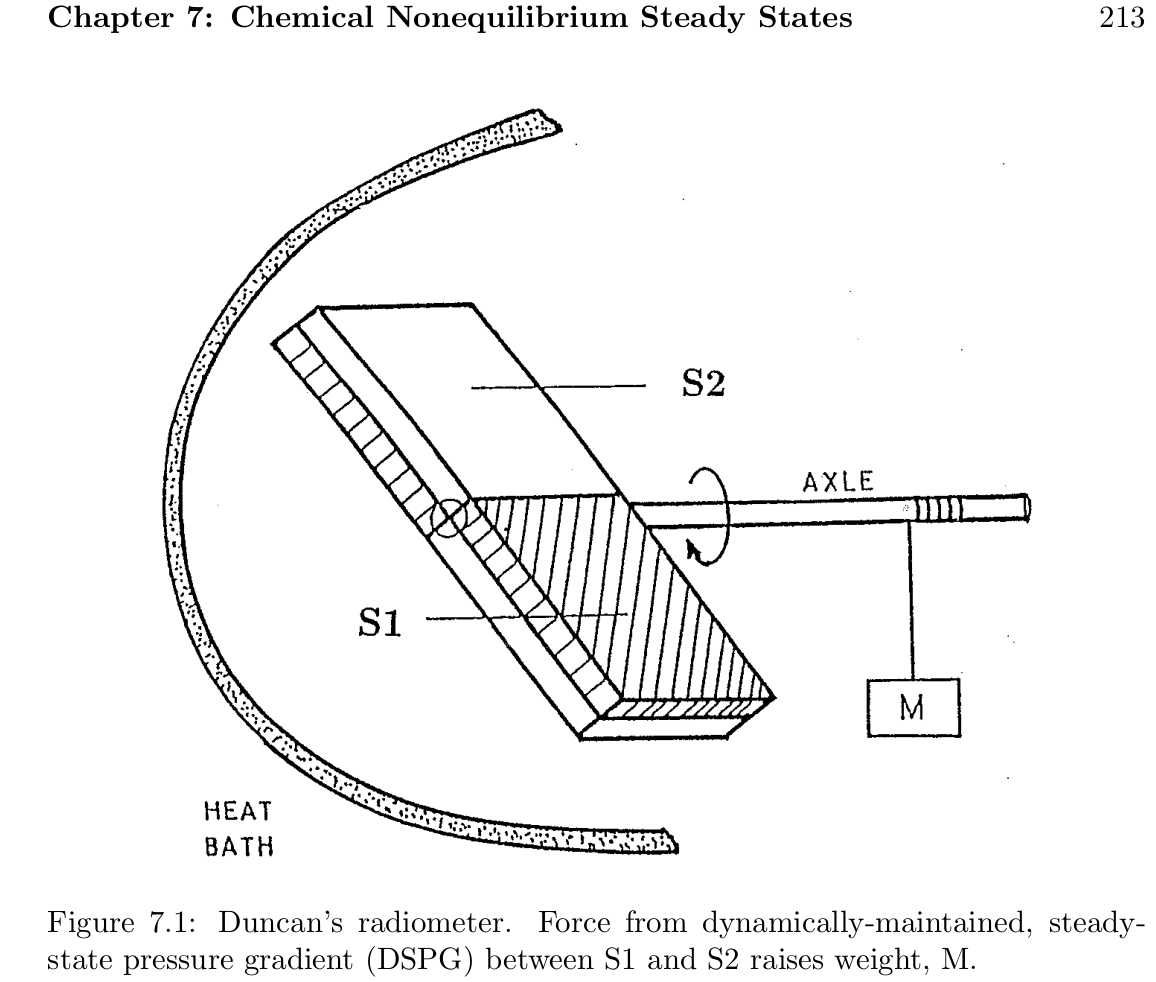
\includegraphics{Capek_fig7.1.png}
\caption{Capek\_fig7.1.png}
\end{figure}

    Проблема именно в том удастся ли подобрать такие условия при которых
мощность ВД2 на основе сверхпрониуаемой мембраны была бы интересно
практически.

Мы я как я уже писал не можем работать подобно Чапеку на эффекте
связанном с выходом атомарного водорода в газовую фазу ибо при
температурах окружающей среды эффект выхода атомарного водорода в
газовую фазу пренебрежимо мал.

Чапек правда пишет о двух двухатомной молекуле He\_2, но по его расчётам
работать с равновесием He + He = He\_2 можно только при температурах
единицы Кельвин.

Мы можем работать только лишь на эффектах о которых я писал и которые
связаны с отклонениями от детального равновесия в процессах десорбции и
сорбции молекулярного водорода.

    \begin{tcolorbox}[breakable, size=fbox, boxrule=1pt, pad at break*=1mm,colback=cellbackground, colframe=cellborder]
\prompt{In}{incolor}{ }{\boxspacing}
\begin{Verbatim}[commandchars=\\\{\}]

\end{Verbatim}
\end{tcolorbox}


    % Add a bibliography block to the postdoc
    
    
    
\end{document}
